% Start preamble
\documentclass[12pt,a4paper]{article}
\usepackage{geometry}
 \geometry{
 a4paper,
 total={170mm,257mm},
 left=20mm,
 top=20mm,
 }
\usepackage[utf8]{inputenc}
\usepackage[T1]{fontenc}
\usepackage[pdftex]{graphicx}
\graphicspath{{./}}
\usepackage{enumitem}
\usepackage{pdfpages}
\usepackage{hyperref}
\usepackage{tikz}
\usepackage{attachfile}
\usepackage{epstopdf}
\usepackage{array}
%\usepackage[table]{xcolor,colorbl}
\setlength{\textwidth}{16cm}
\setlength{\oddsidemargin}{-0.5cm}
\setlength{\evensidemargin}{-0.5cm}
%\setlenght{\headsep}{0cm}
\setlength\parindent{0pt}
%\setlength{\extrarowheight}{3pt}
\usepackage{listings}
%\usepackage{xcolor}

 %%%%%%%%%%%%%%%%%%%%%%%%%%%%%%%%%%%%%%%%%%%%%%%%%%%%%%%%%%%%%%%%%%%%%%%%%%%%%%%% 
%%% ~ Arduino Language - Arduino IDE Colors ~                                  %%%
%%%                                                                            %%%
%%% Kyle Rocha-Brownell | 10/2/2017 | No Licence                               %%%
%%% -------------------------------------------------------------------------- %%%
%%%                                                                            %%%
%%% Place this file in your working directory (next to the latex file you're   %%%
%%% working on).  To add it to your project, place:                            %%%
%%%     %%%%%%%%%%%%%%%%%%%%%%%%%%%%%%%%%%%%%%%%%%%%%%%%%%%%%%%%%%%%%%%%%%%%%%%%%%%%%%%% 
%%% ~ Arduino Language - Arduino IDE Colors ~                                  %%%
%%%                                                                            %%%
%%% Kyle Rocha-Brownell | 10/2/2017 | No Licence                               %%%
%%% -------------------------------------------------------------------------- %%%
%%%                                                                            %%%
%%% Place this file in your working directory (next to the latex file you're   %%%
%%% working on).  To add it to your project, place:                            %%%
%%%     %%%%%%%%%%%%%%%%%%%%%%%%%%%%%%%%%%%%%%%%%%%%%%%%%%%%%%%%%%%%%%%%%%%%%%%%%%%%%%%% 
%%% ~ Arduino Language - Arduino IDE Colors ~                                  %%%
%%%                                                                            %%%
%%% Kyle Rocha-Brownell | 10/2/2017 | No Licence                               %%%
%%% -------------------------------------------------------------------------- %%%
%%%                                                                            %%%
%%% Place this file in your working directory (next to the latex file you're   %%%
%%% working on).  To add it to your project, place:                            %%%
%%%    \input{arduinoLanguage.tex}                                             %%%
%%% somewhere before \begin{document} in your latex file.                      %%%
%%%                                                                            %%%
%%% In your document, place your arduino code between:                         %%%
%%%   \begin{lstlisting}[language=Arduino]                                     %%%
%%% and:                                                                       %%%
%%%   \end{lstlisting}                                                         %%%
%%%                                                                            %%%
%%% Or create your own style to add non-built-in functions and variables.      %%%
%%%                                                                            %%%
 %%%%%%%%%%%%%%%%%%%%%%%%%%%%%%%%%%%%%%%%%%%%%%%%%%%%%%%%%%%%%%%%%%%%%%%%%%%%%%%% 

\usepackage{color}
\usepackage{listings}    
\usepackage{courier}

%%% Define Custom IDE Colors %%%
\definecolor{arduinoGreen}    {rgb} {0.17, 0.43, 0.01}
\definecolor{arduinoGrey}     {rgb} {0.47, 0.47, 0.33}
\definecolor{arduinoOrange}   {rgb} {0.8 , 0.4 , 0   }
\definecolor{arduinoBlue}     {rgb} {0.01, 0.61, 0.98}
\definecolor{arduinoDarkBlue} {rgb} {0.0 , 0.2 , 0.5 }

%%% Define Arduino Language %%%
\lstdefinelanguage{Arduino}{
  language=C++, % begin with default C++ settings 
%
%
  %%% Keyword Color Group 1 %%%  (called KEYWORD3 by arduino)
  keywordstyle=\color{arduinoGreen},   
  deletekeywords={  % remove all arduino keywords that might be in c++
                break, case, override, final, continue, default, do, else, for, 
                if, return, goto, switch, throw, try, while, setup, loop, export, 
                not, or, and, xor, include, define, elif, else, error, if, ifdef, 
                ifndef, pragma, warning,
                HIGH, LOW, INPUT, INPUT_PULLUP, OUTPUT, DEC, BIN, HEX, OCT, PI, 
                HALF_PI, TWO_PI, LSBFIRST, MSBFIRST, CHANGE, FALLING, RISING, 
                DEFAULT, EXTERNAL, INTERNAL, INTERNAL1V1, INTERNAL2V56, LED_BUILTIN, 
                LED_BUILTIN_RX, LED_BUILTIN_TX, DIGITAL_MESSAGE, FIRMATA_STRING, 
                ANALOG_MESSAGE, REPORT_DIGITAL, REPORT_ANALOG, SET_PIN_MODE, 
                SYSTEM_RESET, SYSEX_START, auto, int8_t, int16_t, int32_t, int64_t, 
                uint8_t, uint16_t, uint32_t, uint64_t, char16_t, char32_t, operator, 
                enum, delete, bool, boolean, byte, char, const, false, float, double, 
                null, NULL, int, long, new, private, protected, public, short, 
                signed, static, volatile, String, void, true, unsigned, word, array, 
                sizeof, dynamic_cast, typedef, const_cast, struct, static_cast, union, 
                friend, extern, class, reinterpret_cast, register, explicit, inline, 
                _Bool, complex, _Complex, _Imaginary, atomic_bool, atomic_char, 
                atomic_schar, atomic_uchar, atomic_short, atomic_ushort, atomic_int, 
                atomic_uint, atomic_long, atomic_ulong, atomic_llong, atomic_ullong, 
                virtual, PROGMEM,
                Serial, Serial1, Serial2, Serial3, SerialUSB, Keyboard, Mouse,
                abs, acos, asin, atan, atan2, ceil, constrain, cos, degrees, exp, 
                floor, log, map, max, min, radians, random, randomSeed, round, sin, 
                sq, sqrt, tan, pow, bitRead, bitWrite, bitSet, bitClear, bit, 
                highByte, lowByte, analogReference, analogRead, 
                analogReadResolution, analogWrite, analogWriteResolution, 
                attachInterrupt, detachInterrupt, digitalPinToInterrupt, delay, 
                delayMicroseconds, digitalWrite, digitalRead, interrupts, millis, 
                micros, noInterrupts, noTone, pinMode, pulseIn, pulseInLong, shiftIn, 
                shiftOut, tone, yield, Stream, begin, end, peek, read, print, 
                println, available, availableForWrite, flush, setTimeout, find, 
                findUntil, parseInt, parseFloat, readBytes, readBytesUntil, readString, 
                readStringUntil, trim, toUpperCase, toLowerCase, charAt, compareTo, 
                concat, endsWith, startsWith, equals, equalsIgnoreCase, getBytes, 
                indexOf, lastIndexOf, length, replace, setCharAt, substring, 
                toCharArray, toInt, press, release, releaseAll, accept, click, move, 
                isPressed, isAlphaNumeric, isAlpha, isAscii, isWhitespace, isControl, 
                isDigit, isGraph, isLowerCase, isPrintable, isPunct, isSpace, 
                isUpperCase, isHexadecimalDigit, 
                }, 
  morekeywords={   % add arduino structures to group 1
                break, case, override, final, continue, default, do, else, for, 
                if, return, goto, switch, throw, try, while, setup, loop, export, 
                not, or, and, xor, include, define, elif, else, error, if, ifdef, 
                ifndef, pragma, warning,
                }, 
% 
%
  %%% Keyword Color Group 2 %%%  (called LITERAL1 by arduino)
  keywordstyle=[2]\color{arduinoBlue},   
  keywords=[2]{   % add variables and dataTypes as 2nd group  
                HIGH, LOW, INPUT, INPUT_PULLUP, OUTPUT, DEC, BIN, HEX, OCT, PI, 
                HALF_PI, TWO_PI, LSBFIRST, MSBFIRST, CHANGE, FALLING, RISING, 
                DEFAULT, EXTERNAL, INTERNAL, INTERNAL1V1, INTERNAL2V56, LED_BUILTIN, 
                LED_BUILTIN_RX, LED_BUILTIN_TX, DIGITAL_MESSAGE, FIRMATA_STRING, 
                ANALOG_MESSAGE, REPORT_DIGITAL, REPORT_ANALOG, SET_PIN_MODE, 
                SYSTEM_RESET, SYSEX_START, auto, int8_t, int16_t, int32_t, int64_t, 
                uint8_t, uint16_t, uint32_t, uint64_t, char16_t, char32_t, operator, 
                enum, delete, bool, boolean, byte, char, const, false, float, double, 
                null, NULL, int, long, new, private, protected, public, short, 
                signed, static, volatile, String, void, true, unsigned, word, array, 
                sizeof, dynamic_cast, typedef, const_cast, struct, static_cast, union, 
                friend, extern, class, reinterpret_cast, register, explicit, inline, 
                _Bool, complex, _Complex, _Imaginary, atomic_bool, atomic_char, 
                atomic_schar, atomic_uchar, atomic_short, atomic_ushort, atomic_int, 
                atomic_uint, atomic_long, atomic_ulong, atomic_llong, atomic_ullong, 
                virtual, PROGMEM,
                },  
% 
%
  %%% Keyword Color Group 3 %%%  (called KEYWORD1 by arduino)
  keywordstyle=[3]\bfseries\color{arduinoOrange},
  keywords=[3]{  % add built-in functions as a 3rd group
                Serial, Serial1, Serial2, Serial3, SerialUSB, Keyboard, Mouse,
                },      
%
%
  %%% Keyword Color Group 4 %%%  (called KEYWORD2 by arduino)
  keywordstyle=[4]\color{arduinoOrange},
  keywords=[4]{  % add more built-in functions as a 4th group
                abs, acos, asin, atan, atan2, ceil, constrain, cos, degrees, exp, 
                floor, log, map, max, min, radians, random, randomSeed, round, sin, 
                sq, sqrt, tan, pow, bitRead, bitWrite, bitSet, bitClear, bit, 
                highByte, lowByte, analogReference, analogRead, 
                analogReadResolution, analogWrite, analogWriteResolution, 
                attachInterrupt, detachInterrupt, digitalPinToInterrupt, delay, 
                delayMicroseconds, digitalWrite, digitalRead, interrupts, millis, 
                micros, noInterrupts, noTone, pinMode, pulseIn, pulseInLong, shiftIn, 
                shiftOut, tone, yield, Stream, begin, end, peek, read, print, 
                println, available, availableForWrite, flush, setTimeout, find, 
                findUntil, parseInt, parseFloat, readBytes, readBytesUntil, readString, 
                readStringUntil, trim, toUpperCase, toLowerCase, charAt, compareTo, 
                concat, endsWith, startsWith, equals, equalsIgnoreCase, getBytes, 
                indexOf, lastIndexOf, length, replace, setCharAt, substring, 
                toCharArray, toInt, press, release, releaseAll, accept, click, move, 
                isPressed, isAlphaNumeric, isAlpha, isAscii, isWhitespace, isControl, 
                isDigit, isGraph, isLowerCase, isPrintable, isPunct, isSpace, 
                isUpperCase, isHexadecimalDigit, 
                },      
%
%
  %%% Set Other Colors %%%
  stringstyle=\color{arduinoDarkBlue},    
  commentstyle=\color{arduinoGrey},    
%          
%   
  %%%% Line Numbering %%%%
%  numbers=left,                    
%  numbersep=5pt,                   
%  numberstyle=\color{arduinoGrey},    
  %stepnumber=2,                      % show every 2 line numbers
%
%
  %%%% Code Box Style %%%%
  breaklines=true,                    % wordwrapping
  tabsize=8,         
  basicstyle=\ttfamily  
}
                                             %%%
%%% somewhere before \begin{document} in your latex file.                      %%%
%%%                                                                            %%%
%%% In your document, place your arduino code between:                         %%%
%%%   \begin{lstlisting}[language=Arduino]                                     %%%
%%% and:                                                                       %%%
%%%   \end{lstlisting}                                                         %%%
%%%                                                                            %%%
%%% Or create your own style to add non-built-in functions and variables.      %%%
%%%                                                                            %%%
 %%%%%%%%%%%%%%%%%%%%%%%%%%%%%%%%%%%%%%%%%%%%%%%%%%%%%%%%%%%%%%%%%%%%%%%%%%%%%%%% 

\usepackage{color}
\usepackage{listings}    
\usepackage{courier}

%%% Define Custom IDE Colors %%%
\definecolor{arduinoGreen}    {rgb} {0.17, 0.43, 0.01}
\definecolor{arduinoGrey}     {rgb} {0.47, 0.47, 0.33}
\definecolor{arduinoOrange}   {rgb} {0.8 , 0.4 , 0   }
\definecolor{arduinoBlue}     {rgb} {0.01, 0.61, 0.98}
\definecolor{arduinoDarkBlue} {rgb} {0.0 , 0.2 , 0.5 }

%%% Define Arduino Language %%%
\lstdefinelanguage{Arduino}{
  language=C++, % begin with default C++ settings 
%
%
  %%% Keyword Color Group 1 %%%  (called KEYWORD3 by arduino)
  keywordstyle=\color{arduinoGreen},   
  deletekeywords={  % remove all arduino keywords that might be in c++
                break, case, override, final, continue, default, do, else, for, 
                if, return, goto, switch, throw, try, while, setup, loop, export, 
                not, or, and, xor, include, define, elif, else, error, if, ifdef, 
                ifndef, pragma, warning,
                HIGH, LOW, INPUT, INPUT_PULLUP, OUTPUT, DEC, BIN, HEX, OCT, PI, 
                HALF_PI, TWO_PI, LSBFIRST, MSBFIRST, CHANGE, FALLING, RISING, 
                DEFAULT, EXTERNAL, INTERNAL, INTERNAL1V1, INTERNAL2V56, LED_BUILTIN, 
                LED_BUILTIN_RX, LED_BUILTIN_TX, DIGITAL_MESSAGE, FIRMATA_STRING, 
                ANALOG_MESSAGE, REPORT_DIGITAL, REPORT_ANALOG, SET_PIN_MODE, 
                SYSTEM_RESET, SYSEX_START, auto, int8_t, int16_t, int32_t, int64_t, 
                uint8_t, uint16_t, uint32_t, uint64_t, char16_t, char32_t, operator, 
                enum, delete, bool, boolean, byte, char, const, false, float, double, 
                null, NULL, int, long, new, private, protected, public, short, 
                signed, static, volatile, String, void, true, unsigned, word, array, 
                sizeof, dynamic_cast, typedef, const_cast, struct, static_cast, union, 
                friend, extern, class, reinterpret_cast, register, explicit, inline, 
                _Bool, complex, _Complex, _Imaginary, atomic_bool, atomic_char, 
                atomic_schar, atomic_uchar, atomic_short, atomic_ushort, atomic_int, 
                atomic_uint, atomic_long, atomic_ulong, atomic_llong, atomic_ullong, 
                virtual, PROGMEM,
                Serial, Serial1, Serial2, Serial3, SerialUSB, Keyboard, Mouse,
                abs, acos, asin, atan, atan2, ceil, constrain, cos, degrees, exp, 
                floor, log, map, max, min, radians, random, randomSeed, round, sin, 
                sq, sqrt, tan, pow, bitRead, bitWrite, bitSet, bitClear, bit, 
                highByte, lowByte, analogReference, analogRead, 
                analogReadResolution, analogWrite, analogWriteResolution, 
                attachInterrupt, detachInterrupt, digitalPinToInterrupt, delay, 
                delayMicroseconds, digitalWrite, digitalRead, interrupts, millis, 
                micros, noInterrupts, noTone, pinMode, pulseIn, pulseInLong, shiftIn, 
                shiftOut, tone, yield, Stream, begin, end, peek, read, print, 
                println, available, availableForWrite, flush, setTimeout, find, 
                findUntil, parseInt, parseFloat, readBytes, readBytesUntil, readString, 
                readStringUntil, trim, toUpperCase, toLowerCase, charAt, compareTo, 
                concat, endsWith, startsWith, equals, equalsIgnoreCase, getBytes, 
                indexOf, lastIndexOf, length, replace, setCharAt, substring, 
                toCharArray, toInt, press, release, releaseAll, accept, click, move, 
                isPressed, isAlphaNumeric, isAlpha, isAscii, isWhitespace, isControl, 
                isDigit, isGraph, isLowerCase, isPrintable, isPunct, isSpace, 
                isUpperCase, isHexadecimalDigit, 
                }, 
  morekeywords={   % add arduino structures to group 1
                break, case, override, final, continue, default, do, else, for, 
                if, return, goto, switch, throw, try, while, setup, loop, export, 
                not, or, and, xor, include, define, elif, else, error, if, ifdef, 
                ifndef, pragma, warning,
                }, 
% 
%
  %%% Keyword Color Group 2 %%%  (called LITERAL1 by arduino)
  keywordstyle=[2]\color{arduinoBlue},   
  keywords=[2]{   % add variables and dataTypes as 2nd group  
                HIGH, LOW, INPUT, INPUT_PULLUP, OUTPUT, DEC, BIN, HEX, OCT, PI, 
                HALF_PI, TWO_PI, LSBFIRST, MSBFIRST, CHANGE, FALLING, RISING, 
                DEFAULT, EXTERNAL, INTERNAL, INTERNAL1V1, INTERNAL2V56, LED_BUILTIN, 
                LED_BUILTIN_RX, LED_BUILTIN_TX, DIGITAL_MESSAGE, FIRMATA_STRING, 
                ANALOG_MESSAGE, REPORT_DIGITAL, REPORT_ANALOG, SET_PIN_MODE, 
                SYSTEM_RESET, SYSEX_START, auto, int8_t, int16_t, int32_t, int64_t, 
                uint8_t, uint16_t, uint32_t, uint64_t, char16_t, char32_t, operator, 
                enum, delete, bool, boolean, byte, char, const, false, float, double, 
                null, NULL, int, long, new, private, protected, public, short, 
                signed, static, volatile, String, void, true, unsigned, word, array, 
                sizeof, dynamic_cast, typedef, const_cast, struct, static_cast, union, 
                friend, extern, class, reinterpret_cast, register, explicit, inline, 
                _Bool, complex, _Complex, _Imaginary, atomic_bool, atomic_char, 
                atomic_schar, atomic_uchar, atomic_short, atomic_ushort, atomic_int, 
                atomic_uint, atomic_long, atomic_ulong, atomic_llong, atomic_ullong, 
                virtual, PROGMEM,
                },  
% 
%
  %%% Keyword Color Group 3 %%%  (called KEYWORD1 by arduino)
  keywordstyle=[3]\bfseries\color{arduinoOrange},
  keywords=[3]{  % add built-in functions as a 3rd group
                Serial, Serial1, Serial2, Serial3, SerialUSB, Keyboard, Mouse,
                },      
%
%
  %%% Keyword Color Group 4 %%%  (called KEYWORD2 by arduino)
  keywordstyle=[4]\color{arduinoOrange},
  keywords=[4]{  % add more built-in functions as a 4th group
                abs, acos, asin, atan, atan2, ceil, constrain, cos, degrees, exp, 
                floor, log, map, max, min, radians, random, randomSeed, round, sin, 
                sq, sqrt, tan, pow, bitRead, bitWrite, bitSet, bitClear, bit, 
                highByte, lowByte, analogReference, analogRead, 
                analogReadResolution, analogWrite, analogWriteResolution, 
                attachInterrupt, detachInterrupt, digitalPinToInterrupt, delay, 
                delayMicroseconds, digitalWrite, digitalRead, interrupts, millis, 
                micros, noInterrupts, noTone, pinMode, pulseIn, pulseInLong, shiftIn, 
                shiftOut, tone, yield, Stream, begin, end, peek, read, print, 
                println, available, availableForWrite, flush, setTimeout, find, 
                findUntil, parseInt, parseFloat, readBytes, readBytesUntil, readString, 
                readStringUntil, trim, toUpperCase, toLowerCase, charAt, compareTo, 
                concat, endsWith, startsWith, equals, equalsIgnoreCase, getBytes, 
                indexOf, lastIndexOf, length, replace, setCharAt, substring, 
                toCharArray, toInt, press, release, releaseAll, accept, click, move, 
                isPressed, isAlphaNumeric, isAlpha, isAscii, isWhitespace, isControl, 
                isDigit, isGraph, isLowerCase, isPrintable, isPunct, isSpace, 
                isUpperCase, isHexadecimalDigit, 
                },      
%
%
  %%% Set Other Colors %%%
  stringstyle=\color{arduinoDarkBlue},    
  commentstyle=\color{arduinoGrey},    
%          
%   
  %%%% Line Numbering %%%%
%  numbers=left,                    
%  numbersep=5pt,                   
%  numberstyle=\color{arduinoGrey},    
  %stepnumber=2,                      % show every 2 line numbers
%
%
  %%%% Code Box Style %%%%
  breaklines=true,                    % wordwrapping
  tabsize=8,         
  basicstyle=\ttfamily  
}
                                             %%%
%%% somewhere before \begin{document} in your latex file.                      %%%
%%%                                                                            %%%
%%% In your document, place your arduino code between:                         %%%
%%%   \begin{lstlisting}[language=Arduino]                                     %%%
%%% and:                                                                       %%%
%%%   \end{lstlisting}                                                         %%%
%%%                                                                            %%%
%%% Or create your own style to add non-built-in functions and variables.      %%%
%%%                                                                            %%%
 %%%%%%%%%%%%%%%%%%%%%%%%%%%%%%%%%%%%%%%%%%%%%%%%%%%%%%%%%%%%%%%%%%%%%%%%%%%%%%%% 

\usepackage{color}
\usepackage{listings}    
\usepackage{courier}

%%% Define Custom IDE Colors %%%
\definecolor{arduinoGreen}    {rgb} {0.17, 0.43, 0.01}
\definecolor{arduinoGrey}     {rgb} {0.47, 0.47, 0.33}
\definecolor{arduinoOrange}   {rgb} {0.8 , 0.4 , 0   }
\definecolor{arduinoBlue}     {rgb} {0.01, 0.61, 0.98}
\definecolor{arduinoDarkBlue} {rgb} {0.0 , 0.2 , 0.5 }

%%% Define Arduino Language %%%
\lstdefinelanguage{Arduino}{
  language=C++, % begin with default C++ settings 
%
%
  %%% Keyword Color Group 1 %%%  (called KEYWORD3 by arduino)
  keywordstyle=\color{arduinoGreen},   
  deletekeywords={  % remove all arduino keywords that might be in c++
                break, case, override, final, continue, default, do, else, for, 
                if, return, goto, switch, throw, try, while, setup, loop, export, 
                not, or, and, xor, include, define, elif, else, error, if, ifdef, 
                ifndef, pragma, warning,
                HIGH, LOW, INPUT, INPUT_PULLUP, OUTPUT, DEC, BIN, HEX, OCT, PI, 
                HALF_PI, TWO_PI, LSBFIRST, MSBFIRST, CHANGE, FALLING, RISING, 
                DEFAULT, EXTERNAL, INTERNAL, INTERNAL1V1, INTERNAL2V56, LED_BUILTIN, 
                LED_BUILTIN_RX, LED_BUILTIN_TX, DIGITAL_MESSAGE, FIRMATA_STRING, 
                ANALOG_MESSAGE, REPORT_DIGITAL, REPORT_ANALOG, SET_PIN_MODE, 
                SYSTEM_RESET, SYSEX_START, auto, int8_t, int16_t, int32_t, int64_t, 
                uint8_t, uint16_t, uint32_t, uint64_t, char16_t, char32_t, operator, 
                enum, delete, bool, boolean, byte, char, const, false, float, double, 
                null, NULL, int, long, new, private, protected, public, short, 
                signed, static, volatile, String, void, true, unsigned, word, array, 
                sizeof, dynamic_cast, typedef, const_cast, struct, static_cast, union, 
                friend, extern, class, reinterpret_cast, register, explicit, inline, 
                _Bool, complex, _Complex, _Imaginary, atomic_bool, atomic_char, 
                atomic_schar, atomic_uchar, atomic_short, atomic_ushort, atomic_int, 
                atomic_uint, atomic_long, atomic_ulong, atomic_llong, atomic_ullong, 
                virtual, PROGMEM,
                Serial, Serial1, Serial2, Serial3, SerialUSB, Keyboard, Mouse,
                abs, acos, asin, atan, atan2, ceil, constrain, cos, degrees, exp, 
                floor, log, map, max, min, radians, random, randomSeed, round, sin, 
                sq, sqrt, tan, pow, bitRead, bitWrite, bitSet, bitClear, bit, 
                highByte, lowByte, analogReference, analogRead, 
                analogReadResolution, analogWrite, analogWriteResolution, 
                attachInterrupt, detachInterrupt, digitalPinToInterrupt, delay, 
                delayMicroseconds, digitalWrite, digitalRead, interrupts, millis, 
                micros, noInterrupts, noTone, pinMode, pulseIn, pulseInLong, shiftIn, 
                shiftOut, tone, yield, Stream, begin, end, peek, read, print, 
                println, available, availableForWrite, flush, setTimeout, find, 
                findUntil, parseInt, parseFloat, readBytes, readBytesUntil, readString, 
                readStringUntil, trim, toUpperCase, toLowerCase, charAt, compareTo, 
                concat, endsWith, startsWith, equals, equalsIgnoreCase, getBytes, 
                indexOf, lastIndexOf, length, replace, setCharAt, substring, 
                toCharArray, toInt, press, release, releaseAll, accept, click, move, 
                isPressed, isAlphaNumeric, isAlpha, isAscii, isWhitespace, isControl, 
                isDigit, isGraph, isLowerCase, isPrintable, isPunct, isSpace, 
                isUpperCase, isHexadecimalDigit, 
                }, 
  morekeywords={   % add arduino structures to group 1
                break, case, override, final, continue, default, do, else, for, 
                if, return, goto, switch, throw, try, while, setup, loop, export, 
                not, or, and, xor, include, define, elif, else, error, if, ifdef, 
                ifndef, pragma, warning,
                }, 
% 
%
  %%% Keyword Color Group 2 %%%  (called LITERAL1 by arduino)
  keywordstyle=[2]\color{arduinoBlue},   
  keywords=[2]{   % add variables and dataTypes as 2nd group  
                HIGH, LOW, INPUT, INPUT_PULLUP, OUTPUT, DEC, BIN, HEX, OCT, PI, 
                HALF_PI, TWO_PI, LSBFIRST, MSBFIRST, CHANGE, FALLING, RISING, 
                DEFAULT, EXTERNAL, INTERNAL, INTERNAL1V1, INTERNAL2V56, LED_BUILTIN, 
                LED_BUILTIN_RX, LED_BUILTIN_TX, DIGITAL_MESSAGE, FIRMATA_STRING, 
                ANALOG_MESSAGE, REPORT_DIGITAL, REPORT_ANALOG, SET_PIN_MODE, 
                SYSTEM_RESET, SYSEX_START, auto, int8_t, int16_t, int32_t, int64_t, 
                uint8_t, uint16_t, uint32_t, uint64_t, char16_t, char32_t, operator, 
                enum, delete, bool, boolean, byte, char, const, false, float, double, 
                null, NULL, int, long, new, private, protected, public, short, 
                signed, static, volatile, String, void, true, unsigned, word, array, 
                sizeof, dynamic_cast, typedef, const_cast, struct, static_cast, union, 
                friend, extern, class, reinterpret_cast, register, explicit, inline, 
                _Bool, complex, _Complex, _Imaginary, atomic_bool, atomic_char, 
                atomic_schar, atomic_uchar, atomic_short, atomic_ushort, atomic_int, 
                atomic_uint, atomic_long, atomic_ulong, atomic_llong, atomic_ullong, 
                virtual, PROGMEM,
                },  
% 
%
  %%% Keyword Color Group 3 %%%  (called KEYWORD1 by arduino)
  keywordstyle=[3]\bfseries\color{arduinoOrange},
  keywords=[3]{  % add built-in functions as a 3rd group
                Serial, Serial1, Serial2, Serial3, SerialUSB, Keyboard, Mouse,
                },      
%
%
  %%% Keyword Color Group 4 %%%  (called KEYWORD2 by arduino)
  keywordstyle=[4]\color{arduinoOrange},
  keywords=[4]{  % add more built-in functions as a 4th group
                abs, acos, asin, atan, atan2, ceil, constrain, cos, degrees, exp, 
                floor, log, map, max, min, radians, random, randomSeed, round, sin, 
                sq, sqrt, tan, pow, bitRead, bitWrite, bitSet, bitClear, bit, 
                highByte, lowByte, analogReference, analogRead, 
                analogReadResolution, analogWrite, analogWriteResolution, 
                attachInterrupt, detachInterrupt, digitalPinToInterrupt, delay, 
                delayMicroseconds, digitalWrite, digitalRead, interrupts, millis, 
                micros, noInterrupts, noTone, pinMode, pulseIn, pulseInLong, shiftIn, 
                shiftOut, tone, yield, Stream, begin, end, peek, read, print, 
                println, available, availableForWrite, flush, setTimeout, find, 
                findUntil, parseInt, parseFloat, readBytes, readBytesUntil, readString, 
                readStringUntil, trim, toUpperCase, toLowerCase, charAt, compareTo, 
                concat, endsWith, startsWith, equals, equalsIgnoreCase, getBytes, 
                indexOf, lastIndexOf, length, replace, setCharAt, substring, 
                toCharArray, toInt, press, release, releaseAll, accept, click, move, 
                isPressed, isAlphaNumeric, isAlpha, isAscii, isWhitespace, isControl, 
                isDigit, isGraph, isLowerCase, isPrintable, isPunct, isSpace, 
                isUpperCase, isHexadecimalDigit, 
                },      
%
%
  %%% Set Other Colors %%%
  stringstyle=\color{arduinoDarkBlue},    
  commentstyle=\color{arduinoGrey},    
%          
%   
  %%%% Line Numbering %%%%
%  numbers=left,                    
%  numbersep=5pt,                   
%  numberstyle=\color{arduinoGrey},    
  %stepnumber=2,                      % show every 2 line numbers
%
%
  %%%% Code Box Style %%%%
  breaklines=true,                    % wordwrapping
  tabsize=8,         
  basicstyle=\ttfamily  
}

%%%%%% Counting oppgaves %%%%%%
 \newcount\questnum \questnum=0
 \def\oppgave{
            \advance\questnum by 1
            \ifnum \questnum > 0
                 \hrule
                 \vskip 3pt
                 \leftline{Oppgave \the\questnum}
                 \vskip 3pt \fi}
 %%%%%%%%%%%%%%%%%%%%%%
%%%%%%%%%%%%%%%%%%%%%%


%%%%%% Counting answers %%%%%%
\newcount\answnum \answnum=0
\def\svar{
           \advance\answnum by 1
           \ifnum \answnum > 0
                \hrule
                \vskip 3pt
                \leftline{Svar \the\answnum}
                \vskip 3pt \fi}
%%%%%%%%%%%%%%%%%%%%%%


%%%%%% Counting notes %%%%%%
\newcount\explnum \explnum=0
\def\notes{
           \advance\explnum by 1
           \ifnum \explnum > 0
                \hrule
                \vskip 3pt
                \leftline{Notes \the\explnum}
                \vskip 3pt \fi}
%%%%%%%%%%%%%%%%%%%%%%

% End preamble

\begin{document}
% !TEX root = /home/fred-olav/afgv/src/preamble.tex
\centerline{\bf Tittel på leksjonen}  \bigskip

Kompetansemål:
\begin{itemize}[noitemsep]

	\item utføre arbeid på automatiserte anlegg fagmessig, nøyaktig og i overensstemmelse med krav til helse, miljø og sikkerhet og rutiner for kvalitetssikring og internkontroll
	\item utføre risikovurdering og vurdere tiltak for ivaretakelse av person- og maskinsikkerhet
	\item vurdere hvilke regelverk og normer som gjelder for arbeidet som skal utføres og anvende dette
	\item planlegge, utføre, vurdere kvalitet, sluttkontrollere og dokumentere arbeidet
	\item planlegge, programmere, montere og idriftsette programmerbare styresystemer
	\item endre og tilpasse skjermbilder for grensesnitt mellom menneske og maskin
	\item anvende ulike elektroniske kommunikasjonssystemer i automatiserte anlegg
	\item vurdere datasikkerhet i automatiserte anlegg
	\item tegne, lese og forklare instrumenterte prosessflytskjemaer og bruke annen relevant dokumentasjon for automatiserte anlegg
	\item montere, konfigurere, kalibrere og idriftsettelse digitale og analoge målesystemer
	\item idriftsette og optimalisere regulatorer basert på prosessbehov
	\item montere og idriftsette ulike typer pådragsorganer med tilhørende forstillingselementer og hjelpeutstyr
	\item programmere, idriftsette samt gjøre rede for roboters funksjon og anvendelse i produksjonsanlegg
	\item måle fysiske størrelser i automatiserte anlegg
	\item feilsøke og rette feil i automatiserte anlegg
	\item bruke gjeldende regelverk og normer for elektriske installasjoner på maskiner
	\item bruke gjeldende regelverk og normer for installasjon av elektroniske kommunikasjonssystemer
	\item beskrive ulike vedlikeholdssystemer og -rutiner knyttet til automatiserte anlegg, og anvende et av disse
	\item redegjøre for bedriftens organisasjonsoppbygging og bedriftens verdiskapning i et samfunnsperspektiv
	\item dokumentere egen opplæring i automatiseringssystemer
\end{itemize}
	Læringsmål
	\begin{itemize}[noitemsep]
		\item Kunne 
		\item Kunne 
	\end{itemize}

	Forkunnskaper

	\begin{itemize}[noitemsep]
		\item 

	\end{itemize}
\textbf{Teori}\\\\
afgv.pdf - Programmerbare Logiske Styringer - Inngangs- og utgangs tilkoblinger (IO-er)\\\\
Øvingsoppgaver til leksjon - følger neste side\\\\
Innlevering til leksjon - Det er ingen innlevering til leksjonen. 
\bigskip 
\hrule
\vfil \eject
\vfil \eject

\oppgave{} 
% Copyright 2010, Tony R. Kuphaldt, released under the Creative Commons Attribution License (v 1.0)
% This means you may do almost anything with this work of mine, so long as you give me proper credit

Analyze this Siemens S7-200 PLC program (for controlling a motor) and explain what it is supposed to do:

$$\includegraphics[width=15.5cm]{i02255x01.eps}$$

Include an explanation of the motor contactor wiring, based on an analysis of the PLC program.

\vfil

\underbar{file i02255}
\eject
\vskip 10pt \filbreak 





\svar{} 

This is a graded question -- no answers or hints given!

\vskip 10pt \filbreak 





\notes{} 

The standard Start, Stop, and Seal-in contact structure in this program should remind you of every PLC-controlled motor system program you've ever seen.  The ``twist'' here is that the {\tt M0.2} bit does not directly control the motor, but rather must be enabled by another bit ({\tt T6}) to energize any real-world output channels.  Depending on the state of this {\tt T6} bit, either the Low-speed ({\tt Q0.0}) or the High-speed ({\tt Q0.1}) outputs will be energized, but never both simultaneously.

\vskip 10pt

Thus, this is a two-speed motor start-stop control system, which starts the motor at low speed for 5 seconds then shifts to high speed.  The motor continues to run in High-speed mode until it is stopped by de-energizing the {\tt I0.5} ``Stop'' input (which tells us the Stop pushbutton must be wired normally-closed).  

The motor control circuit -- although not shown to you here -- uses two contactors: one for low speed and another for high speed.  We cannot tell exactly how they are wired, perhaps using a star-delta strategy for two-speed operation or perhaps using resistors in the low-speed mode.

%INDEX% PLC, ladder logic program analysis and explanation

\vfil \eject 




\oppgave{} 
% Copyright 2011, Tony R. Kuphaldt, released under the Creative Commons Attribution License (v 1.0)
% This means you may do almost anything with this work of mine, so long as you give me proper credit

An Allen-Bradley Logix5000 PLC is used to control the starting and stopping of an air compressor based on momentary-contact pushbutton switch inputs as well as high and low pressure switches (PSH and PSL, respectively).  Analyze this program and explain how it is supposed to work:

$$\includegraphics[width=15.5cm]{i02346x01.eps}$$

\filbreak

$$\includegraphics[width=15.5cm]{i02346x02.eps}$$

In particular, answer these following questions:

\begin{itemize}
\item{} Determine the ``normal'' electrical statuses of all switches (e.g. NO or NC) connected to the inputs of this PLC, based on an examination of the respective contact instructions within the PLC program.
\item{} Why is is important that a {\it retentive} timer instruction be used for the calculation of total run-time? 
\item{} What is the significance of the maintenance warning light controlled by this PLC?
\end{itemize}

\vskip 20pt \vbox{\hrule \hbox{\strut \vrule{} {\bf Suggestions for Socratic discussion} \vrule} \hrule}

\begin{itemize}
\item{} Note how all instructions in this Logix5000 PLC program are addressed by {\it tagname} rather than by hardware addresses (e.g. {\tt I:2/6}, {\tt O:3/1}).  How do you suppose the PLC ``knows'' which real I/O points to associate with which instructions in the program?
\item{} How will this system behave if the reset switch fails shorted?
\item{} How will this system behave if the high-pressure switch fails open?
\item{} How will this system behave if the high-pressure switch fails shorted?
\item{} How will this system behave if the low-pressure switch fails open?
\item{} How will this system behave if the low-pressure switch fails shorted?
\end{itemize}

\underbar{file i02346}
\vskip 10pt \filbreak 





\svar{} 

Input switch electrical ``normal'' statuses:

\begin{itemize}
\item{} {\bf Start} = NO
\item{} {\bf Stop} = NC
\item{} {\bf PSL} = NC
\item{} {\bf PSH} = NC
\item{} {\bf Reset} = NO
\end{itemize}

\vskip 10pt \filbreak 





\notes{} 

The RTO timer instruction is configured to reach its end-count every hour of compressor run time.  It self-resets, with the counter instruction keeping tabs on how many timer cycles (how many hours) the compressor has run.  It is important that an RTO timer instruction is used, so that it will continue to accumulate time even if the compressor runs for less than an hour.

\vskip 10pt

The maintenance warning light turns on when the accumulated run time equals or exceeds 250 hours.

%INDEX% PLC, ladder logic program analysis and explanation

\vfil \eject 



\oppgave{} 
% Copyright 2010, Tony R. Kuphaldt, released under the Creative Commons Attribution License (v 1.0)
% This means you may do almost anything with this work of mine, so long as you give me proper credit

Analyze this Allen-Bradley PLC program and explain what it is supposed to do:

$$\includegraphics[width=15.5cm]{i02377x01.eps}$$

\vfil

\underbar{file i02377}
\eject
\vskip 10pt \filbreak 





\svar{} 

This is a graded question -- no answers or hints given!

\vskip 10pt \filbreak 





\notes{} 

The standard Start, Stop, and Seal-in contact structure in this program should remind you of every PLC-controlled motor system program you've ever seen.  The ``twist'' here is that there is an additional contact in series with the Stop contact, controlled by the ``Done'' bit on the counter instruction.  Being an NC virtual contact, it will force the ``Motor'' output bit to a 0 state whenever the counter reaches its preset count value.  

\vskip 10pt

Thus, the motor is inhibited from starting after 17 start/stop cycles.  This lockout counter may be reset by a discrete input ({\tt I:0/2}).

%INDEX% PLC, ladder logic program analysis and explanation

\vfil \eject 




\oppgave{} 
% Copyright 2011, Tony R. Kuphaldt, released under the Creative Commons Attribution License (v 1.0)
% This means you may do almost anything with this work of mine, so long as you give me proper credit

Two technicians, Jill and Bob, work on programming Siemens S7-200 PLCs to control the starting and stopping of electric motors.  Both PLCs are wired identically, as shown:

$$\includegraphics[width=15.5cm]{i03674x01.eps}$$

However, despite being wired identically, the two technicians' PLC programs are quite different.  Jill's program uses {\it retentive coil} instructions (``Set'' and ``Reset'' coils) while Bob's uses a ``seal-in'' contact instruction to perform the function of latching the motor on and off:

$$\includegraphics[width=15.5cm]{i03674x02.eps}$$

Explain how both of these PLC programs function properly to control the starting and stopping of the electric motor.

\vskip 20pt \vbox{\hrule \hbox{\strut \vrule{} {\bf Suggestions for Socratic discussion} \vrule} \hrule}

\begin{itemize}
\item{} It is ordinarily a bad thing to assign identical bit addresses to multiple coil instructions in a PLC program.  With Jill's retentive coil program, however, this is not only permissible but in fact necessary for its proper operation.  Explain why this is.
\item{} A common misconception of students first learning PLC programming is to think that the type of contact instruction used in the PLC program must match the type of switch contact connected to that input (e.g. ``A N.O. PLC instruction must go with a N.O. switch'').  Explain why this is incorrect.
\item{} Explain how both PLC programs will react if both the ``start'' and ``stop'' pushbuttons are simultaneously pressed.
\item{} Alter both PLC programs to be ``fail-safe'' (i.e. shut the motor off) if ever the stop pushbutton switch fails circuit open.
\end{itemize}

\underbar{file i03674}
\vskip 10pt \filbreak 





\svar{} 

 
\vskip 10pt \filbreak 





\notes{} 

Jill's program uses retentive coil instructions (Set and Reset), while Bob's program uses standard coil instructions.

%INDEX% PLC, ladder logic program analysis and explanation

\vfil \eject 



\oppgave{} 
% Copyright 2011, Tony R. Kuphaldt, released under the Creative Commons Attribution License (v 1.0)
% This means you may do almost anything with this work of mine, so long as you give me proper credit

A gravel-crushing operation uses three long conveyor belts to move rock from the quarry to the crusher.  The belts must be started up in a particular sequence to avoid overloading the electric motors driving them:

$$\includegraphics[width=15.5cm]{i04428x01.eps}$$

First, determine a start-up sequence that makes sense: which conveyor belt should start first, next, and last?  What might happen if the sequence were reversed?  Why not simply start all conveyor motors simultaneously?

\filbreak

This operation uses a Siemens S7 series PLC to control the three conveyor belts.  Analyze this program and explain how it accomplishes the task of starting up the three conveyors in sequence:

$$\includegraphics[width=15.5cm]{i04428x02.eps}$$

Lastly, determine where you might add a contact instruction for an {\it emergency shutoff} safety switch, so that all three conveyors stop simultaneously if ever the safety switch is actuated.

\vskip 20pt \vbox{\hrule \hbox{\strut \vrule{} {\bf Suggestions for Socratic discussion} \vrule} \hrule}

\begin{itemize}
\item{} How long is the time delay between conveyor start-ups?  How might this time delay be altered if needed?
\item{} Suppose a warning siren were added to the system, sounding for a full 15 seconds before the first conveyor belt starts.  How would you modify the PLC program to include this additional functionality?
\item{} Suppose a technician uses the PLC's {\it force} utility to force bit {\tt T2} to a ``0'' state.  How will this affect the operation of the system?  Could the consequences of this force be dangerous in any way?
\item{} Suppose a technician uses the PLC's {\it force} utility to force bit {\tt Q0.1} to a ``0'' state.  How will this affect the operation of the system?  Could the consequences of this force be dangerous in any way?
\end{itemize}

\underbar{file i04428}
\vskip 10pt \filbreak 





\svar{} 

Although starting all three conveyor motors simultaneously would be very simple, it would be a bad thing to do because of the {\it inrush current} of all three motors placing undue load on the power system.

\vskip 10pt \filbreak 





\notes{} 

Conveyor C starts immediately, followed by conveyor B 8.5 seconds later, followed by conveyor A 8.5 seconds after conveyor B.

\vskip 10pt

An emergency stop input contact could be added in ``series'' with the regular Stop input ({\tt I0.0}).  When the E-stop is pressed, it de-activates {\tt M0.0} and subsequently all timer instructions.

%INDEX% PLC, ladder logic program analysis and explanation

\vfil \eject 


\oppgave{} 
% Copyright 2011, Tony R. Kuphaldt, released under the Creative Commons Attribution License (v 1.0)
% This means you may do almost anything with this work of mine, so long as you give me proper credit

This Allen-Bradley PLC program detects whether an integer number stored in register {\tt N7:4} is odd or even, energizing one of two lights to indicate the result:

$$\includegraphics[width=15.5cm]{i02387x01.eps}$$

Explain how this very simple program detects the oddness or evenness of the integer number, and also determine which output bit activates for the odd result and which activates for the even result.

\vskip 10pt

Could this same programming technique be applied in a Siemens S7-200 PLC, say to determine whether the integer number stored in word {\tt VW88} was odd or even?

\vskip 20pt \vbox{\hrule \hbox{\strut \vrule{} {\bf Suggestions for Socratic discussion} \vrule} \hrule}

\begin{itemize}
\item{} Does the Koyo CLICK PLC offer similar bit-wise addressing capability, which could be used in the same way?
\end{itemize}

\underbar{file i02387}
\vskip 10pt \filbreak 





\svar{} 

Yes, this same technique may be applied in a Siemens S7-200 PLC.  For a ``word'' (16 bit) integer stored in V memory register {\tt VW88}, the contact bit address would be {\tt V88.0}.
 
\vskip 10pt \filbreak 





\notes{} 

The ``zeroeth'' bit of a binary number is the bit in the 1's place, the only place-weight with an odd value.  Therefore, any odd binary number will have a 1 in this place, while any even binary number will have a 0 in this place.  The status of the least-significant bit (LSB) for any binary number defines its ``oddness'' or ``evenness''.

\vskip 10pt

{\tt O:0/0} is the output activated when {\tt N7:4} is odd (i.e. its LSB is 1).  {\tt O:0/1} is the output activated when {\tt N7:4} is even (i.e. its LSB is 0).  

%INDEX% PLC, ladder logic program analysis and explanation (Allen-Bradley)

\vfil \eject 



\oppgave{} 
% Copyright 2011, Tony R. Kuphaldt, released under the Creative Commons Attribution License (v 1.0)
% This means you may do almost anything with this work of mine, so long as you give me proper credit

An important pump in a chemical process is turned by an electric motor, and operators want to have visual indication in the control room that the pump is indeed turning.  There is no way to attach a speed switch to the pump shaft (that would be too easy!).  Instead, someone has installed a proximity switch near the pump shaft, situated to pick up the passing of a keyway in the shaft with each rotation.  Thus, the proximity switch will output a ``pulse'' signal when the pump shaft is spinning:

$$\includegraphics[width=15.5cm]{i03838x01.eps}$$

Operators wanted the indicator light in the control room to blink when the pump is running, for an indication of shaft motion.  The problem is, the shaft turns much too fast (approximately 1750 RPM) to directly drive the indicator with the proximity switch signal, and so an Allen-Bradley PLC was programmed to produce a slower blink using this program:

$$\includegraphics[width=15.5cm]{i03838x02.eps}$$

Explain how this program works to fulfill the function of a {\it frequency divider}, converting the high-speed pulse signal of the proximity switch into a low-speed blink for the operator light.  

\vskip 20pt \vbox{\hrule \hbox{\strut \vrule{} {\bf Suggestions for Socratic discussion} \vrule} \hrule}

\begin{itemize}
\item{} Explain how a {\it frequency divider} circuit built out of J-K flip-flop integrated circuits functions, and then describe how this PLC program is similar in principle.
\item{} Explain how to speed up the blinking rate of the light for any given motor shaft speed.
\end{itemize}

\underbar{file i03838}
\vskip 10pt \filbreak 





\svar{} 

Hint: the contact address {\tt C5:0.ACC/13} refers to the 13th bit of the counter's accumulator register, which is a 16-bit binary number.  The 15th bit would be the MSB, while the 0th bit is the LSB.

\vskip 10pt \filbreak 





\notes{} 

If a pulse signal drives a binary counter, the bits of that counter's accumulator value will oscillate at sub-harmonic frequencies.  The LSB will oscillate at exactly one-half the frequency of the input; the next higher-order bit at exactly one-quarter the input frequency; the next higher-order bit at exactly one-eighth the input frequency; etc.

\vskip 10pt

By monitoring bit 13 of the counter's accumulator value, the frequency is divided by a factor of $2^{14}$, which is $1 \over 16384$.  If the shaft speed is exactly 1750 RPM (switch signal frequency = 29.1667 Hz), then the light's blinking frequency will be 0.00178 Hz, or 0.1068 times per minute.  This is very slow (9.36 minutes per on/off blink cycle!), and should probably be sped up for practical reasons.


%INDEX% PLC, ladder logic program analysis and explanation (Allen-Bradley)

\vfil \eject 


\oppgave{} 
% Copyright 2011, Tony R. Kuphaldt, released under the Creative Commons Attribution License (v 1.0)
% This means you may do almost anything with this work of mine, so long as you give me proper credit

A {\tt NAND} logic function may be built up from a regular {\tt AND} function plus an inverter function (a {\tt NOT} gate) on the output:

$$\includegraphics[width=15.5cm]{i04092x01.eps}$$

The same strategy of ``building'' a {\tt NAND} gate may be done in PLC ladder-diagram programming, by combining a normally-closed contact instruction with two contacts in series.

\vskip 10pt

Examine these two Allen-Bradley PLC programs, and explain why the left-hand program is ``wasteful'' while the right-hand program makes more efficient use of available bits:

$$\includegraphics[width=15.5cm]{i04092x02.eps}$$

Examine these two Siemens S7 PLC programs, and explain why the left-hand program is ``wasteful'' while the right-hand program makes more efficient use of available bits in the same ways the Allen-Bradley example programs were wasteful/efficient:

$$\includegraphics[width=15.5cm]{i04092x03.eps}$$

\vskip 10pt

\noindent
{\bf Note: many novice PLC programmers commit this error of ``wasting'' valuable I/O as they write their programs!}


\underbar{file i04092}
\vskip 10pt \filbreak 




\svar{} 

Each ``wasteful'' program uses an output bit as the intermediary bit between the {\tt AND} and {\tt NOT} functions when there is no need.  

\vskip 10pt \filbreak 





\notes{} 

Output I/O points are valuable because they (and they alone) can be used to drive real-world devices on and off.  No need to ``waste'' them on functions that have no real-world application, when we may use bits that are internal to the PLC's memory!

%INDEX% PLC, ladder logic program analysis and explanation (Allen-Bradley)
%INDEX% PLC, ladder logic program analysis and explanation (Siemens S7)

\vfil \eject 



\oppgave{} 
% Copyright 2011, Tony R. Kuphaldt, released under the Creative Commons Attribution License (v 1.0)
% This means you may do almost anything with this work of mine, so long as you give me proper credit

An Allen-Bradley MicroLogix 1100 PLC senses a 4-20 mA analog signal from a temperature transmitter using an analog input module (model IF2OF2).  At the lower end of signal scale (100 degrees Fahrehneit = 4 mA DC signal), the input register value in the PLC (the analog-to-digital converter's ``count'' value) is 6240.  At the high end of signal scale (800 degrees Fahrenheit = 20 mA DC signal), the input register value in the PLC is 31200:

$$\includegraphics[width=15.5cm]{i03839x01.eps}$$

A {\it scale} (SCL) instruction in the PLC's program is used to convert this raw analog-to-digital ``count'' value into units of degrees Fahrenheit in the PLC, storing the result in register {\tt N7:2} as an integer number:

$$\includegraphics[width=15.5cm]{i03839x02.eps}$$

Examine the parameters entered into this SCL instruction, and then calculate the actual integer value written to {\tt N7:2} at a temperature of 100 degrees F (4 mA signal) and the actual integer value written to {\tt N7:2} at 800 degrees F (20 mA signal).  The results will {\it not} be exact due to rounding of the Rate and Offset parameters.

\vskip 20pt \vbox{\hrule \hbox{\strut \vrule{} {\bf Suggestions for Socratic discussion} \vrule} \hrule}

\begin{itemize}
\item{} The particular scaling chosen here is not the best for a realistic application, using an integer number to represent a temperature between 100 and 800 degrees with a resolution of $\pm$ 1 degree.  Explain how we could represent a temperature range of 100.0 to 800.0 degrees instead.
\item{} For those who have studied thermocouple types, identify the type of thermocouple used in this system.
\item{} Identify the circumstance(s) under which the scale instruction ({\tt SCL}) will generate an {\it overflow} condition in an Allen-Bradley PLC.
\end{itemize}

\underbar{file i03839}
\vskip 10pt \filbreak 





\svar{} 

At 100 deg F, {\tt N7:2} = 100 {\it (rounded up from 99.72)}

\vskip 10pt

At 800 deg F, {\tt N7:2} = 799 {\it (rounded up from 798.6)}

\vskip 10pt \filbreak 





\notes{} 

The SCL instruction's operation is described in the instruction set manual for the MicroLogix 1100 PLC.  It executes the following mathematical expression:

$$\hbox{Scaled value} = {\hbox{Rate} \times \hbox{Value} \over 10000} + \hbox{Offset}$$

\vskip 10pt

At 100 degrees F, the count value will be 6240.  Therefore, the SCL instruction will carry out the following calculation, which it will round to an integer result of 100:

$$\hbox{Scaled value} = {280 \times 6240 \over 10000} + (-75) = 99.72$$

\vskip 10pt

At 800 degrees F, the count value will be 31200.  Therefore, the SCL instruction will carry out the following calculation, which it will round to an integer result of 799:

$$\hbox{Scaled value} = {280 \times 31200 \over 10000} + (-75) = 798.6$$


%INDEX% PLC, ladder logic program analysis and explanation (Allen-Bradley MicroLogix 1100)

\vfil \eject 



\oppgave{} 
% Copyright 2011, Tony R. Kuphaldt, released under the Creative Commons Attribution License (v 1.0)
% This means you may do almost anything with this work of mine, so long as you give me proper credit

This Allen-Bradley MicroLogix 1100 PLC ``schedules'' a setpoint value for a heat-treat furnace temperature control system.  The setpoint value is selected by the first sequencer instruction (SQO) from multiple PLC memory registers and placed in memory register N7:10 where it will be read by another portion of the program to be interpreted as the desired temperature of the furnace.  The second sequencer instruction (SQO) allows for different time intervals at each setpoint value in the schedule.  The purpose of this sequencing program is to select different furnace temperature setpoint values at different times, in order to properly heat-treat samples of alloyed metal placed in the furnace:

$$\includegraphics[width=15.5cm]{i04658x01.eps}$$

\filbreak

$$\includegraphics[width=15.5cm]{i04658x02.eps}$$

Identify the proper number values to store in the appropriate {\tt N7} registers to generate the following schedule, assuming 1-degree Fahrenheit resolution for the integer temperature setpoint values (e.g. an integer value of ``562'' means 562 degrees Fahrenheit):

\begin{itemize}
\item{} 750 degrees for 10 minutes
\item{} 1050 degrees for 35 minutes
\item{} 500 degrees for 20 minutes
\item{} 0 degrees (indefinite cool-down period) 
\end{itemize}

Also, identify the ``normal'' pushbutton switch contact statuses (NO vs. NC) for the ``Start'' and ``Stop'' pushbuttons controlling this temperature sequencing program, and how this program might be edited to provide a ``reset'' pushbutton control to return back to step 1 of the heating schedule.

\vskip 20pt \vbox{\hrule \hbox{\strut \vrule{} {\bf Suggestions for Socratic discussion} \vrule} \hrule}

\begin{itemize}
\item{} Identify the purpose of the rung with the {\tt B3:2/0} coil at the end.
\end{itemize}

\underbar{file i04658}
\vskip 10pt \filbreak 





\svar{} 

% No blank lines allowed between lines of an \halign structure!
% I use comments (%) instead, so that TeX doesn't choke.

$$\vbox{\offinterlineskip
\halign{\strut
\vrule \quad\hfil # \ \hfil & 
\vrule \quad\hfil # \ \hfil \vrule \cr
\noalign{\hrule}
%
% First row
{\bf Register} & {\bf Value} \cr
%
\noalign{\hrule}
%
% Another row
N7:1 & 750 \cr
%
\noalign{\hrule}
%
% Another row
N7:2 & 1050 \cr
%
\noalign{\hrule}
%
% Another row
N7:3 & 500 \cr
%
\noalign{\hrule}
%
% Another row
N7:4 & 0 \cr
%
\noalign{\hrule}
%
% Another row
N7:6 & 600 \cr
%
\noalign{\hrule}
%
% Another row
N7:7 & 2100 \cr
%
\noalign{\hrule}
%
% Another row
N7:8 & 1200 \cr
%
\noalign{\hrule}
%
% Another row
N7:9 & 0 \cr
%
\noalign{\hrule}
} % End of \halign 
}$$ % End of \vbox


\vskip 10pt \filbreak 





\notes{} 

Both the ``Start'' and ``Stop'' pushbutton switches need to have normally-open (NO) contacts.  A ``return to step 1'' input could energize a pair of reset coils (RES) addressed to each of the two sequencer addresses.

%INDEX% PLC, ladder logic program analysis and explanation (Allen-Bradley MicroLogix 1100)

\vfil \eject 



\oppgave{} 
% Copyright 2011, Tony R. Kuphaldt, released under the Creative Commons Attribution License (v 1.0)
% This means you may do almost anything with this work of mine, so long as you give me proper credit

This Allen-Bradley SLC 500 PLC program writes data to a variable-frequency drive using Modbus protocol.  The PLC receives data from an HMI panel in the form of an integer value and a momentary ``ENTER pushbutton'' bit signal (writing to bit {\tt B3:0/5} in the PLC).  It is important to note that MicroLogix programs such as this one require a ``one-shot'' to drive any communication instructions such as {\tt MSG}.  If a {\tt MSG} instruction is continually activated in a ladder-logic program it experiences trouble completing its task, as though each fresh scan of the program interrupts the instruction's action begun on the previous scan:


$$\includegraphics[width=15.5cm]{i04531x01.eps}$$

Explain how this program functions, especially how the ``one-shot'' ({\tt ONS}) instruction prevents the {\tt MSG} instruction from ``talking over itself''.  How many integer registers are used in the SLC 500 PLC's memory for storing data relevant to the MSG instruction?  What type(s) of data are being written to the VFD?

\vskip 10pt

Presently this program sends a Modbus message to another device once for every positive transition of the {\tt B3:0/5} bit.  Suppose you wished to alter this program so that it transmits a Modbus message regularly every half-second or so.  How could you edit the program to do this?

\vskip 10pt

A lot of details seem to be missing from this instruction as it appears in the RSLogix 500 software display.  Identify some of the pertinent parameters we do {\it not} see in this MSG instruction, and where the human programmer could navigate to in the RSLogix software to view them.

\underbar{file i04531}
\vskip 10pt \filbreak 





\svar{} 

\noindent
{\bf Partial answer:}

\vskip 10pt

In order to alter the program for regular Modbus message transmissions, you can replace the {\tt B3:0/5} contact instruction with a contact instruction linked to one of the {\tt S:4} status bits (a continually counting binary number in the Allen-Bradley PLC's free-running clock).  Choose whichever status bit toggles at a frequency closest to 2 Hz (once every half-second).

\vskip 10pt \filbreak 





\notes{} 

When bit {\tt B3:0/5} transitions from low to high (0 to 1), the MSG instruction is activated.  According to the Allen-Bradley SLC 500 instruction set manual, you must trigger the MSG instruction {\it once} per use.

\vskip 10pt

In order to alter the program for regular Modbus message transmissions, you can replace the {\tt B3:0/5} contact instruction with a contact instruction linked to one of the {\tt S:4} status bits (a continually counting binary number in the Allen-Bradley PLC's free-running clock).  Choose whichever status bit toggles at a frequency closest to 2 Hz (once every half-second).

\vskip 10pt

The Setup Screen for the MSG instruction prompts entry of the following parameters (all necessary for operation):

\begin{itemize}
\item{} {\bf Parameters for PLC:}
\item{} Data table address (memory location in PLC for communicated data)
\item{} Size in Elements (how many words of data will be communicated)
\item{} Channel (serial, Ethernet, etc.)
\vskip 10pt
\item{} {\bf Parameters for Target Device:}
\item{} Message timeout
\item{} Data table address (memory location in target device for communicated data)
\item{} Data table offset
\item{} Local Node Address (serial network address of the target device)
\item{} Ethernet (IP) Address (Ethernet network address of the target device)
\item{} MultiHop (whether or not communication happens directly between two devices)
\item{} {\it various network ``Bridge'' parameters}
\end{itemize}

%INDEX% PLC, ladder logic program analysis and explanation (Allen-Bradley SLC 500)

\vfil \eject 



\oppgave{} 
% Copyright 2011, Tony R. Kuphaldt, released under the Creative Commons Attribution License (v 1.0)
% This means you may do almost anything with this work of mine, so long as you give me proper credit

An Allen-Bradley SLC 500 controls the start-up and shut-down of a large air blower (fan) with a pressurized lubrication oil sub-system to keep the blower bearings lubricated as they turn:

$$\includegraphics[width=15.5cm]{i04592x01.eps}$$

Analyze this control program, and then explain what each instruction does (including the practical function of each timer instruction).  Also, identify all conditions that will shut down this system (stopping the blower motor and the oil pump).

\vskip 20pt \vbox{\hrule \hbox{\strut \vrule{} {\bf Suggestions for Socratic discussion} \vrule} \hrule}

\begin{itemize}
\item{} Why is the oil pressure switch contact ({\tt I:1/4}) in-line with the {\tt LATCH\_RUN} seal-in contact rather than being in-line with the other shut-down permissive contacts (oil level pump vibration, etc.)?
\item{} Based on the color highlighting shown (red), what state is the program in?
\item{} Identify all the ``normal'' electrical switch contact statuses for each shutdown switch (e.g. vibration, temperature, etc.) based on an examination of the contact instructions in this program.
\end{itemize}

\underbar{file i04592}
\vskip 10pt \filbreak 





\svar{} 

The oil pump will start up when the ``Start'' pushbutton is pressed.  It will ``seal in'' and latch when the oil pressure has reached its minimum value, necessitating the operator hold the ``Start'' button pressed for some minimum amount of time during the start-up procedure.

\vskip 10pt

The blower delays turning on for 15 seconds, this time delay set by timer {\tt T4:0}.  A solenoid-operated air valve actuates simultaneously with the blower motor.

\vskip 10pt

If the ``Run/Stop'' switch is set to the ``Stop'' position, the blower and solenoid valve de-energize, but the oil pump continues to run for 15 seconds (post-lube) controlled by timer {\tt T4:1}.

\vskip 10pt

If any of the emergency shutdown permissives are lost (any of the colored contacts in rung 0), both the blower and the oil pump shut off immediately, and the solenoid-operated valve also returns to its de-energized position.

\vskip 10pt

Shutdown conditions:

\begin{itemize}
\item{} Emergency stop pushbutton
\item{} Low oil pressure
\item{} Low oil level
\item{} High pump vibration
\item{} High fan vibration
\item{} High temperature
\end{itemize}


\vskip 10pt \filbreak 





\notes{} 


%INDEX% PLC, ladder logic program analysis and explanation (Allen-Bradley SLC 500)

\vfil \eject 



\oppgave{} 
% Copyright 2015, Tony R. Kuphaldt, released under the Creative Commons Attribution License (v 1.0)
% This means you may do almost anything with this work of mine, so long as you give me proper credit

A Koyo CLICK PLC controls the start-up of a gas-fuel furnace, using an {\it event drum} instruction.  The purpose of this sequence is to safely ``purge'' the furnace of any residual fuel gas vapors using fresh air before attempting to ignite it:

\begin{itemize}
\item{} {\bf Inputs} 
\item{} {\tt X001} -- ``Purge start'' pushbutton (momentary NO)
\item{} {\tt X002} -- ``Ignition start'' pushbutton (momentary NO)
\item{} {\tt X003} -- ``Shutdown'' pushbutton (momentary NO)
\item{} {\tt X004} -- Flame sensor -- {\it PLC input energizes when flame detected}
\end{itemize}

\begin{itemize}
\item{} {\bf Outputs} 
\item{} {\tt Y001} -- Combustion air valve -- {\it energizing this PLC output opens the air valve to the furnace}
\item{} {\tt Y002} -- Fuel gas valve -- {\it energizing this PLC output opens the fuel gas valve to the furnace}
\item{} {\tt Y003} -- ``Purge complete'' lamp
\item{} {\tt Y004} -- Spark ignition coil
\end{itemize}

\filbreak

\begin{itemize}
\item{} {\bf Step description} 
\item{} Step 1 -- Waiting to purge
\item{} Step 2 -- Purging combustion chamber
\item{} Step 3 -- Chamber purged, waiting to start
\item{} Step 4 -- Furnace running
\end{itemize}

$$\includegraphics[width=15.5cm]{i00458x01.eps}$$

\filbreak

$$\includegraphics[width=15.5cm]{i00458x02.eps}$$

Analyze this furnace control program, and then explain what each instruction does (including the practical function of each timer instruction).  Also, identify all conditions that will shut down this system (returning the drum to step 1).

\vskip 20pt \vbox{\hrule \hbox{\strut \vrule{} {\bf Suggestions for Socratic discussion} \vrule} \hrule}

\begin{itemize}
\item{} Why is a {\it purge time} so important to the safe operation of a gas fuel furnace?
\item{} Explain the purpose of the NO contact instruction addressed to the bit {\tt \_Always\_ON} ({\tt SC1}).
\item{} Suppose you were helping another technician troubleshoot a burner problem in this furnace, and in the process of doing so had to start up and shut down the furnace several times.  The technician you are working with gets impatient and tells you to edit the PLC program so that he won't have to wait so long for the furnace to re-purge itself every start-up cycle.  Which portion of the program controls the purge time?  Would you do what the other technician tells you to do?  Why or why not?
\item{} Suppose the programmer writing this program forgot to include the normally-open Y002 contact in the rung leading to the drum instruction's {\it reset} input.  How would this omission affect the program's operation?
\item{} Suppose the programmer writing this program forgot to include the normally-closed Y004 contact in the rung leading to the drum instruction's {\it reset} input.  How would this omission affect the program's operation?
\end{itemize}

\underbar{file i00458}
\vskip 10pt \filbreak 





\svar{} 


\vskip 10pt \filbreak 





\notes{} 

Timer T1 controls the purge cycle (480 seconds = 8 minutes).

\vskip 10pt

Timer T2 controls the ``wait'' time, allowing time between purge completion and burner start.  The drum will reset to step 1 if no one has pushed the ``Ignition start'' button within 5 minutes of purge completion.

\vskip 10pt

Timer T3 controls the ignition time delay (10 seconds), giving that much time for the burner to light.  If there is no proof of flame within this amount of time, the drum will reset to step 1.

\vskip 10pt

Finally, someone pressing the ``Shutdown'' button will reset the drum to setp 1.

%INDEX% PLC, ladder logic program analysis and explanation (Koyo CLICK)
%INDEX% Process: furnace safety purge controller 

\vfil \eject 



\oppgave{} 
% Copyright 2011, Tony R. Kuphaldt, released under the Creative Commons Attribution License (v 1.0)
% This means you may do almost anything with this work of mine, so long as you give me proper credit

This Koyo ``CLICK'' PLC has been programmed to control the starting and stopping of an electric motor, including a {\it counter} instruction to prevent the motor from being started up more than a specified number of times:

$$\includegraphics[width=15.5cm]{i03589x01.eps}$$

Identify the counter instruction in the program shown, its input ``connections'', and also how the result of the counter reaching its pre-set limit forces the motor to stop.  Also, determine the maximum number of times the motor may be started up, assuming the counter's current value goes to zero when the Reset button is pressed.

\vskip 10pt

Finally, determine how to modify this PLC program so that the counter may be manually reset by the operator without requiring a separate pushbutton labeled ``Reset''.

\vskip 20pt \vbox{\hrule \hbox{\strut \vrule{} {\bf Suggestions for Socratic discussion} \vrule} \hrule}

\begin{itemize}
\item{} If an operator presses the ``Start'' button multiple times while the motor is already running, do these button-presses get counted by the counter instruction, or do only the real motor start-up events get counted?
\item{} What do you suppose the label ``CTD1'' represents inside the counter instruction?
\item{} Note the number of times the bit {\tt Y1} is referenced inside this PLC program: once in a coil instruction and twice in contact instructions.  Is there any limit to how many times a bit address may be used in a PLC program?
\item{} Describe the purpose of the first contact instruction labeled {\tt Y1} in this program, explaining why it is often referred to as a {\it seal-in} contact.
\end{itemize}

\underbar{file i03589}
\vskip 10pt \filbreak 





\svar{} 

This PLC program allows the motor to start up {\it 7} times.  If you thought the correct number of start-ups was eight, consider the fact that the counter's output bit ({\tt CT1}) gets set when the counter's current value {\it equals} the SetPoint value, not when it {\it exceeds} the SetPoint value.

\vskip 10pt

Here is a solution for an alternative Reset function:

$$\includegraphics[width=15.5cm]{i03589x02.eps}$$

In order to reset the counter, the operator must press the Stop button (after the counter has disabled the system from starting).

\vskip 10pt \filbreak 





\notes{} 



\vskip 20pt \vbox{\hrule \hbox{\strut \vrule{} {\bf Virtual Troubleshooting} \vrule} \hrule}

This question is a good candidate for a ``Virtual Troubleshooting'' exercise.  Presenting the diagram to students, you first imagine in your own mind a particular fault in the system.  Then, you present one or more symptoms of that fault (something noticeable by an operator or other user of the system).  Students then propose various diagnostic tests to perform on this system to identify the nature and location of the fault, as though they were technicians trying to troubleshoot the problem.  Your job is to tell them what the result(s) would be for each of the proposed diagnostic tests, documenting those results where all the students can see.

During and after the exercise, it is good to ask students follow-up questions such as:

\begin{itemize}
\item{} What does the result of the last diagnostic test tell you about the fault?
\item{} Suppose the results of the last diagnostic test were different.  What then would that result tell you about the fault?
\item{} Is the last diagnostic test the best one we could do?
\item{} What would be the ideal order of tests, to diagnose the problem in as few steps as possible?
\end{itemize}


%INDEX% PLC, ladder logic program analysis and explanation (Koyo CLICK)

\vfil \eject 



\oppgave{} 
% Copyright 2012, Tony R. Kuphaldt, released under the Creative Commons Attribution License (v 1.0)
% This means you may do almost anything with this work of mine, so long as you give me proper credit

Analyse this relay ladder-logic (RLL) program written for a Koyo CLICK PLC, designed to send an ASCII-encoded text message to a data terminal (e.g. a personal computer running a terminal emulator program, ready to display any text sent to it by the PLC over a serial data cable) whenever an alarm switch detects a high-temperature condition in a furnace:

$$\includegraphics[width=15.5cm]{i03743x01.eps}$$

Answer the following questions about this PLC program:

\begin{itemize}
\item{} Based on what you see here, is the high-temperature alarm switch sending the signal to the PLC electrically {\it NO} or is it {\it NC}?  Is it even possible to tell, or do we need more information?
\vskip 10pt
\item{} Why is an edge-transition contact instruction used on the {\tt X8} input bit, rather than a normal contact instruction?
\vskip 10pt
\item{} Modify the program so that it will work well without having to use an edge transition contact instruction.
\vskip 10pt
\item{} Modify the program so that it will only send no more than one message per 10 minutes, even if the high-temperature switch keeps tripping and resetting at a frequency faster than that.
\end{itemize}

\underbar{file i03743}
\vskip 10pt \filbreak 





\svar{} 

We can tell that the high-temperature switch must have normally-open (NO) contacts, because it is on the {\it positive} edge transition that the PLC transmits the message (i.e. when the temperature switch {\it closes}).  Thus, the switch must transition from open to close as temperature rises, making it an NO contact.

\vskip 10pt

The edge-transition contact instruction is used so that the PLC does not continually repeat the message if a high-temperature condition continues unabated over time.

\vskip 10pt

Modification of program to avoid using edge-transition instruction:

$$\includegraphics[width=15.5cm]{i03743x02.eps}$$

{\it Note: the order in which these ladder-logic rungs appear in this example are essential to the program operating properly.  The ``Send'' rung \underbar{must} precede the interlock ({\tt C3} coil) rung.}

\vskip 10pt

The program shown here does the same thing as a positive edge-detect instruction, and it does so by exploiting the scan order of the PLC.  When {\tt X8} first transitions from low to high (0 to 1) and the PLC scans the program from top to bottom, the first rung is executed because {\tt X8} = 1 and {\tt C3} = 0.  After the second rung scans, however, bit {\tt C3} becomes set, preventing any further executions of the Send instruction in the top rung.

\vskip 10pt

\filbreak

Modification of program to avoid nuisance alarm messages:

$$\includegraphics[width=15.5cm]{i03743x03.eps}$$

\vskip 10pt \filbreak 





\notes{} 


%INDEX% PLC, ladder logic program analysis and explanation (Koyo CLICK)

\vfil \eject 



\oppgave{} 
% Copyright 2011, Tony R. Kuphaldt, released under the Creative Commons Attribution License (v 1.0)
% This means you may do almost anything with this work of mine, so long as you give me proper credit

This Koyo CLICK PLC program reads data from and writes data to a Modbus device connected to the RS-485 communications port (Port 3):

$$\includegraphics[width=15.5cm]{i03858x01.eps}$$

Explain how this program functions, especially the use of the rising- and falling-edge {\tt SC6} contacts.  How many integer registers being communicated between the CLICK PLC and the Modbus device?  What type(s) of data are being read and written to the Modbus device? 

\vskip 10pt

It is important to note that if the Modbus device being communicated with is another PLC, that other PLC does {\it not} have to run complementary communication instructions in its ladder logic program (e.g. a ``Send'' instruction to match the first PLC's ``Receive'' instruction, and so forth).  The instructions you see in the first PLC's program are self-sufficient -- the other PLC is able to answer Modbus queries and commands without any need for additional ladder logic programming.  Examine the ``Operating Cycle'' or ``Scan Cycle'' in the instruction manual for a typical PLC, and identify when in the cycle you think Modbus communications take place if not in the ladder logic program.

\vskip 20pt \vbox{\hrule \hbox{\strut \vrule{} {\bf Suggestions for Socratic discussion} \vrule} \hrule}

\begin{itemize}
\item{} What would happen if each Modbus communication instruction continually received ``power'' from the left-hand rail without waiting on the {\tt SC6} contact instructions?
\item{} Identify some practical uses for the data stored in the {\tt C} bits signifiying ``Sending,'' ``Receiving,'' ``Success,'' and ``Error.''
\end{itemize}

\underbar{file i03858}
\vskip 10pt \filbreak 





\svar{} 

The rising- and falling-edge contact instructions are necessary to keep the two Modbus instructions from ``colliding'' with each other over time.  All in all, six integer registers are communicated between the PLC and the Modbus device.
 
\vskip 10pt \filbreak 





\notes{} 

Six integer registers used in the PLC: {\tt DS1}, and {\tt DS7} through {\tt DS11}.  Five analog registers are being read from the Modbus device ({\tt 30001} through {\tt 30005}), and one ``holding'' register is being written to ({\tt 40005}).

\vskip 10pt

Outside of the program execution period of a typical PLC scan cycle, there is a block of time reserved for data communications.  This is where Modbus messages are serviced.

%INDEX% PLC, ladder logic program analysis and explanation (Koyo CLICK)

\vfil \eject 


\oppgave{} 
% Copyright 2011, Tony R. Kuphaldt, released under the Creative Commons Attribution License (v 1.0)
% This means you may do almost anything with this work of mine, so long as you give me proper credit

A {\tt NAND} logic function may be built up from a regular {\tt AND} function plus an inverter function (a {\tt NOT} gate) on the output:

$$\includegraphics[width=15.5cm]{i04092x01.eps}$$

The same strategy of ``building'' a {\tt NAND} gate may be done in PLC ladder-diagram programming, by combining a normally-closed contact instruction with two contacts in series.

\vskip 10pt

Examine these two Allen-Bradley PLC programs, and explain why the left-hand program is ``wasteful'' while the right-hand program makes more efficient use of available bits:

$$\includegraphics[width=15.5cm]{i04092x02.eps}$$

Examine these two Siemens S7 PLC programs, and explain why the left-hand program is ``wasteful'' while the right-hand program makes more efficient use of available bits in the same ways the Allen-Bradley example programs were wasteful/efficient:

$$\includegraphics[width=15.5cm]{i04092x03.eps}$$

\vskip 10pt

\noindent
{\bf Note: many novice PLC programmers commit this error of ``wasting'' valuable I/O as they write their programs!}


\underbar{file i04092}
\vskip 10pt \filbreak 




\svar{} 

Each ``wasteful'' program uses an output bit as the intermediary bit between the {\tt AND} and {\tt NOT} functions when there is no need.  

\vskip 10pt \filbreak 





\notes{} 

Output I/O points are valuable because they (and they alone) can be used to drive real-world devices on and off.  No need to ``waste'' them on functions that have no real-world application, when we may use bits that are internal to the PLC's memory!

%INDEX% PLC, ladder logic program analysis and explanation (Allen-Bradley)
%INDEX% PLC, ladder logic program analysis and explanation (Siemens S7)

\vfil \eject 



\oppgave{} 
% Copyright 2011, Tony R. Kuphaldt, released under the Creative Commons Attribution License (v 1.0)
% This means you may do almost anything with this work of mine, so long as you give me proper credit

This Siemens S7-200 PLC has been programmed to count the number of people in a room, by incrementing a counter every time a person enters through the doorway, and decrementing that same counter whenever someone exits through the same doorway.  The two optical switches activate whenever their respective light beams are broken by someone passing through.  Their horizontal separation is just a couple of inches -- much less than the girth of a person's torso.  The operating status of each switch is that it energizes the PLC input when the light beam is broken:

$$\includegraphics[width=15.5cm]{i00185x01.eps}$$

Examine the program in this PLC for counting people, and determine how it is able to differentiate between a person entering the room and a person leaving the room:

$$\includegraphics[width=15.5cm]{i00185x02.eps}$$

\vskip 20pt \vbox{\hrule \hbox{\strut \vrule{} {\bf Suggestions for Socratic discussion} \vrule} \hrule}

\begin{itemize}
\item{} Explain how a {\it timing diagram} of the switch states would be helpful in analyzing the operation of this PLC program.
\item{} {\it Transition} (edge-detecting) functions are implemented in Allen-Bradley PLCs using the {\it one-shot rising} (OSR) instruction.  Research how the OSR instruction is used, and how it differs from the ``P'' and ``N'' contacts shown in this Siemens PLC program.
\item{} Will this system still function properly if the optical sensors are spaced farther apart than the width of a human body?  Explain why or why not.
\end{itemize}

\underbar{file i00185}
\vskip 10pt \filbreak 





\svar{} 

Hint: the ``P'' contact instructions are {\it positive transition} instructions, ``activating'' whenever their respective bits transition from 0 to 1, but returning to an ``inactive'' state whenever the bit value holds at either 0 or 1.

\vskip 10pt \filbreak 





\notes{} 

This counter instruction increments if ever input {\tt I1.3} transitions from low to high as input {\tt I1.0} is already high (i.e. the exact moment the left-hand beam breaks when the right-hand beam has already been broken -- the person is moving from right to left).

\vskip 10pt

The counter decrements if ever input {\tt I1.0} transitions from low to high as input {\tt I1.3} is already high (i.e. the exact moment the right-hand beam breaks when the left-hand beam has already been broken -- the person is moving from left to right).

%INDEX% PLC, ladder logic program analysis and explanation (Siemens S7-200)

\vfil \eject 



\oppgave{} 
% Copyright 2011, Tony R. Kuphaldt, released under the Creative Commons Attribution License (v 1.0)
% This means you may do almost anything with this work of mine, so long as you give me proper credit

A manufacturing facility uses an electronic scale to weigh batches of material in a packaging process.  The scale weighs each batch about to be packaged, and determines whether the batch is too light, too heavy, or within tolerable limits.  Three discrete output bits serve as the indicators of these statuses: one to energize when the batch is too light, one to energize when it's too heavy, and the third to energize when the batch weight is correct.  The wiring for this system is shown here, with the bridge and differential amplifier circuit calibrated for an 8 volt signal output (to the PLC) at 1500 lbs scale weight, and a 0 volt signal at 0 lbs scale weight:

$$\includegraphics[width=15.5cm]{i03516x01.eps}$$

The analog inputs on the S7-200 PLC are scaled for 0 to 10 volts = 0 to 32000 counts.

\filbreak

Analyze this offline program display for the S7-200 PLC, explaining how the ladder-logic functions and also determining the weight limits for the three output bits:

$$\includegraphics[width=15.5cm]{i03516x02.eps}$$

Finally, determine which bit represents ``too light,'' which bit represents ``too heavy,'' and which bit represents ``correct'' for weight.

\vskip 20pt \vbox{\hrule \hbox{\strut \vrule{} {\bf Suggestions for Socratic discussion} \vrule} \hrule}

\begin{itemize}
\item{} Explain how the PLC will interpret a failed-open strain gauge.
\end{itemize}

\underbar{file i03516}
\vskip 10pt \filbreak 





\svar{} 

{\tt O0.0} = ``Correct weight'' = Between 786.45 lbs and 805.84 lbs

\vskip 10pt

{\tt O0.1} = ``Too heavy'' = Equal to or exceeds 805.84 lbs

\vskip 10pt

{\tt O0.2} = ``Too light'' = Equal to or less than 786.45 lbs

\vskip 10pt \filbreak 





\notes{} 

At 0 lbs of weight, the ADC count value will be zero as well.  At 1500 lbs of weight, the ADC's count will be $8 \over 10$ of the full-scale value of 32000, or 25600.  Thus, the equivalence between scale weight and count value is a simple proportionality:

$${\hbox{Weight} \over \hbox{Counts}} = {1500 \over 25600}$$

\vskip 10pt

A count value of 13422 therefore equals 786.44 lbs of weight.

\vskip 10pt

A count value of 13753 therefore equals 805.84 lbs of weight.

%INDEX% PLC, ladder logic program analysis and explanation (Siemens S7-200)
%INDEX% Process: weigh scale alarm (generic)

\vfil \eject 



\oppgave{} 
% Copyright 2012, Tony R. Kuphaldt, released under the Creative Commons Attribution License (v 1.0)
% This means you may do almost anything with this work of mine, so long as you give me proper credit

\noindent
{\bf Programming Challenge and Comparison -- analog input scaling} 

\vskip 10pt

Work individually or in teams to wire and configure a PLC's analog input to receive a variable voltage signal from a potentiometer, and then display that signal in three different forms on an HMI screen:

\begin{itemize}
\item{} Raw ``count'' value (directly read from the PLC's input register)
\item{} Scaled 0.0\% to 100.0\% (as a fixed-point integer value)
\item{} Scaled 0.000\% to 100.000\% (as a floating-point value)
\end{itemize}

\vskip 10pt

One important point of caution is to ensure you do not ``over-voltage'' the input of your PLC.  Some PLCs have rather limited voltage measurement ranges on their analog input terminals, and may actually suffer {\it irreparable damage} if you exceed the voltage limit.  If this is the case (e.g. the PLC can tolerate a maximum of 10 volts to the analog input, but the only DC power supply you have for powering the potentiometer is 24 volts), you must include a fixed-value resistor in the potentiometer circuit in order to limit its full output voltage to an acceptable level.

Another note of caution is to ensure the potentiometer has a sufficient power rating to withstand the supply voltage.  For example, connecting a 1 k$\Omega$, ${1 \over 2}$ watt potentiometer directly across a 24 VDC power supply is a recipe for smoke!

\vskip 10pt

You are encouraged to consult with your instructor before powering the circuit up, to make sure the PLC's analog input will not be damaged by excessive voltage from the potentiometer.  Show the sketch of your circuit as well as all relevant calculations, to prove that no ratings will be exceeded when powered.

\vskip 10pt

After you've got the voltage limit and wiring figured out for the analog input, you should be able to turn the potentiometer throughout its full range and note the changing number in the PLC's input register for that analog input.  Often, this is a ``raw count'' value based on the number of bits in the input register, proportional to the input voltage but not actually scaled in volts.  Your next step will be to use math instructions in the PLC program to ``scale'' this raw analog input value into 0-100\% to be displayed on the HMI screen.

\vfil 

\noindent
PLC comparison:

\begin{itemize}
\item{} \underbar{Allen-Bradley Logix 5000}: the I/O configuration menu (specifically, the {\it Module Properties} window) allows you to directly and easily scale analog input signal ranges into any arbitrary numerical range desired.  Floating-point (``REAL'') format is standard, but integer format may be chosen for faster processing of the analog signal.
\vskip 5pt
\item{} \underbar{Allen-Bradley PLC-5, SLC 500, and MicroLogix}: raw analog input values are 16-bit signed integers.  The {\tt SCL} and {\tt SCP} instructions are custom-made for scaling these raw integer ADC count values into ranges of your choosing.
\vskip 5pt
\item{} \underbar{Siemens S7-200}: raw analog input values are 16-bit signed integers.  Interestingly, the S7-200 PLC provides built-in potentiometers assigned to special word registers ({\tt SMB28} and {\tt SMB29}) with an 8-bit (0-255 count) range.  These values may be used for any suitable purpose, including combination with the raw analog input register values in order to provide mechanical calibration adjustments for the analog input(s).
\vskip 5pt
\item{} \underbar{Koyo (Automation Direct) DirectLogic}: you must use standard math instructions (e.g. {\tt ADD}, {\tt MUL}) to implement a $y = mx + b$ linear equation for scaling purposes.
\vskip 5pt
\item{} \underbar{Koyo (Automation Direct) CLICK}: the I/O configuration menu allows you to directly and easily scale analog input signal ranges into any arbitrary numerical range desired.
\end{itemize}

\underbar{file i02575}
\eject
\vskip 10pt \filbreak 





\svar{} 

A helpful reference for you, especially if programming an Allen-Bradley SLC 500 or MicroLogix PLC, is the subsection entitled ``Example Calculation: PLC analog input scaling'' in the ``Relating 4 to 20 mA Signals to Instrument Variables'' section of the ``Analog Electronic Instrumentation'' chapter of the {\it Lessons In Industrial Instrumentation} textbook.

\vskip 10pt \filbreak 





\notes{} 


%INDEX% PLC, I/O: analog resolution and scaling
%INDEX% PLC, ladder logic programming: analog input scaling

\vfil \eject 



\oppgave{} 
% Copyright 2012, Tony R. Kuphaldt, released under the Creative Commons Attribution License (v 1.0)
% This means you may do almost anything with this work of mine, so long as you give me proper credit

\noindent
{\bf Programming Challenge and Comparison -- build a simple SCADA system} 

\vskip 10pt

``SCADA'' is an acronym meaning ``Supervisory Control And Data Acquisition'', referring to control systems where remote units relay data to and from a central location, allowing human operators to monitor and control processes spread over a wide area.  The term ``SCADA'' is broadly applied to many different types of control systems in industry.  Traditionally the term has been limited to control systems spread over a wide geographic area (e.g. power distribution systems, pipeline control systems) but it is now common to see ``SCADA'' used to describe {\it any} form of computer-based control system where process data is communicated over a digital network.  

\vskip 10pt

Work individually or in teams to wire and configure multiple PLC's to form a simple SCADA system, where analog data is read by a ``remote'' PLC and displayed by an HMI panel connected to a ``base'' PLC, and where virtual pushbuttons on the HMI display cause discrete outputs on the remote PLC to turn on and off.

$$\includegraphics[width=15.5cm]{i02799x01.eps}$$

When the potentiometer at the remote PLC is adjusted, the HMI at the base PLC should display a changing value.  When buttons on the HMI screen are toggled, indicator lamps at the remote PLC should turn on and off.  Feel free to include the following additional features for more fun and challenge:

\begin{itemize}
\item{} Build a ``trend graph'' display on the HMI instead of a simple numerical indicator for the analog input data point
\vskip 5pt
\item{} Have discrete inputs at the remote PLC register on the HMI display as graphic indicators
\vskip 5pt
\item{} Incorporate features such as input timers, event counts, etc. in the remote PLC
\vskip 5pt
\item{} Add multiple remote PLCs (use multi-drop RS-485 serial data communication, or Ethernet communication with a multi-port hub to connect the PLCs together)
\end{itemize}

\vskip 10pt

Successful completion of this system will require the use of analog scaling instructions as well as network messaging instructions.  All the usual caveats apply -- {\it have fun!}

\vfil 

\underbar{file i02799}
\eject
\vskip 10pt \filbreak 





\svar{} 

 
\vskip 10pt \filbreak 





\notes{} 


%INDEX% PLC, I/O: analog resolution and scaling
%INDEX% PLC, ladder logic programming: analog input scaling
%INDEX% PLC, ladder logic programming: simple SCADA system

\vfil \eject 



\oppgave{} 
% Copyright 2009, Tony R. Kuphaldt, released under the Creative Commons Attribution License (v 1.0)
% This means you may do almost anything with this work of mine, so long as you give me proper credit

In relay ladder logic (RLL) programming, it is considered bad practice to have multiple instances of an identical (standard) ``relay'' coil in a program:

$$\includegraphics[width=15.5cm]{i02376x01.eps}$$

Explain why this is considered poor practice in PLC programming.  Next, determine the status of the {\tt Pump\_run} output channel given the following bit states:

\begin{itemize}
\item{} {\tt Timer\_01} = {\tt 1}
\item{} {\tt Level\_low} = {\tt 1}
\item{} {\tt Switch\_hand} = {\tt 0}
\item{} {\tt OL\_contact} = {\tt 0}
\item{} {\tt Sump\_wet} = {\tt 0} 
\end{itemize}

\vfil

\underbar{file i02376}
\eject
\vskip 10pt \filbreak 





\svar{} 

This is a graded question -- no answers or hints given!

\vskip 10pt \filbreak 





\notes{} 

Multiple instances of a coil in RLL programming means the possibility exists for different Boolean values to be written to the same bit in memory.  In other words, one rung of logic might be telling the pump to run, while another might be telling it to not run.  This makes the {\tt Pump\_run} bit liable to change within one scan of the program, with only the last scanned (evaluated) value being the one sent to the PLC discrete output channel.

\vskip 10pt

In this particular example, the {\tt Pump\_run} bit will be in the set state ({\tt 1}) at the conclusion of the program scan because the {\it last} rung in this program is ``energizing'' the {\tt Pump\_run} coil.  The coil in the first run is ``de-energized,'' making the {\tt Pump\_run} bit a {\tt 0} state during the rest of the program, but that is of no consequence to the output state because the output register gets updated only after the entire program has been scanned.

%INDEX% PLC, ladder logic programming: avoiding multiple coils of the same label in a program

\vfil \eject 



\oppgave{} 
% Copyright 2010, Tony R. Kuphaldt, released under the Creative Commons Attribution License (v 1.0)
% This means you may do almost anything with this work of mine, so long as you give me proper credit

Examine this ladder logic program for an Allen-Bradley MicroLogix PLC controlling a valve's motion and checking to determine if the valve ever becomes stuck and cannot fully open or fully close:

$$\includegraphics[width=15.5cm]{i02383x01.eps}$$

\vskip 20pt

Based on this program, determine the necessary connections for each limit switch monitoring the valve stem's position:

\begin{itemize}
\item{} {\tt VALVE\_OPEN} limit switch: {\it normally-open} (NO) or {\it normally-closed} (NC)?
\vskip 5pt
\item{} {\tt VALVE\_CLOSED} limit switch: {\it normally-open} (NO) or {\it normally-closed} (NC)?
\end{itemize}

\vskip 20pt

Furthermore, determine the energization status of the PLC output controlling the valve actuator:

\begin{itemize}
\item{} {\tt VALVE} discrete output channel: {\it energize} to open the valve or {\it de-energize} to open the valve?
\end{itemize}

\vfil
\underbar{file i02383}
\eject
\vskip 10pt \filbreak 





\svar{} 

This is a graded question -- no answers or hints given!

\vskip 10pt \filbreak 





\notes{} 

The limit switch contact instructions in the alarm output rung are both normally-closed.  This means they will be colored -- and therefore have the potential to activate the alarm bit -- when they are in their resting state: when the real-world PLC input channels are de-energized.  This means a de-energized state for both limit switch inputs must correspond to the valve being in mid-position, neither fully open nor fully closed.  Thus, each limit switch must {\it close} when it reaches its travel limit.  A limit switch that closes when actuated, and is open while at rest, is a {\it normally-open} (NO) limit switch.  Thus, both the real-world {\tt VALVE\_OPEN} and {\tt VALVE\_CLOSED} limit switches must be wired with normally-open (NO) electrical contacts.

\vskip 10pt

We can see that the valve control bit is programmed to be the same state as the command input signal {\tt I:0.0}, which also directly activates the ``Opening'' timer instruction.  The ``Closing'' timer instruction is activated whenever {\tt I:0/0} is zero, which will be when the valve control output ({\tt O:0/0}) is zero as well.  Thus, we may conclude that the discrete output {\tt O:0/0} controlling the valve motion will be energized to open the valve, and de-energized to close the valve.


%INDEX% PLC, ladder logic programming: determining necessary switch types from program

\vfil \eject 



\oppgave{} 
% Copyright 2011, Tony R. Kuphaldt, released under the Creative Commons Attribution License (v 1.0)
% This means you may do almost anything with this work of mine, so long as you give me proper credit

Examine this ladder logic program for an Allen-Bradley MicroLogix PLC controlling a motor, with multiple ``Start,'' ``Stop,'' and safety pull-switch shutdowns:

$$\includegraphics[width=15.5cm]{i03854x01.eps}$$

Based on this program, determine the necessary type of hard-wired switch contact for each input switch:

\begin{itemize}
\item{} {\tt START\_SWITCH\_LOCAL}: {\it normally-open} (NO) or {\it normally-closed} (NC)?
\vskip 5pt
\item{} {\tt START\_SWITCH\_REMOTE}: {\it normally-open} (NO) or {\it normally-closed} (NC)?
\vskip 5pt
\item{} {\tt STOP\_SWITCH\_LOCAL}: {\it normally-open} (NO) or {\it normally-closed} (NC)?
\vskip 5pt
\item{} {\tt PULL\_SWITCH\_1}: {\it normally-open} (NO) or {\it normally-closed} (NC)?
\vskip 5pt
\item{} {\tt PULL\_SWITCH\_2}: {\it normally-open} (NO) or {\it normally-closed} (NC)?
\end{itemize}

Also, identify at least two different faults independently capable of preventing the motor from starting up despite attempts actuating the local start switch {\it and} actuating the remote start switch:

\vskip 10pt

\begin{itemize}
\item{} 
\vskip 20pt
\item{} 
\end{itemize}

\vfil
\underbar{file i03854}
\eject
\vskip 10pt \filbreak 





\svar{} 

This is a graded question -- no answers or hints given!

\vskip 10pt \filbreak 





\notes{} 

This happens to be one of those unusual cases where the type of real-world switch contact exactly matches its virtual switch contact instruction inside the PLC in every case.  Since this program uses retentive coil instructions (``Latch'' and ``Unlatch'') which require virtual power in order to take action, we desire each of these switches to send virtual power to the respective coil when actuated.  When one of the normally-open (NO) switches is actuated, it sends real power to the PLC input channel, setting the input register bit (1), causing the NO contact instruction to close and send virtual power to the coil.  When one of the normally-closed (NC) switches is actuated, it halts real power from getting to the PLC input, clearing the input register bit (0), causing the NC contact instruction to close and send virtual power to the coil.  Therefore:

\begin{itemize}
\item{} {\tt START\_SWITCH\_LOCAL}: {\bf normally-open} (NO)
\item{} {\tt START\_SWITCH\_REMOTE}: {\bf normally-open} (NO)
\item{} {\tt STOP\_SWITCH\_LOCAL}: {\bf normally-closed} (NC)
\item{} {\tt PULL\_SWITCH\_1}: {\bf normally-closed} (NC)
\item{} {\tt PULL\_SWITCH\_2}: {\bf normally-open} (NO)
\end{itemize}

\vskip 10pt

\noindent
Some possible faults causing motor to not start from either start switch:

\begin{itemize}
\item{} Open fault in local start switch wiring
\item{} Open fault in remote start switch wiring
\item{} Open fault in local stop switch wiring
\item{} Open fault in pull switch \#1 wiring
\item{} Shorted fault (sending power to PLC input at all times) in pull switch \#2 wiring
\item{} Open fault in motor contactor circuit
\item{} PLC program execution halted (e.g. not in Run mode)
\end{itemize}


%INDEX% PLC, ladder logic programming: determining necessary switch types from program

\vfil \eject 



\oppgave{} 
% Copyright 2008, Tony R. Kuphaldt, released under the Creative Commons Attribution License (v 1.0)
% This means you may do almost anything with this work of mine, so long as you give me proper credit

Examine these two different PLC-based motor control programs and wiring diagrams:

$$\includegraphics[width=15.5cm]{i02424x01.eps}$$

\filbreak

$$\includegraphics[width=15.5cm]{i02424x02.eps}$$

Under normal operating conditions, these two motor control systems will perform identically.  However, they will act differently under abnormal conditions.  Identify one such ``abnormal'' condition that will cause these two systems to act differently, and explain what that difference is.

\underbar{file i02424}
\vskip 10pt \filbreak 





\svar{} 

The latter system ``reads back'' the motor's status from the auxiliary contact on the contactor, rather than from a bit internal to the PLC (Y1).  This gives it the ability to ``sense'' what is going on in the real world.

\vskip 10pt

Imagine a case where the motor control power circuit fuse blew, preventing the motor contactor from energizing even when PLC output Y1 activates.  The internally-latched PLC program would blissfully maintain an energized condition on Y1 output after someone presses the Start pushbutton even though the motor is not running (and will suddenly start if anyone replaces the blown fuse!).  The externally-latched PLC program refuses to latch output Y1 on unless it senses the contactor has actually energized, making it a safer system.

\vskip 10pt

A similar system of external latching is used on electric clothes dryers, to latch the motor control circuit on only when an external speed switch senses drum rotation.  This prevents the unwanted condition of continuous motor and heater operation in the event of a broken belt (which would prevent the drum from turning).

\vskip 10pt \filbreak 





\notes{} 




\vskip 20pt \vbox{\hrule \hbox{\strut \vrule{} {\bf Virtual Troubleshooting} \vrule} \hrule}

This question is a good candidate for a ``Virtual Troubleshooting'' exercise.  Presenting the diagram to students, you first imagine in your own mind a particular fault in the system.  Then, you present one or more symptoms of that fault (something noticeable by an operator or other user of the system).  Students then propose various diagnostic tests to perform on this system to identify the nature and location of the fault, as though they were technicians trying to troubleshoot the problem.  Your job is to tell them what the result(s) would be for each of the proposed diagnostic tests, documenting those results where all the students can see.

During and after the exercise, it is good to ask students follow-up questions such as:

\begin{itemize}
\item{} What does the result of the last diagnostic test tell you about the fault?
\item{} Suppose the results of the last diagnostic test were different.  What then would that result tell you about the fault?
\item{} Is the last diagnostic test the best one we could do?
\item{} What would be the ideal order of tests, to diagnose the problem in as few steps as possible?
\end{itemize}

%INDEX% PLC, ladder logic programming: external feedback in motor starter control

\vfil \eject 



\oppgave{} 
% Copyright 2010, Tony R. Kuphaldt, released under the Creative Commons Attribution License (v 1.0)
% This means you may do almost anything with this work of mine, so long as you give me proper credit

The flow rate of liquid spilling over a {\it rectangular weir} may be calculated by the height of that liquid over the weir by the following formula:

$$\includegraphics[width=15.5cm]{i04543x01.eps}$$

A technician tries to program a PLC to evaluate this formula so that the PLC may continuously calculate flow rate from measured liquid height, but the PLC program keeps ``faulting'' due to its inability to handle fractional exponents (the ``1.5'' power in the formula).

\vskip 10pt

Find a way for the PLC to evaluate this equation using nothing but integer-value exponents.

\vfil
\underbar{file i04543}
\eject
\vskip 10pt \filbreak 





\svar{} 

This is a graded question -- no answers or hints given!

\vskip 10pt \filbreak 





\notes{} 

PLC processors tend to be a lot more limited than general-purpose computers when it comes to doing arithmetic.  Many PLCs can only do math on the level of a simple hand calculator.  Such is the case here: the application demands that we calculate the 1.5 power of a variable, but unfortunately this particular PLC simply isn't capable of doing that kind of calculation.

\vskip 10pt

For a solution, therefore, we need to find some mathematical equivalent of the 1.5 power.  In other words, we need to find some way to do the same arithmetic using some other function(s).  One way to do this is to recall from basic algebra that fractional exponents are equivalent to roots (e.g. $x^{1 \over 2} = x^{0.5} = \sqrt{x}$).  We know that an exponent of 1.5 is equivalent to a fractional value of $3 \over 2$, which gives us a way to calculate the 1.5 power using cube ($x^3$) and square-root ($x^{1 \over 2}$) functions:

$$Q = 3.33 (L - 0.2H) H^{1.5}$$

$$Q = 3.33 (L - 0.2H) H^{3 \over 2}$$

$$Q = 3.33 (L - 0.2H) \sqrt{H^{3}}$$

Another mathematical ``trick'' useful for calculating odd powers is to use logarithms.  Recall from algebra that the logarithm of a number raised to a power is equal to that power multiplied by the logarithm of the number:

$$\log x^y = y \log x$$

Un-doing the logarithm function with an ``antilog'' function yields the original argument:

$$10^{\log x^y} = 10^{y \log x} = x^y$$

Another way to write this is to say ``antilog'' rather than to explicitly show an exponential function:

$$\hbox{antilog}(\log x^y) = \hbox{antilog}(y \log x) = x^y$$

It is common to find PLCs that cannot calculate fractional exponents, but which can calculate logarithms and anti-logarithms.  In this case, the logarithm-based solution would look like:

$$Q = 3.33 (L - 0.2H) [\hbox{antilog}(1.5 \log H)]$$

%INDEX% PLC, ladder logic programming: integer math limitations

\vfil \eject 


\oppgave{} 
% Copyright 2009, Tony R. Kuphaldt, released under the Creative Commons Attribution License (v 1.0)
% This means you may do almost anything with this work of mine, so long as you give me proper credit

Identify a few of the ``function codes'' specified within the {\it Modbus} standard used to read and write data between industrial devices, and provide the appropriate Modbus address ranges for each of the function codes you list.

\vfil
\underbar{file i02384}
\eject
\vskip 10pt \filbreak 





\svar{} 

This is a graded question -- no answers or hints given!

\vskip 10pt \filbreak 





\notes{} 

The only way to answer this question is to locate a reference that gives you the definitions of all the various Modbus function codes and address ranges.

% No blank lines allowed between lines of an \halign structure!
% I use comments (%) instead, so that TeX doesn't choke.

$$\vbox{\offinterlineskip
\halign{\strut
\vrule \quad\hfil # \ \hfil & 
\vrule \quad\hfil # \ \hfil \vrule \cr
\noalign{\hrule}
%
% First row
Modbus code & Function \cr
(decimal) &  \cr
%
\noalign{\hrule}
%
% Another row
01 & Read one or more PLC output ``coils'' (1 bit each) \cr
%
\noalign{\hrule}
%
% Another row
02 & Read one or more PLC input ``contacts'' (1 bit each) \cr
%
\noalign{\hrule}
%
% Another row
03 & Read one or more PLC ``holding'' registers (16 bits each) \cr
%
\noalign{\hrule}
%
% Another row
04 & Read one or more PLC analog input registers (16 bits each) \cr
%
\noalign{\hrule}
%
% Another row
05 & Write (force) a single PLC output ``coil'' (1 bit) \cr
%
\noalign{\hrule}
%
% Another row
06 & Write (preset) a single PLC ``holding'' register (16 bits) \cr
%
\noalign{\hrule}
%
% Another row
15 & Write (force) multiple PLC output ``coils'' (1 bit each) \cr
%
\noalign{\hrule}
%
% Another row
16 & Write (preset) multiple PLC ``holding'' registers (16 bits each) \cr
%
\noalign{\hrule}
} % End of \halign 
}$$ % End of \vbox

\vskip 10pt

Modbus ``984'' addressing defines sets of fixed numerical ranges where various types of data may be found in a PLC or other control device.  The absolute address ranges (according to the Modbus 984 scheme) are shown in this table: 

% No blank lines allowed between lines of an \halign structure!
% I use comments (%) instead, so that TeX doesn't choke.

$$\vbox{\offinterlineskip
\halign{\strut
\vrule \quad\hfil # \ \hfil & 
\vrule \quad\hfil # \ \hfil \vrule \cr
\noalign{\hrule}
%
% First row
Address range (decimal) & Purpose \cr
%
\noalign{\hrule}
%
% Another row
00001 to 09999 & discrete outputs (``coils'') \cr
%
\noalign{\hrule}
%
% Another row
10001 to 19999 & discrete inputs (``contacts'') \cr
%
\noalign{\hrule}
%
% Another row
30001 to 39999 & analog input registers \cr
%
\noalign{\hrule}
%
% Another row
40001 to 49999 & ``holding'' registers \cr
%
\noalign{\hrule}
} % End of \halign 
}$$ % End of \vbox


%INDEX% PLC, ladder logic programming: Modbus

\vfil \eject 



\oppgave{} 
% Copyright 2015, Tony R. Kuphaldt, released under the Creative Commons Attribution License (v 1.0)
% This means you may do almost anything with this work of mine, so long as you give me proper credit

Read and outline the introduction to the ``Modbus'' section of the ``Digital Data Acquisition and Networks'' chapter in your {\it Lessons In Industrial Instrumentation} textbook.  Note the page numbers where important illustrations, photographs, equations, tables, and other relevant details are found.  Prepare to thoughtfully discuss with your instructor and classmates the concepts and examples explored in this reading.

\underbar{file i02609}
\vskip 10pt \filbreak 





\svar{} 


\vskip 10pt \filbreak 





\notes{} 

Modbus is a communication standard specifying how data may be exchanged between control devices.


%INDEX% PLC, ladder logic programming: Modbus
%INDEX% Reading assignment: Lessons In Industrial Instrumentation, Digital data and networks (introduction to Modbus)

\vfil \eject 



\oppgave{} 
% Copyright 2011, Tony R. Kuphaldt, released under the Creative Commons Attribution License (v 1.0)
% This means you may do almost anything with this work of mine, so long as you give me proper credit

\noindent
{\bf Programming Challenge and Comparison -- Modbus communcation with a non-PLC device} 

\vskip 10pt

Write a PLC program that digitally communicates with a non-PLC device (e.g. a VFD).  You will find that Koyo CLICK PLCs with built-in RS-485 communication ports and easy-to-configure Modbus send/receive instructions work exceptionally well for this task, especially when the Modbus register addresses are specified in hexadecimal (rather than decimal).  If the device you choose is a variable-frequency motor drive (VFD), recommended functions to perform via the network include starting the motor, stopping the motor, and changing its speed.  Your system must incorporate an HMI for user interface (e.g. entering the desired motor speed via the HMI panel).

\vskip 10pt

Note: an essential step of this exercise is properly identifying all electrical connections for the network communication between the PLC and the non-PLC device.  Improper network connections will not only fail to work, but they might even damage one or both of the devices!  {\bf For this reason, your instructor will inspect all proposed wiring before you make any connections!}

\vskip 10pt

When your system is complete and tested, capture a screen-shot of the PLC program as it appears on your computer, and prepare to present your program solution to the class in a review session for everyone to see and critique.  The purpose of this review session is to see multiple solutions to one problem, explore different programming techniques, and gain experience interpreting PLC programs others have written.  When presenting your program (either individually or as a team), prepare to discuss the following points:

\begin{itemize}
\item{} Show how the communication command(s) is set up, including all the relevant parameters such as baud rate, parity bits, stop bits (which must be set identically in the PLC and the other device).
\item{} Identify which Modbus codes were used to read and/or write information with the other device.
\item{} If multiple communication instructions were used in the PLC program, show how you programmed the PLC so these instructions would not interfere with each other (because they are each using the same communications port on the PLC).
\item{} How you designed the program (i.e. what steps you took to go from a concept to a working program)
\end{itemize}

\vskip 20pt \vbox{\hrule \hbox{\strut \vrule{} {\bf Suggestions for Socratic discussion} \vrule} \hrule}

\begin{itemize}
\item{} A powerful problem-solving technique is to simplify the problem so that it is easier to solve, then use that solution as a starting point for the final solution of the given (complex) problem.  Show how you would first simplify the given problem here, and what that simple(r) solution would look like.
\item{} Identify the advantages of using digital communications to allow a PLC to read and/or write data with other devices, as opposed to discrete I/O wire connections.
\end{itemize}

\vfil 

\underbar{file i04427}
\eject
\vskip 10pt \filbreak 





\svar{} 

If you happen to be using the Automation Direct model GS-1 variable frequency motor drive (an inexpensive option), be prepared to use a rather strange convention for network control bits.  Rather than have certain commands such as ``Run'' and ``Stop'' be distinct bits in a longer digital word as is the case with other motor drives, the GS-1 drive reserves entire 16-bit registers for each bit function.  For example, register {\tt 091B} (hex) in the GS-1 drive is the Run/Stop command: setting that entire 16-bit word to 1 (i.e. 0000000000000001) makes the drive run; setting that entire word to 0 (0000000000000000) makes the drive stop.  The direction control register {\tt 091C} is the same way: setting that entire 16-bit word to 1 (i.e. 0000000000000001) makes the drive go reverse while setting the whole word to 0 (0000000000000000) makes it go forward.

Most other industrial motor drives have a single 16-bit word where individual bits of that word do different functions (e.g. bit 0 is Run/Stop, bit 1 is Fwd/Rvs, bit 2 is Jog, bit 3 is . . .), and the PLC must write individual bit values to the respective places within that 16-bit word in order to command the drive.  While this approach is more efficient in terms of memory usage within the drive, it is less convenient when used with Automation Direct's Koyo ``DirectLogic'' and ``CLICK'' series of PLCs because these PLCs do not provide convenient ways to specify bit-wise addresses.  By contrast, Allen-Bradley and Siemens PLCs make it very easy to address individual bits within a multi-bit register.

\vskip 10pt \filbreak 





\notes{} 

\vfil \eject

\noindent
{\bf Summary Quiz:}

(The recommended summary quiz is to have \underbar{each student} demonstrate their team's PLC running this particular program)

%INDEX% PLC, ladder logic programming: Modbus

\vfil \eject 


\oppgave{} 
% Copyright 2015, Tony R. Kuphaldt, released under the Creative Commons Attribution License (v 1.0)
% This means you may do almost anything with this work of mine, so long as you give me proper credit

Suppose a technician needs to program a PLC to take the raw analog-to-digital ``count'' value from an analog input card and scale it to a value ranging 0 to 100 (\%).  The input card's ADC count range is 0 to 65535.  The standard formula for doing this conversion is as follows:

$$\hbox{Scaled output} = {\hbox{Raw input} \over 65535} \times 100$$

Ideally, this formula entered into a ``Math'' instruction in the PLC will convert any raw count value from the analog input channel into a 0 to 100\% value.  However, when the technician tries programming this formula into the PLC's math instruction, the result is always either 0 or 100 and never any other values.  After fruitlessly trying to figure out what is going wrong, a more experienced programmer walks by to observe and comments, ``That's because this PLC's math instruction only does {\it integer} calculations.''  The first technician is still perplexed, and comes to you for help.  

\vskip 10pt

First, explain why the formula does not compute as the technician expects it to.  Second, recommend a fix so that the PLC will do a better job of scaling this ADC count value into percent.

\vfil

\underbar{file i02381}
\eject
\vskip 10pt \filbreak 





\svar{} 

This is a graded question -- no answers or hints given!

\vskip 10pt \filbreak 





\notes{} 

Following order of operations, the first arithmetic function performed is the division by 65535.  Since the analog raw signal value will usually be less than 65535, the resulting quotient will be less than one.  If all arithmetic in the math instruction is integer, values (ideally) less than one will likely be rounded off to 0.  Only if the ADC raw count is exactly 65535 will the integer quotient be 1.

\vskip 10pt

The way to fix this problem in the PLC program is to change the order of operations.  First we need to multiply the raw input value by 100, {\it then} divide by 65535.  If we do this, the PC will be able to calculate a percentage value even with its integer (whole-number) limitation. 

Normally, the order of operations is irrelevant when all we're doing is multiplying and dividing numbers (i.e. the {\it commutative property} of multiplication).  However, when the intermediate results are represented only in integer form, the ``rounding'' caused by truncation to the lowest-value integer may be quite severe as it is in this case.

%INDEX% PLC, ladder logic programming: on-delay versus off-delay timers

\vfil \eject 



\oppgave{} 
% Copyright 2012, Tony R. Kuphaldt, released under the Creative Commons Attribution License (v 1.0)
% This means you may do almost anything with this work of mine, so long as you give me proper credit

\noindent
{\bf Programming Challenge and Comparison -- build a simple SCADA system} 

\vskip 10pt

``SCADA'' is an acronym meaning ``Supervisory Control And Data Acquisition'', referring to control systems where remote units relay data to and from a central location, allowing human operators to monitor and control processes spread over a wide area.  The term ``SCADA'' is broadly applied to many different types of control systems in industry.  Traditionally the term has been limited to control systems spread over a wide geographic area (e.g. power distribution systems, pipeline control systems) but it is now common to see ``SCADA'' used to describe {\it any} form of computer-based control system where process data is communicated over a digital network.  

\vskip 10pt

Work individually or in teams to wire and configure multiple PLC's to form a simple SCADA system, where analog data is read by a ``remote'' PLC and displayed by an HMI panel connected to a ``base'' PLC, and where virtual pushbuttons on the HMI display cause discrete outputs on the remote PLC to turn on and off.

$$\includegraphics[width=15.5cm]{i02799x01.eps}$$

When the potentiometer at the remote PLC is adjusted, the HMI at the base PLC should display a changing value.  When buttons on the HMI screen are toggled, indicator lamps at the remote PLC should turn on and off.  Feel free to include the following additional features for more fun and challenge:

\begin{itemize}
\item{} Build a ``trend graph'' display on the HMI instead of a simple numerical indicator for the analog input data point
\vskip 5pt
\item{} Have discrete inputs at the remote PLC register on the HMI display as graphic indicators
\vskip 5pt
\item{} Incorporate features such as input timers, event counts, etc. in the remote PLC
\vskip 5pt
\item{} Add multiple remote PLCs (use multi-drop RS-485 serial data communication, or Ethernet communication with a multi-port hub to connect the PLCs together)
\end{itemize}

\vskip 10pt

Successful completion of this system will require the use of analog scaling instructions as well as network messaging instructions.  All the usual caveats apply -- {\it have fun!}

\vfil 

\underbar{file i02799}
\eject
\vskip 10pt \filbreak 





\svar{} 

 
\vskip 10pt \filbreak 





\notes{} 


%INDEX% PLC, I/O: analog resolution and scaling
%INDEX% PLC, ladder logic programming: analog input scaling
%INDEX% PLC, ladder logic programming: simple SCADA system

\vfil \eject 



\oppgave{} 
% Copyright 2010, Tony R. Kuphaldt, released under the Creative Commons Attribution License (v 1.0)
% This means you may do almost anything with this work of mine, so long as you give me proper credit

Suppose we have an Allen-Bradley MicroLogix 1000 PLC connected to two liquid level switches installed in the same tank, controlling a solenoid valve to empty liquid out of that tank:

$$\includegraphics[width=15.5cm]{i02257x01.eps}$$

We wish for the solenoid valve to energize and open when the liquid level in the tank reaches 4.5 feet, then de-energize and shut when the liquid level falls to 3 feet.  Write a RLL program for the PLC (complete with correct address labels for each of the virtual contacts) to fulfill this function:

$$
\includegraphics[width=15.5cm]{i02257x02.eps}$$

\vfil

\underbar{file i02257}
\eject
\vskip 10pt \filbreak 





\svar{} 

This is a graded question -- no answers or hints given!

\vskip 10pt \filbreak 





\notes{} 

When we read the requirements of this system -- to energize the solenoid at the high-level point and de-energize it at the low-level point, we know we need {\it hysteretic} behavior: what we need is for the solenoid to be turned on and off with a 1.5 foot ``deadband'' action.  Only a latching PLC program will be able to accomplish this feat.

The program we need this PLC to execute is not unlike a motor start/stop control, where one input causes the motor to start and the other causes it to stop, with the PLC ``latching'' the motor's state in between switching events.  Thus, we may develop a solution using retentive coil instructions, or by using the more traditional ``seal-in'' feedback algorithm whereby a standard coil instruction controls the motor's state, and a contact instruction addressed to that same bit keeps the motor in its last state.

\vskip 10pt

Solution using retentive coil instructions (``latch'' and ``unlatch''):

$$\includegraphics[width=15.5cm]{i02257x03.eps}$$

\vskip 10pt

Solution using a standard coil instruction with a seal-in contact:

$$\includegraphics[width=15.5cm]{i02257x04.eps}$$

%INDEX% PLC, ladder logic programming: sketching a solution to a problem

\vfil \eject 



\oppgave{} 
% Copyright 2010, Tony R. Kuphaldt, released under the Creative Commons Attribution License (v 1.0)
% This means you may do almost anything with this work of mine, so long as you give me proper credit

Suppose we have an Allen-Bradley MicroLogix 1000 PLC connected to a temperature switch and a flow switch:

$$\includegraphics[width=15.5cm]{i02375x01.eps}$$

We wish for the lamp to come on when the temperature is below 200 degrees F {\it and} when the flow rate is below 15 GPM.  Write a RLL program for the PLC (complete with correct address labels for each of the virtual contacts) to fulfill this function:

$$\includegraphics[width=15.5cm]{i02375x02.eps}$$

\vfil

\underbar{file i02375}
\eject
\vskip 10pt \filbreak 





\svar{} 

This is a graded question -- no answers or hints given!

\vskip 10pt \filbreak 





\notes{} 

$$\includegraphics[width=15.5cm]{i02375x03.eps}$$

In order to turn the light on, we need to send virtual power to coil {\tt O:0/0}.  The ``and'' condition implies a series pairing of contact instructions tied to the two inputs {\tt I:0/1} and {\tt I:0/3}.  Thus, these two contact instruction must both be closed (colored).  Since we are told the temperature will be below 200 degrees (keeping the N.O. temp switch contact in its open state) and that the flow will be below 15 GPM (keeping the N.C. flow switch contact in its closed state), we know that {\tt I:0/3} will be equal to 0 and {\tt I:0/1} will be equal to 1.  In order for the two contact instructions to be colored, we need a NO {\tt I:0/1} and a NC {\tt I:0/3} as shown above.

%INDEX% PLC, ladder logic programming: sketching a solution to a problem

\vfil \eject 



\oppgave{} 
% Copyright 2010, Tony R. Kuphaldt, released under the Creative Commons Attribution License (v 1.0)
% This means you may do almost anything with this work of mine, so long as you give me proper credit

\noindent
{\bf Programming Challenge -- Alarm event latch and history timers} 

\vskip 10pt

A normally-closed (NC) high-pressure sensing switch monitors fluid pressure in a chemical reactor vessel, opening its contacts if the pressure exceeds the trip point.  This triggers an alarm lamp to energize in the control room, and this lamp will latch in the ``on'' state until an operator resets it, even if the high-pressure condition ``clears'' and goes back to normal.  This is so the operators will know a high-pressure event occurred even if they were not in the control room to see it when it happened.  A PLC implements this latching function using retentive (``set'' and ``reset'') coils:

$$\includegraphics[width=15.5cm]{i02265x01.eps}$$

The system works well, but the operators want more.  If they arrive at the control room to see the alarm light on (latched), they want to know how long the high-pressure condition lasted and also how long it's been since the reactor pressure returned to normal.

\vskip 10pt

Add instructions to this PLC program to provide the desired timing functionality.

\vskip 20pt \vbox{\hrule \hbox{\strut \vrule{} {\bf Suggestions for Socratic discussion} \vrule} \hrule}

\begin{itemize}
\item{} Explain why the PLC program contact for the high-pressure switch is {\it normally-closed}, and how this information alone would be enough for us to determine that the high-pressure switch itself had NC contacts.
\item{} What type of timer instruction is best suited for the event duration timer, a {\it retentive} or a {\it non-retentive} timer?
\item{} How could a {\it counter} instruction be added to this PLC program to provide useful functionality?
\end{itemize}

\vfil 

\underbar{file i02265}
\eject
\vskip 10pt \filbreak 





\svar{} 


\vskip 10pt \filbreak 





\notes{} 

I strongly recommend students save all their PLC programs for future reference, commenting them liberally and saving them with special filenames for easy searching at a later date!

\vskip 10pt

I also recommend presenting these programs as problems for students to work on in class for a short time period, then soliciting screenshot submissions from students (on flash drive, email, or some other electronic file transfer method) when that short time is up.  The purpose of this is to get students involved in PLC programming, and also to have them see other students' solutions to the same problem.  These screenshots may be emailed back to students at the conclusion of the day so they have other students' efforts to reference for further study.

%INDEX% PLC, programming challenge: alarm latch with event duration and history timers

\vfil \eject 



\oppgave{} 
% Copyright 2011, Tony R. Kuphaldt, released under the Creative Commons Attribution License (v 1.0)
% This means you may do almost anything with this work of mine, so long as you give me proper credit

\noindent
{\bf Programming Challenge and Comparison -- Batch mixing sequence control} 

\vskip 10pt

Tony loves garlic-infused olive oil, and so he decides to build an automated process for mixing large batches of it:

$$\includegraphics[width=15.5cm]{i03836x01.eps}$$

\vskip 10pt

Write a PLC program to perform the following sequence, each step lasting 5 seconds (to make testing the program easier):

% No blank lines allowed between lines of an \halign structure!
% I use comments (%) instead, so that TeX doesn't choke.

$$\vbox{\offinterlineskip
\halign{\strut
\vrule \quad\hfil # \ \hfil & 
\vrule \quad\hfil # \ \hfil & 
\vrule \quad\hfil # \ \hfil & 
\vrule \quad\hfil # \ \hfil & 
\vrule \quad\hfil # \ \hfil & 
\vrule \quad\hfil # \ \hfil \vrule \cr
\noalign{\hrule}
%
% First row
{\bf Step} & {\bf Action} & Oil valve & Mixer motor & Garlic feed & Drain valve \cr
%
\noalign{\hrule}
%
% Another row
1 & Drain valve off, oil valve on & on & off & off & off \cr
%
\noalign{\hrule}
%
% Another row
2 & Oil valve off, mixer on & off & on & off & off \cr
%
\noalign{\hrule}
%
% Another row
3 & Garlic feed on & off & on & on & off \cr
%
\noalign{\hrule}
%
% Another row
4 & Garlic feed off & off & on & off & off \cr
%
\noalign{\hrule}
%
% Another row
5 & Mixer off, drain valve on & off & off & off & on \cr
%
\noalign{\hrule}
} % End of \halign 
}$$ % End of \vbox

\begin{itemize}
\item{} {\bf Inputs} 
\item{} Start pushbutton (momentary NO) -- {\it press to begin the mixing sequence}
\item{} Stop pushbutton (momentary NO) -- {\it press to halt (freeze) the mixing sequence}
\item{} Reset pushbutton (momentary NO) -- {\it press to reset the sequence to the first step}
\end{itemize}

\begin{itemize}
\item{} {\bf Outputs} 
\item{} Oil valve -- {\it energize to open up the oil valve, admitting oil into the mixing tank}
\item{} Mixer motor -- {\it energize to turn the mixer paddle}
\item{} Garlic feed -- {\it energize to add ground garlic to the mixing tank via the screw conveyor}
\item{} Drain valve -- {\it energize to open up the valve and drain the mixing tank}
\end{itemize}

\filbreak

Write a PLC program performing this function, and demonstrate its operation using switches connected to its inputs to simulate the discrete inputs in a real application.  

\vskip 10pt

When your program is complete and tested, capture a screen-shot of it as it appears on your computer, and prepare to present your program solution to the class in a review session for everyone to see and critique.  The purpose of this review session is to see multiple solutions to one problem, explore different programming techniques, and gain experience interpreting PLC programs others have written.  When presenting your program, prepare to discuss the following points:

\begin{itemize}
\item{} Identify the ``tag names'' or ``nicknames'' used within your program to label I/O and other bits in memory
\item{} Follow the sequence of operation in your program, simulating the system in action
\item{} Identify any special or otherwise non-standard instructions used in your program, and explain why you decided to take that approach
\item{} Show the comments placed in your program, to help explain how and why it works
\item{} How you designed the program (i.e. what steps you took to go from a concept to a working program)
\end{itemize}

\underbar{file i03836}
\vskip 10pt \filbreak 





\svar{} 


\vskip 10pt \filbreak 





\notes{} 

$$\includegraphics[width=15.5cm]{i03836x02.eps}$$

% No blank lines allowed between lines of an \halign structure!
% I use comments (%) instead, so that TeX doesn't choke.

$$\vbox{\offinterlineskip
\halign{\strut
\vrule \quad\hfil # \ \hfil & 
\vrule \quad\hfil # \ \hfil \vrule \cr
\noalign{\hrule}
%
% First row
Register & Contents \cr
%
\noalign{\hrule}
%
% Another row
{\tt B3:1} & 0000000000011000 \cr
%
\noalign{\hrule}
%
% Another row
{\tt B3:2} & 0000000000010100 \cr
%
\noalign{\hrule}
%
% Another row
{\tt B3:3} & 0000000000010110 \cr
%
\noalign{\hrule}
%
% Another row
{\tt B3:4} & 0000000000010100 \cr
%
\noalign{\hrule}
%
% Another row
{\tt B3:5} & 0000000000000001 \cr
%
\noalign{\hrule}
} % End of \halign 
}$$ % End of \vbox

This program simply remains at the last step indefinitely, until the Reset pushbutton is pressed.






\vfil \eject

\noindent
{\bf Summary Quiz:}

(The recommended summary quiz is to have \underbar{each student} demonstrate their PLCs running this particular program)

%INDEX% PLC, programming challenge: batch mixing sequence control
%INDEX% Process: garlic/olive oil mixer

\vfil \eject 



\oppgave{} 
% Copyright 2010, Tony R. Kuphaldt, released under the Creative Commons Attribution License (v 1.0)
% This means you may do almost anything with this work of mine, so long as you give me proper credit

\noindent
{\bf Programming Challenge and Comparison -- Combination lock}

\vskip 10pt

Suppose we wish to have a PLC act as a combination lock, with four electrical toggle switches acting as input devices, such that the user must actuate those four switches in a specific sequence in order for a lamp to turn on.  For example, consider the following switch sequence:

\begin{itemize}
\item{} Turn all four switches off (re-sets lock to starting condition)
\item{} Flip switch \#3 on
\item{} Flip switch \#2 on
\item{} Flip switch \#4 on
\end{itemize}

In the end, toggle switches 2, 3, and 4 are all in the ``on'' position, but those switches must be turned on in the sequence shown in order for the lamp to energize.  In other words, it isn't enough simply to have those three switches turned on in any arbitrary order.

Write a PLC program performing this function, and demonstrate its operation using switches connected to its inputs to simulate the discrete inputs in a real application.  

\vskip 10pt

When your program is complete and tested, capture a screen-shot of it as it appears on your computer, and prepare to present your program solution to the class in a review session for everyone to see and critique.  The purpose of this review session is to see multiple solutions to one problem, explore different programming techniques, and gain experience interpreting PLC programs others have written.  When presenting your program, prepare to discuss the following points:

\begin{itemize}
\item{} Identify the ``tag names'' or ``nicknames'' used within your program to label I/O and other bits in memory
\item{} Follow the sequence of operation in your program, simulating the system in action
\item{} Identify any special or otherwise non-standard instructions used in your program, and explain why you decided to take that approach
\item{} Show the comments placed in your program, to help explain how and why it works
\item{} How you designed the program (i.e. what steps you took to go from a concept to a working program)
\end{itemize}

\vskip 20pt \vbox{\hrule \hbox{\strut \vrule{} {\bf Suggestions for Socratic discussion} \vrule} \hrule}

\begin{itemize}
\item{} How might it be possible to add one more feature to this program: an {\it alarm} that sounds if a person enters an incorrect sequence?
\end{itemize}


\underbar{file i02262}
\vskip 10pt \filbreak 





\svar{} 


\vskip 10pt \filbreak 





\notes{} 

A sophisitcated and flexible solution to this programming challenge (when using an Allen-Bradley PLC) is to utilize a sequencer compare (SQC) instruction to compare switch states against a pre-programmed set of combination codes stored in {\tt B3} memory.  This way, the lock's combination may be altered without changing any of the logic in the program.

\vfil \eject

\noindent
{\bf Summary Quiz:}

(The recommended summary quiz is to have \underbar{each student} demonstrate their PLCs running this particular program)

%INDEX% PLC, programming challenge: combination lock

\vfil \eject 



\oppgave{} 
% Copyright 2010, Tony R. Kuphaldt, released under the Creative Commons Attribution License (v 1.0)
% This means you may do almost anything with this work of mine, so long as you give me proper credit

\noindent
{\bf Programming Challenge and Comparison -- Conveyor start/stop control with safety switch} 

\vskip 10pt

Suppose we wish to control the starting and stopping of a large conveyor belt at a factory using a PLC.  This control system will use a ``Start'' pushbutton, a ``Stop'' pushbutton, and an emergency shut-down pull-cable allowing anyone along the conveyor's length to stop the belt simply by tugging on a steel cable (this is akin to the ``stop'' cable used on public buses for passengers to signal to the driver their intent to get off at the next stop).

\begin{itemize}
\item{} {\bf Inputs} 
\item{} Start pushbutton (momentary NO) -- {\it pushing this button closes the switch to energize the PLC input}
\item{} Stop pushbutton (momentary NC) -- {\it pushing this button opens the switch to de-energize the PLC input}
\item{} Emergency stop cable (latching NC) -- {\it tugging on the cable opens the switch to de-energize the PLC input}
\end{itemize}

\begin{itemize}
\item{} {\bf Outputs} 
\item{} Motor contactor -- {\it energizing this PLC output starts the conveyor belt motor}
\end{itemize}

Write a PLC program performing this function, and demonstrate its operation using switches connected to its inputs to simulate the discrete inputs in a real application.  

\vskip 10pt

When your program is complete and tested, capture a screen-shot of it as it appears on your computer, and prepare to present your program solution to the class in a review session for everyone to see and critique.  The purpose of this review session is to see multiple solutions to one problem, explore different programming techniques, and gain experience interpreting PLC programs others have written.  When presenting your program (either individually or as a team), prepare to discuss the following points:

\begin{itemize}
\item{} Identify the ``tag names'' or ``nicknames'' used within your program to label I/O and other bits in memory
\item{} Follow the sequence of operation in your program, simulating the system in action
\item{} Identify any special or otherwise non-standard instructions used in your program, and explain why you decided to take that approach
\item{} Show the comments placed in your program, to help explain how and why it works
\item{} How you designed the program (i.e. what steps you took to go from a concept to a working program)
\end{itemize}

\vskip 20pt \vbox{\hrule \hbox{\strut \vrule{} {\bf Suggestions for Socratic discussion} \vrule} \hrule}

\begin{itemize}
\item{} How do you keep the motor ``latched'' on when the momentary ``Start'' switch is released?
\item{} Which is simpler: implementing this function using normal program coils, or implementing this function using retentive coils (``set'' and ``reset'', or ``latch'' and ``unlatch'')?
\end{itemize}

\vfil 

\underbar{file i02340}
\eject
\vskip 10pt \filbreak 





\svar{} 

Two different program solutions:

$$\includegraphics[width=15.5cm]{i02340x01.eps}$$

\vskip 10pt \filbreak 





\notes{} 



%INDEX% PLC, programming challenge: conveyor start/stop with safety switch

\vfil \eject 





\oppgave{} 
% Copyright 2010, Tony R. Kuphaldt, released under the Creative Commons Attribution License (v 1.0)
% This means you may do almost anything with this work of mine, so long as you give me proper credit

\noindent
{\bf Programming Challenge -- Engine auto-start sequence}

\vskip 10pt

Suppose we wish to have a PLC start up an engine automatically on demand.  We need the PLC to follow this sequence in starting the engine:

% No blank lines allowed between lines of an \halign structure!
% I use comments (%) instead, so that TeX doesn't choke.

$$\vbox{\offinterlineskip
\halign{\strut
\vrule \quad\hfil # \ \hfil & 
\vrule \quad\hfil # \ \hfil & 
\vrule \quad\hfil # \ \hfil & 
\vrule \quad\hfil # \ \hfil & 
\vrule \quad\hfil # \ \hfil \vrule \cr
\noalign{\hrule}
%
% First row
Step \# & Throttle (idle/run) & Choke & Ignition & Starter \cr
%
\noalign{\hrule}
%
% Another row
1 & 0 & 0 & 0 & 0 \cr
%
\noalign{\hrule}
%
% Another row
2 & 0 & 1 & 0 & 0 \cr
%
\noalign{\hrule}
%
% Another row
3 & 0 & 1 & 1 & 1 \cr
%
\noalign{\hrule}
%
% Another row
4 & 1 & 0 & 1 & 0 \cr
%
\noalign{\hrule}
} % End of \halign 
}$$ % End of \vbox

The program needs to have two discrete inputs and four discrete outputs:

\begin{itemize}
\item{} Input\_start: Start-up command signal (0 = shut down ; 1 = begin start-up sequence)
\item{} Input\_run\_detector: Running sensor (0 = not firing ; 1 = engine running)
\vskip 5pt
\item{} Output\_throttle: (0 = idle position; 1 = run position)
\item{} Output\_choke: (0 = off (run position) ; 1 = choked position)
\item{} Output\_ignition: (0 = off ; 1 = on)
\item{} Output\_starter: (0 = off ; 1 = cranking)
\end{itemize}

Steps 1 through 3 should happen according to a timed schedule, but the transition from step 3 (cranking the engine) to step 4 (engine running) should occur {\it only} if Input\_run\_detector shows the engine has fired.  The sequence should immediately revert to step 1 if the ``Input\_start'' command signal ever turns off.


\vskip 20pt \vbox{\hrule \hbox{\strut \vrule{} {\bf Suggestions for Socratic discussion} \vrule} \hrule}

\begin{itemize}
\item{} How will your sequencer ``know'' when to advance from one step to the next, especially given the change of criteria from steps 1 through 3, to step 4?
\end{itemize}


\vfil

\noindent
PLC comparison:

\begin{itemize}
\item{} \underbar{Allen-Bradley Logix 5000}: relevant ladder-logic commands include {\tt SQI}, {\tt SQO}, and {\tt SQL}.
\vskip 5pt
\item{} \underbar{Allen-Bradley SLC 500}: relevant ladder-logic commands include {\tt SQI}, {\tt SQO}, {\tt SQC}, and {\tt SQL}. 
\vskip 5pt
\item{} \underbar{Siemens S7-200}: relevant ladder-logic commands include {\tt SCR}, {\tt SCRE}, and {\tt SCRT}.
\vskip 5pt
\item{} \underbar{Koyo (Automation Direct) DirectLogic}: relevant ladder-logic commands include {\tt DRUM} and {\tt EDRUM}.
\end{itemize}

\underbar{file i03715}
\eject
\vskip 10pt \filbreak 





\svar{} 


\vskip 10pt \filbreak 





\notes{} 


%INDEX% PLC, programming challenge: Engine auto-start sequence

\vfil \eject 



\oppgave{} 
% Copyright 2010, Tony R. Kuphaldt, released under the Creative Commons Attribution License (v 1.0)
% This means you may do almost anything with this work of mine, so long as you give me proper credit

\noindent
{\bf Programming Challenge -- Engine auto-start sequence with cranking time limit}

\vskip 10pt

Suppose we wish to have a PLC start up an engine automatically on demand.  We need the PLC to follow this sequence in starting the engine:

% No blank lines allowed between lines of an \halign structure!
% I use comments (%) instead, so that TeX doesn't choke.

$$\vbox{\offinterlineskip
\halign{\strut
\vrule \quad\hfil # \ \hfil & 
\vrule \quad\hfil # \ \hfil & 
\vrule \quad\hfil # \ \hfil & 
\vrule \quad\hfil # \ \hfil & 
\vrule \quad\hfil # \ \hfil \vrule \cr
\noalign{\hrule}
%
% First row
Step \# & Throttle (idle/run) & Choke & Ignition & Starter \cr
%
\noalign{\hrule}
%
% Another row
1 & 0 & 0 & 0 & 0 \cr
%
\noalign{\hrule}
%
% Another row
2 & 0 & 1 & 0 & 0 \cr
%
\noalign{\hrule}
%
% Another row
3 & 0 & 1 & 1 & 1 \cr
%
\noalign{\hrule}
%
% Another row
4 & 1 & 0 & 1 & 0 \cr
%
\noalign{\hrule}
} % End of \halign 
}$$ % End of \vbox

The program needs to have two discrete inputs and four discrete outputs:

\begin{itemize}
\item{} Input\_start: Start-up command signal (0 = shut down ; 1 = begin start-up sequence)
\item{} Input\_run\_detector: Running sensor (0 = not firing ; 1 = engine running)
\vskip 5pt
\item{} Output\_throttle: (0 = idle position; 1 = run position)
\item{} Output\_choke: (0 = off (run position) ; 1 = choked position)
\item{} Output\_ignition: (0 = off ; 1 = on)
\item{} Output\_starter: (0 = off ; 1 = cranking)
\end{itemize}

Steps 1 through 3 should happen according to a timed schedule, but the transition from step 3 (cranking the engine) to step 4 (engine running) should occur {\it only} if Input\_1 shows the engine has fired.  The sequence should immediately revert to step 1 if the ``Input\_start'' command signal ever turns off.  

Furthermore, the sequence should abort if step 3 has been active for more than 10 seconds without the engine firing.  After aborting the sequence (i.e. re-setting back to step 1 and remaining there), an alarm bit should be set by the PLC program to notify an operator that the engine did not start as it was supposed to.


\vskip 20pt \vbox{\hrule \hbox{\strut \vrule{} {\bf Suggestions for Socratic discussion} \vrule} \hrule}

\begin{itemize}
\item{} How will your sequencer ``know'' when to advance from one step to the next, especially given the change of criteria from steps 1 through 3, to step 4?
\item{} How will the program determine if the engine has been cranking for more than 10 seconds continuously?
\item{} How will the sequencing function be re-set back to step 1, and remain there rather than progress through the start-up sequence again if the sequence was aborted due to the engine not firing after 10 seconds of cranking (i.e. the command signal is still ``1'')?
\end{itemize}



\vfil

\noindent
PLC comparison:

\begin{itemize}
\item{} \underbar{Allen-Bradley Logix 5000}: relevant ladder-logic commands include {\tt SQI}, {\tt SQO}, and {\tt SQL}.
\vskip 5pt
\item{} \underbar{Allen-Bradley SLC 500}: relevant ladder-logic commands include {\tt SQI}, {\tt SQO}, {\tt SQC}, and {\tt SQL}. 
\vskip 5pt
\item{} \underbar{Siemens S7-200}: relevant ladder-logic commands include {\tt SCR}, {\tt SCRE}, and {\tt SCRT}.
\vskip 5pt
\item{} \underbar{Koyo (Automation Direct) DirectLogic}: relevant ladder-logic commands include {\tt DRUM} and {\tt EDRUM}.
\end{itemize}

\underbar{file i03716}
\eject
\vskip 10pt \filbreak 





\svar{} 


\vskip 10pt \filbreak 





\notes{} 


%INDEX% PLC, programming challenge: Engine auto-start sequence with cranking time limit

\vfil \eject 



\oppgave{} 
% Copyright 2010, Tony R. Kuphaldt, released under the Creative Commons Attribution License (v 1.0)
% This means you may do almost anything with this work of mine, so long as you give me proper credit

\noindent
{\bf Programming Challenge -- Four-function calculator} 

\vskip 10pt

Write a PLC program and corresponding HMI project to make a simple four-function (add, subtract, multiply, and divide) calculator taking two integer values input by the user and displaying the sum, difference, product, and quotient of those two input values on the HMI screen.

\vskip 20pt \vbox{\hrule \hbox{\strut \vrule{} {\bf Suggestions for Socratic discussion} \vrule} \hrule}

\begin{itemize}
\item{} Determine how you could safely ``experiment'' with your PLC's math instructions to determine how it handles conditions such as ``divide-by-zero''.
\end{itemize}



\vfil 

\noindent
PLC comparison:

\begin{itemize}
\item{} \underbar{Allen-Bradley Logix 5000}: {\tt CMP}, {\tt ADD}, {\tt SUB}, {\tt MUL}, and {\tt DIV} instructions
\vskip 5pt
\item{} \underbar{Allen-Bradley SLC 500}: {\tt ADD}, {\tt SUB}, {\tt MUL}, and {\tt DIV} instructions
\vskip 5pt
\item{} \underbar{Siemens S7-200}: {\tt ADD\_I}, {\tt SUB\_I}, {\tt MUL\_I}, and {\tt DIV\_I} instructions
\vskip 5pt
\item{} \underbar{Koyo (Automation Direct) DirectLogic}: {\tt ADD}, {\tt SUB}, {\tt MUL}, and {\tt DIV} instructions
\end{itemize}

\underbar{file i02385}
\eject
\vskip 10pt \filbreak 





\svar{} 


\vskip 10pt \filbreak 





\notes{} 

I strongly recommend students save all their PLC programs for future reference, commenting them liberally and saving them with special filenames for easy searching at a later date!

\vskip 10pt

I also recommend presenting these programs as problems for students to work on in class for a short time period, then soliciting screenshot submissions from students (on flash drive, email, or some other electronic file transfer method) when that short time is up.  The purpose of this is to get students involved in PLC programming, and also to have them see other students' solutions to the same problem.  These screenshots may be emailed back to students at the conclusion of the day so they have other students' efforts to reference for further study.

\vfil \eject

\noindent
{\bf Summary Quiz:}

(The recommended summary quiz is to have students demonstrate their PLCs running this particular program)

%INDEX% PLC, programming challenge: fillage/ullage calculator

\vfil \eject 



\oppgave{} 
% Copyright 2011, Tony R. Kuphaldt, released under the Creative Commons Attribution License (v 1.0)
% This means you may do almost anything with this work of mine, so long as you give me proper credit

\noindent
{\bf Programming Challenge -- Fillage/ullage calculator} 

\vskip 10pt

Ultrasonic- and radar-based liquid level sensing instruments where the sensor is located on the top of a storage vessel and waves are sent down to the liquid level and then reflected back naturally measure the ``air space'' above the liquid.  The technical term for this measurement is {\it ullage}, representing the empty space of the storage vessel:

$$\includegraphics[width=15.5cm]{i02391x01.eps}$$

However, operations personnel are often more interested in the {\it fillage} of a vessel (how full it is) rather than its ullage.  Think of it as the classic question of whether the glass is half-full or half-empty, with an industrial flavor.

\vskip 10pt

Write a PLC program to take the ullage value of an ultrasonic level sensor and convert this into a fillage value for a vessel, given a fixed (total) height for the vessel.  Since you probably do not have a level transmitter readily available to connect to your PLC for this exercise, feel free to simulate one by using a pair of discrete inputs to increment and decrement an up/down counter, generating a variable simulated value for the level transmitter.  If your PLC happens to have an analog input channel, feel free to input a variable voltage signal to simulate the scale's reading instead!

\vskip 20pt \vbox{\hrule \hbox{\strut \vrule{} {\bf Suggestions for Socratic discussion} \vrule} \hrule}

\begin{itemize}
\item{} For those who have studied level measurement technologies, what other liquid level-sensing technologies naturally sense ullage besides radar and ultrasonic?
\item{} For those who have studied level measurement technologies, describe the difference between {\it guided-wave} radar level sensors and {\it unguided} radar level sensors.
\item{} Determine how it is possible to format a vertical bargraph on your HMI display so that it looks like a filling tank (a very wide bargraph!), and link that bargraph's tag name to the fillage variable in your PLC.
\end{itemize}

\underbar{file i02391}
\vskip 10pt \filbreak 





\svar{} 


\vskip 10pt \filbreak 





\notes{} 

This PLC program simply uses a subtraction instruction to calculate fillage from ullage.

\vskip 10pt

I strongly recommend students save all their PLC programs for future reference, commenting them liberally and saving them with special filenames for easy searching at a later date!

\vskip 10pt

I also recommend presenting these programs as problems for students to work on in class for a short time period, then soliciting screenshot submissions from students (on flash drive, email, or some other electronic file transfer method) when that short time is up.  The purpose of this is to get students involved in PLC programming, and also to have them see other students' solutions to the same problem.  These screenshots may be emailed back to students at the conclusion of the day so they have other students' efforts to reference for further study.

%INDEX% PLC, programming challenge: fillage/ullage calculator

\vfil \eject 



\oppgave{} 
% Copyright 2015, Tony R. Kuphaldt, released under the Creative Commons Attribution License (v 1.0)
% This means you may do almost anything with this work of mine, so long as you give me proper credit

\noindent
{\bf Programming Challenge and Comparison -- solenoid valve control with stuck valve alarm} 

\vskip 10pt

A PLC is used to control the opening and closing of a solenoid-operated valve with a single discrete output.  A pair of normally-open limit switches sense the valve's stem position:

$$\includegraphics[width=15.5cm]{i04657x01.eps}$$

Write a PLC program energizing an alarm lamp if the valve fails to reach the full-open position within 5 seconds of receiving the ``open'' command signal, and energizing the same alarm lamp if the valve fails to reach the full-closed position within 8 seconds of receiving the ``close'' command signal.  Note that the status of both limit switches will be ``open'' (off) when the stem is between its full-open and full-closed positions.  The PLC receives the command to open or close the valve from a hand-operated toggle switch.

\begin{itemize}
\item{} {\bf Inputs} 
\item{} Open/Close toggle -- {\it off when commanding valve to shut ; on when commanding valve to open wide}
\item{} Valve closed limit (NO) -- {\it closes when valve reaches 0\% position}
\item{} Valve open limit (NO) -- {\it closes when valve reaches 100\% position}
\end{itemize}

\begin{itemize}
\item{} {\bf Outputs} 
\item{} Valve actuator solenoid -- {\it energizing this coil opens up the valve, de-energizing this coil allows the valve to spring-return shut}
\item{} ``Valve stuck'' alarm lamp -- {\it energize if valve does not respond in time}
\end{itemize}

When your program is complete and tested, capture a screen-shot of it as it appears on your computer, and prepare to present your program solution to the class in a review session for everyone to see and critique.  The purpose of this review session is to see multiple solutions to one problem, explore different programming techniques, and gain experience interpreting PLC programs others have written.  When presenting your program (either individually or as a team), prepare to discuss the following points:

\begin{itemize}
\item{} Identify the ``tag names'' or ``nicknames'' used within your program to label I/O and other bits in memory
\item{} Follow the sequence of operation in your program, simulating the system in action
\item{} Identify any special or otherwise non-standard instructions used in your program, and explain why you decided to take that approach
\item{} Show the comments placed in your program, to help explain how and why it works
\item{} How you designed the program (i.e. what steps you took to go from a concept to a working program)
\end{itemize}

\underbar{file i04657}
\vskip 10pt \filbreak 





\svar{} 


\vskip 10pt \filbreak 





\notes{} 

$$\includegraphics[width=15.5cm]{i04657x02.eps}$$


\vfil \eject

\noindent
{\bf Summary Quiz:}

(The recommended summary quiz is to have \underbar{each student} demonstrate their PLCs running this particular program)

%INDEX% PLC, programming challenge: fillage/ullage calculator

\vfil \eject 



\oppgave{} 
% Copyright 2010, Tony R. Kuphaldt, released under the Creative Commons Attribution License (v 1.0)
% This means you may do almost anything with this work of mine, so long as you give me proper credit

\noindent
{\bf Programming Challenge -- Blinking alarm light} 

\vskip 10pt

Suppose we wish to create a high-pressure alarm system for operators to alert them when the pressure inside a process vessel exceeds certain pressure limits.  Two normally-open pressure switches connect to this vessel, and to separate inputs on the PLC.  The first is a PSH (pressure switch high) set for a trip pressure of 150 PSI, and the second is a PSHH (pressure switch high-high) set for a trip pressure of 220 PSI.  If the first pressure switch (150 PSI) activates, we want to make a warning light blink on and off.  If the second pressure switch activates (220 PSI), {\it we want that same warning light to remain on steady}.

\vskip 10pt

Write a PLC program to perform this function, and demonstrate its operation using switches connected to its inputs to simulate the discrete inputs in a real application.


\vskip 20pt \vbox{\hrule \hbox{\strut \vrule{} {\bf Suggestions for Socratic discussion} \vrule} \hrule}

\begin{itemize}
\item{} How do you make the alarm light blink on and off if all the PLC input points are steady (non-pulsing)?
\item{} Can you think of any alternatives to having the same light energize differently to represent two different process alarm conditions?
\end{itemize}


\vfil 

\underbar{file i02341}
\eject
\vskip 10pt \filbreak 





\svar{} 


\vskip 10pt \filbreak 





\notes{} 

I strongly recommend students save all their PLC programs for future reference, commenting them liberally and saving them with special filenames for easy searching at a later date!

\vskip 10pt

I also recommend presenting these programs as problems for students to work on in class for a short time period, then soliciting screenshot submissions from students (on flash drive, email, or some other electronic file transfer method) when that short time is up.  The purpose of this is to get students involved in PLC programming, and also to have them see other students' solutions to the same problem.  These screenshots may be emailed back to students at the conclusion of the day so they have other students' efforts to reference for further study.


%INDEX% PLC, programming challenge: high pressure alarm (blinking/steady)

\vfil \eject 





\oppgave{} 
% Copyright 2010, Tony R. Kuphaldt, released under the Creative Commons Attribution License (v 1.0)
% This means you may do almost anything with this work of mine, so long as you give me proper credit

\noindent
{\bf Programming Challenge -- HMI control of sprinkler valves} 

\vskip 10pt

Suppose an instrument technician wishes to have a PLC-controlled sprinkler system in his yard, with an HMI panel inside his house with ``pushbutton'' graphics on the screen where he may conveniently activate sprinkler water solenoid valves.  To begin this project, the technician connects two solenoid valves to two discrete outputs on his PLC: one valve opens up to send water to his fruit tree sprinkler nozzles while the other valve opens up to fire a jet of water at the nearby fire hydrant where his neighbor's dog likes to mark his territory.

\vskip 10pt

Create a simple HMI project with two ``pushbutton'' icons on the screen.  The first icon will directly activate the PLC output bit for the fruit tree sprinklers, and it needs to have a {\it toggle} action: pressing this icon once turns the bit on, and pressing it a second time turns it off.  The second icon will directly activate the PLC output bit for the anti-dog water cannon, and it needs to have a {\it momentary} action: pressing this icon activates the water jet, and releasing it stops the water jet.

The PLC itself should have no instructions programmed in it (except perhaps for an {\tt END} rung to avoid a processor error).

\vskip 20pt \vbox{\hrule \hbox{\strut \vrule{} {\bf Suggestions for Socratic discussion} \vrule} \hrule}

\begin{itemize}
\item{} What types of HMI data tags (boolean, integer, floating-point, ASCII, etc.) should be used for both these ``pushbutton'' objects?
\item{} How do you specify the action (toggle, momentary, etc.) of the ``pushbutton'' icons on the HMI screen?
\item{} What steps must you take to create appropriate tag names in the HMI for the PLC's data points?
\item{} Explain why the PLC should have no program in it, or conversely, what bad things could happen if a program existed in the PLC with coils addressed to the same output bits the HMI was attempting to write to.
\end{itemize}

\vfil 

\underbar{file i02350}
\eject
\vskip 10pt \filbreak 





\svar{} 


\vskip 10pt \filbreak 





\notes{} 

I strongly recommend students save all their PLC programs for future reference, commenting them liberally and saving them with special filenames for easy searching at a later date!

\vskip 10pt

I also recommend presenting these programs as problems for students to work on in class for a short time period, then soliciting screenshot submissions from students (on flash drive, email, or some other electronic file transfer method) when that short time is up.  The purpose of this is to get students involved in PLC programming, and also to have them see other students' solutions to the same problem.  These screenshots may be emailed back to students at the conclusion of the day so they have other students' efforts to reference for further study.



%INDEX% PLC, programming challenge: HMI control of sprinkler valves

\vfil \eject 



\oppgave{} 
% Copyright 2010, Tony R. Kuphaldt, released under the Creative Commons Attribution License (v 1.0)
% This means you may do almost anything with this work of mine, so long as you give me proper credit

\noindent
{\bf Programming Challenge and Comparison -- HMI-driven PWM duty cycle control} 

\vskip 10pt

Suppose we wish to use a PLC to control the average amount of electrical power delivered to an oven's heating element.  The simplest way to implement this control is to have the PLC output a pulsing discrete signal to a solid-state relay (SSR) which then switches AC power to the heating element, the ``duty cycle'' of that pulsing being adjustable between 0\% and 100\%, inclusive.

$$\includegraphics[width=15.5cm]{i03515x01.eps}$$

Write a PLC program providing this pulse-width-modulation (PWM) control, using an HMI screen to provide operators with arbitrary adjustment of the duty cycle.  The frequency of this pulsing should be slow: 1 Hz or less.

\vskip 10pt

When your program is complete and tested, capture a screen-shot of it as it appears on your computer, and prepare to present your program solution to the class in a review session for everyone to see and critique.  The purpose of this review session is to see multiple solutions to one problem, explore different programming techniques, and gain experience interpreting PLC programs others have written.  When presenting your program, prepare to discuss the following points:

\begin{itemize}
\item{} Identify the ``tag names'' or ``nicknames'' used within your program to label I/O and other bits in memory
\item{} Follow the sequence of operation in your program, simulating the system in action
\item{} Identify any special or otherwise non-standard instructions used in your program, and explain why you decided to take that approach
\item{} Show the comments placed in your program, to help explain how and why it works
\item{} How you designed the program (i.e. what steps you took to go from a concept to a working program)
\end{itemize}


\vskip 20pt \vbox{\hrule \hbox{\strut \vrule{} {\bf Suggestions for Socratic discussion} \vrule} \hrule}

\begin{itemize}
\item{} What type of timer instruction(s) are best suited for this application?
\item{} Would there be an easy way to build a high limit into this system, so the operators could not increment the duty cycle value greater than 100\%?
\item{} How could you make the frequency adjustable from the HMI as well?
\end{itemize}

\vfil 

\underbar{file i03515}
\eject
\vskip 10pt \filbreak 





\svar{} 


\vskip 10pt \filbreak 





\notes{} 

Here is one example of a workable solution for Allen-Bradley PLCs, where {\tt N7:0} contains a number between 0 and 100 sent from the HMI panel setting the duty cycle:

$$\includegraphics[width=15.5cm]{i03515x02.eps}$$

\vfil \eject

Here is another example, this one not relying on comparison instructions:

$$\includegraphics[width=15.5cm]{i03515x03.eps}$$

\vskip 10pt

I strongly recommend students save all their PLC programs for future reference, commenting them liberally and saving them with special filenames for easy searching at a later date!

\vskip 10pt

I also recommend presenting these programs as problems for students to work on in class for a short time period, then soliciting screenshot submissions from students (on flash drive, email, or some other electronic file transfer method) when that short time is up.  The purpose of this is to get students involved in PLC programming, and also to have them see other students' solutions to the same problem.  These screenshots may be emailed back to students at the conclusion of the day so they have other students' efforts to reference for further study.

%INDEX% PLC, programming challenge: HMI-driven PWM duty cycle control

\vfil \eject 



\oppgave{} 
% Copyright 2010, Tony R. Kuphaldt, released under the Creative Commons Attribution License (v 1.0)
% This means you may do almost anything with this work of mine, so long as you give me proper credit

\noindent
{\bf Programming Challenge -- HMI-driven up/down setpoint control} 

\vskip 10pt

In an industrial process controlled by a PLC, the operators desire to have pushbutton control over the setpoint of a control loop.  In other words, they want one pushbutton to increment the setpoint value of the loop whenever it is pushed, and another pushbutton to decrement the setpoint value of the loop whenever pushed.  Furthermore, they want both these ``pushbuttons'' to be on an HMI screen rather than be real hard-wired pushbutton switches.

\vskip 10pt

Write a PLC program to provide this up/down control over an integer value, and an HMI screen with the appropriate ``pushbutton'' icons and numerical display for the setpoint.

\vskip 20pt \vbox{\hrule \hbox{\strut \vrule{} {\bf Suggestions for Socratic discussion} \vrule} \hrule}

\begin{itemize}
\item{} What type of counter instruction is best suited for this application?
\item{} Would there be an easy way to build a high limit into this system, so the operators could not increment the setpoint value any greater than a pre-set limit value?
\end{itemize}

\vfil 

\underbar{file i02389}
\eject
\vskip 10pt \filbreak 





\svar{} 


\vskip 10pt \filbreak 





\notes{} 

I strongly recommend students save all their PLC programs for future reference, commenting them liberally and saving them with special filenames for easy searching at a later date!

\vskip 10pt

I also recommend presenting these programs as problems for students to work on in class for a short time period, then soliciting screenshot submissions from students (on flash drive, email, or some other electronic file transfer method) when that short time is up.  The purpose of this is to get students involved in PLC programming, and also to have them see other students' solutions to the same problem.  These screenshots may be emailed back to students at the conclusion of the day so they have other students' efforts to reference for further study.

%INDEX% PLC, programming challenge: HMI-driven up/down setpoint control

\vfil \eject 



\oppgave{} 
% Copyright 2010, Tony R. Kuphaldt, released under the Creative Commons Attribution License (v 1.0)
% This means you may do almost anything with this work of mine, so long as you give me proper credit

\noindent
{\bf Programming Challenge -- Hour/Minute/Second timer} 

\vskip 10pt

Many PLCs provide a range of {\it special contacts} to the programmer.  Among these ``special contacts'' is typically one that cycles on and off at a rate of once per second, like a 1 Hz clock pulse.  

Research the special contact for this function in your PLC, then write a PLC program for an Hour/Minute/Second timer using three counter instructions: one to count seconds (0 to 59), one to count minutes (0 to 59), and one to count hours.

\vskip 20pt \vbox{\hrule \hbox{\strut \vrule{} {\bf Suggestions for Socratic discussion} \vrule} \hrule}

\begin{itemize}
\item{} What is the address of the special contact in your PLC for the 1 Hz clock pulse?
\item{} How do you make three counters count in the correct sequence, so that one represents seconds, the next minutes, and the next hours?
\end{itemize}


\vfil 

\noindent
PLC comparison:

\begin{itemize}
\item{} \underbar{Allen-Bradley SLC 500}: status bit {\tt S:4/0} is a free-running clock pulse with a period of 20 milliseconds, which may be used to clock a counter instruction up to 50 to make a 1-second pulse (because 50 times 20 ms = 1000 ms = 1 second).
\vskip 5pt
\item{} \underbar{Siemens S7-200}: Special Memory bit {\tt SM0.5} is a free-running clock pulse with a period of 1 second.
\vskip 5pt
\item{} \underbar{Koyo (Automation Direct) DirectLogic}: Special relay {\tt SP4} is a free-running clock pulse with a period of 1 second. 
\end{itemize}

\underbar{file i03691}
\eject
\vskip 10pt \filbreak 





\svar{} 


\vskip 10pt \filbreak 





\notes{} 

I strongly recommend students save all their PLC programs for future reference, commenting them liberally and saving them with special filenames for easy searching at a later date!

\vskip 10pt

I also recommend presenting these programs as problems for students to work on in class for a short time period, then soliciting screenshot submissions from students (on flash drive, email, or some other electronic file transfer method) when that short time is up.  The purpose of this is to get students involved in PLC programming, and also to have them see other students' solutions to the same problem.  These screenshots may be emailed back to students at the conclusion of the day so they have other students' efforts to reference for further study.



%INDEX% PLC, programming challenge: hour/minute/second timer (using counters and a 1-second pulse bit)

\vfil \eject 



\oppgave{} 
% Copyright 2010, Tony R. Kuphaldt, released under the Creative Commons Attribution License (v 1.0)
% This means you may do almost anything with this work of mine, so long as you give me proper credit

\noindent
{\bf Programming Challenge -- High-select function} 

\vskip 10pt

A very useful type of function in instrument control systems is a {\it signal selector}, selecting either the highest or the lowest value among multiple input signals.  These signal selector functions are particularly useful in safety control systems for ``voting'' between the signals of redundant transmitters.  

Suppose we had an application where two pressure sensors measured the pressure of steam coming from a boiler, and we wished to know the {\it greatest} of these two measured pressures in case one of the transmitters were to fail with a low output signal:

$$\includegraphics[width=15.5cm]{i02491x01.eps}$$

\vskip 10pt

Write a PLC program and corresponding HMI project for a {\it high-select} function, the HMI displays only one pressure readout, and the PLC selects between the greater of two input values for the HMI to read.  Feel free to use a pair of up/down counters to simulate the two analog signals received by redundant transmitters (unless your PLC has two analog input channels, in which case you may input variable voltage signals to simulate the transmitters' readings!).

\underbar{file i02491}
\vskip 10pt \filbreak 





\svar{} 


\vskip 10pt \filbreak 





\notes{} 

One approach is to use a combination of compare instructions (e.g. greater than, less than) and ``copy'' or ``move'' instructions to take the greater of two values and place that in a single register where an HMI may read it.  In the following program, the PLC selects the greater of two analog inputs ({\tt I:0.0} and {\tt I:0.1}), turning discrete output {\tt O:0/0} off if either of these signals is greater than 450:

$$\includegraphics[width=15.5cm]{i02491x02.eps}$$

\vskip 10pt




I strongly recommend students save all their PLC programs for future reference, commenting them liberally and saving them with special filenames for easy searching at a later date!

\vskip 10pt

I also recommend presenting these programs as problems for students to work on in class for a short time period, then soliciting screenshot submissions from students (on flash drive, email, or some other electronic file transfer method) when that short time is up.  The purpose of this is to get students involved in PLC programming, and also to have them see other students' solutions to the same problem.  These screenshots may be emailed back to students at the conclusion of the day so they have other students' efforts to reference for further study.

\vfil \eject

\noindent
{\bf Summary Quiz:}

(The recommended summary quiz is to have \underbar{each student} demonstrate their PLCs running this particular program)

%INDEX% PLC, programming challenge: low-select function
%INDEX% Process: steam boiler

\vfil \eject 



\oppgave{} 
% Copyright 2010, Tony R. Kuphaldt, released under the Creative Commons Attribution License (v 1.0)
% This means you may do almost anything with this work of mine, so long as you give me proper credit

\noindent
{\bf Programming Challenge -- Mercury Cougar tail light sequencer}

\vskip 10pt

An instrument technician is restoring a vintage 1969 Mercury Cougar, which has three light bulbs on each side of the rear tail-light assembly for turn signals.  When the turn signal switch is activated, the three lights on that particular side of the car blink in sequence like this:

$$\includegraphics[width=15.5cm]{i03837x01.eps}$$

The problem is, the original factory sequencing circuit board for the tail lights is defective, so the technician decides to install a 12 VDC powered PLC in his Cougar to replicate the original blinking sequence.

\vskip 10pt

Write a PLC program to provide this blinking sequence with two switch inputs:

\begin{itemize}
\item{} Brake switch: if activated (and turn signal NOT activated) turn on all three lights constantly
\item{} Turn switch: when activated, blink the three lights in sequence regardless of brake switch status
\end{itemize}

\vskip 10pt

\vskip 20pt \vbox{\hrule \hbox{\strut \vrule{} {\bf Suggestions for Socratic discussion} \vrule} \hrule}

\begin{itemize}
\item{} Although a sequencing instruction is perhaps the most obvious way to perform this function, is there a way to sequence the tail lights {\it without} using a sequencing instruction?
\end{itemize}

\vfil

\noindent
PLC comparison:

\begin{itemize}
\item{} \underbar{Allen-Bradley Logix 5000}: relevant ladder-logic commands include {\tt SQI}, {\tt SQO}, and {\tt SQL}.
\vskip 5pt
\item{} \underbar{Allen-Bradley SLC 500}: relevant ladder-logic commands include {\tt SQI}, {\tt SQO}, {\tt SQC}, and {\tt SQL}. 
\vskip 5pt
\item{} \underbar{Siemens S7-200}: relevant ladder-logic commands include {\tt SCR}, {\tt SCRE}, and {\tt SCRT}.
\vskip 5pt
\item{} \underbar{Koyo (Automation Direct) DirectLogic}: relevant ladder-logic commands include {\tt DRUM} and {\tt EDRUM}.
\end{itemize}

\underbar{file i03837}
\eject
\vskip 10pt \filbreak 





\svar{} 


\vskip 10pt \filbreak 





\notes{} 

I strongly recommend students save all their PLC programs for future reference, commenting them liberally and saving them with special filenames for easy searching at a later date!

\vskip 10pt

I also recommend presenting these programs as problems for students to work on in class for a short time period, then soliciting screenshot submissions from students (on flash drive, email, or some other electronic file transfer method) when that short time is up.  The purpose of this is to get students involved in PLC programming, and also to have them see other students' solutions to the same problem.  These screenshots may be emailed back to students at the conclusion of the day so they have other students' efforts to reference for further study.

%INDEX% PLC, programming challenge: Mercury Cougar tail light sequencer
%INDEX% Process: Mercury Cougar taillight blinker

\vfil \eject 



\oppgave{} 
% Copyright 2010, Tony R. Kuphaldt, released under the Creative Commons Attribution License (v 1.0)
% This means you may do almost anything with this work of mine, so long as you give me proper credit

\noindent
{\bf Programming Challenge and Comparison -- Mixer motor auto-stop} 

\vskip 10pt

A batch mixing process in a manufacturing facility uses a mixer motor and a large ``paddlewheel'' to mix liquid ingredients to make a final product.  A PLC needs to run this motor for exactly 1500 turns of the paddlewheel and then automatically stop.  The motor needs to be able to start back up if the ``Start'' button is pressed again for the next batch:

$$\includegraphics[width=15.5cm]{i03688x01.eps}$$

\begin{itemize}
\item{} {\bf Inputs} 
\item{} Start pushbutton (momentary NO) -- {\it pushing this button closes the switch to energize the PLC input}
\item{} Stop pushbutton (momentary NC) -- {\it pushing this button opens the switch to de-energize the PLC input}
\item{} Proximity switch (NO) -- {\it one pulse per paddle revolution}
\end{itemize}

\begin{itemize}
\item{} {\bf Outputs} 
\item{} Motor contactor -- {\it energizing this PLC output starts the mixing motor}
\end{itemize}

Write a PLC program performing this function, and demonstrate its operation using switches connected to its inputs to simulate the discrete inputs in a real application.  

\vskip 10pt

When your program is complete and tested, capture a screen-shot of it as it appears on your computer, and prepare to present your program solution to the class in a review session for everyone to see and critique.  The purpose of this review session is to see multiple solutions to one problem, explore different programming techniques, and gain experience interpreting PLC programs others have written.  When presenting your program, prepare to discuss the following points:

\begin{itemize}
\item{} Identify the ``tag names'' or ``nicknames'' used within your program to label I/O and other bits in memory
\item{} Follow the sequence of operation in your program, simulating the system in action
\item{} Identify any special or otherwise non-standard instructions used in your program, and explain why you decided to take that approach
\item{} Show the comments placed in your program, to help explain how and why it works
\item{} How you designed the program (i.e. what steps you took to go from a concept to a working program)
\end{itemize}

\vskip 20pt \vbox{\hrule \hbox{\strut \vrule{} {\bf Suggestions for Socratic discussion} \vrule} \hrule}

\begin{itemize}
\item{} How can you test your program's basic operation without having to flick a switch {\it 1500 times} to simulate the full number of paddle revolutions?
\item{} Try writing your program so that the number of paddle-turns (1500) is not ``hard-coded'' into the PLC program, but rather resides in some memory location that may be altered without reprogramming the PLC.
\end{itemize}

\vfil

\underbar{file i03688}
\eject
\vskip 10pt \filbreak 





\svar{} 


\vskip 10pt \filbreak 





\notes{} 

Sample program:

$$\includegraphics[width=15.5cm]{i03688x02.eps}$$










\vfil \eject

\noindent
{\bf Summary Quiz:}

(The recommended summary quiz is to have \underbar{each student} demonstrate their PLCs running this particular program)

%INDEX% PLC, programming challenge: mixer motor auto-stop (after so many turns)
%INDEX% Process: batch liquid mixing system (generic)

\vfil \eject 



\oppgave{} 
% Copyright 2015, Tony R. Kuphaldt, released under the Creative Commons Attribution License (v 1.0)
% This means you may do almost anything with this work of mine, so long as you give me proper credit

\noindent
{\bf Programming Challenge -- model rocket launch timer with HMI screen} 

\vskip 10pt

Suppose we wish to automate a model rocket launchpad using a PLC to time the launch of the rocket.  When the ``Countdown'' pushbutton (momentary contact) is pressed, the PLC will begin a counting sequence to launch the rocket.  After 10 seconds, a discrete output point on the PLC will activate to power the rocket engine's igniter.

\vskip 10pt

Write a PLC program to perform this countdown function, and program an HMI to display the 10-second count from beginning to end in the form of a bargraph.

\vskip 20pt \vbox{\hrule \hbox{\strut \vrule{} {\bf Suggestions for Socratic discussion} \vrule} \hrule}

\begin{itemize}
\item{} How can you make this function latching, so that no one needs to hold the ``Countdown'' pushbutton the entire 10 seconds, but rather merely needs to press it once and release?
\end{itemize}

\vfil 

\underbar{file i02349}
\eject
\vskip 10pt \filbreak 





\svar{} 


\vskip 10pt \filbreak 





\notes{} 

Here is one example of a workable solution for Allen-Bradley PLCs, where {\tt I:0/0} is the ``Launch'' pushbutton input, and a second timer ({\tt T4:1}) maintains power to the rocket ignitor ({\tt O:0/0}) for two seconds after the 10-second countdown completes:

$$\includegraphics[width=15.5cm]{i02349x01.eps}$$

If we don't mind holding the ``Launch'' pushbutton during the entire 10-second countdown, we may simplify the program to a simple {\tt TON} timer instruction driven by {\tt I:0/0}!




\vfil \eject

\noindent
{\bf Summary Quiz:}

(The recommended summary quiz is to have \underbar{each student} demonstrate their PLCs running this particular program)

%INDEX% PLC, programming challenge: model rocket launch timer with HMI screen

\vfil \eject 



\oppgave{} 
% Copyright 2007, Tony R. Kuphaldt, released under the Creative Commons Attribution License (v 1.0)
% This means you may do almost anything with this work of mine, so long as you give me proper credit

This PLC is being used to start and stop an electric motor, and also to shut it down automatically in the event of excessive vibration, overcurrent, or high motor winding temperature:

$$\includegraphics[width=15.5cm]{i02662x01.eps}$$

The status of each shutdown contact is as follows:

\begin{itemize}
\goodbreak
\item{} Vibration contact: {\it open} when good, {\it closes} when vibration becomes excessive
\item{} Overload contact: {\it closed} when good, {\it opens} when overloaded
\item{} Temperature contact: {\it closed} when good, {\it opens} when hot
\end{itemize}

Draw a PLC ladder-logic program to start and stop this motor.  Be sure to make the program latching so that the operator does not have to hold the Start button to keep the motor running.

$$\includegraphics[width=15.5cm]{i02662x02.eps}$$

\vskip 20pt \vbox{\hrule \hbox{\strut \vrule{} {\bf Suggestions for Socratic discussion} \vrule} \hrule}

\begin{itemize}
\item{} A powerful problem-solving technique is to simplify the problem so that it is easier to solve, then use that solution as a starting point for the final solution of the given (complex) problem.  Show how you would first simplify the given problem here, and what that simple(r) solution would look like.
\item{} Explain how you could fool the PLC into ``thinking'' there was a high-temperature condition when in fact there was not.
\item{} Explain how you could fool the PLC into ``thinking'' there was a high-vibration condition when in fact there was not.
\item{} Explain how you could fool the PLC into ``thinking'' there was an overload condition at the motor when in fact there was not.
\end{itemize}

\underbar{file i02662}
\vskip 10pt \filbreak 





\svar{} 


\vskip 10pt \filbreak 





\notes{} 

$$\includegraphics[width=15.5cm]{i02662x03.eps}$$

\vskip 20pt \vbox{\hrule \hbox{\strut \vrule{} {\bf Virtual Troubleshooting} \vrule} \hrule}

This question is a good candidate for a ``Virtual Troubleshooting'' exercise.  Presenting the diagram to students, you first imagine in your own mind a particular fault in the system.  Then, you present one or more symptoms of that fault (something noticeable by an operator or other user of the system).  Students then propose various diagnostic tests to perform on this system to identify the nature and location of the fault, as though they were technicians trying to troubleshoot the problem.  Your job is to tell them what the result(s) would be for each of the proposed diagnostic tests, documenting those results where all the students can see.

During and after the exercise, it is good to ask students follow-up questions such as:

\begin{itemize}
\item{} What does the result of the last diagnostic test tell you about the fault?
\item{} Suppose the results of the last diagnostic test were different.  What then would that result tell you about the fault?
\item{} Is the last diagnostic test the best one we could do?
\item{} What would be the ideal order of tests, to diagnose the problem in as few steps as possible?
\end{itemize}

%INDEX% PLC, programming challenge: motor shutdown control system

\vfil \eject 



\oppgave{} 
% Copyright 2010, Tony R. Kuphaldt, released under the Creative Commons Attribution License (v 1.0)
% This means you may do almost anything with this work of mine, so long as you give me proper credit

\noindent
{\bf Programming Challenge and Comparison -- Motor control with HMI and pushbutton} 

\vskip 10pt

Suppose we need to have a PLC provide start/stop control for an electric motor, from two different locations.  Near the motor we have a pair of momentary-contact pushbutton switches: one to start the motor and another to stop it.  However, at the control room we have an HMI panel where the operators would like to have an additional set of momentary start and stop ``pushbuttons'' so they may start and stop the motor from that location as well.

\vskip 10pt

Write a PLC program integrating these two sets of start/stop controls together, so that the motor may be controlled from either location.  Also provide a ``run'' indicator on the HMI panel so operators there know when the motor is actually running.  Demonstrate the program's operation using switches connected to its inputs to simulate the discrete inputs in a real application.  

\vskip 10pt

When your program is complete and tested, capture a screen-shot of it as it appears on your computer, and prepare to present your program solution to the class in a review session for everyone to see and critique.  The purpose of this review session is to see multiple solutions to one problem, explore different programming techniques, and gain experience interpreting PLC programs others have written.  When presenting your program (either individually or as a team), prepare to discuss the following points:

\begin{itemize}
\item{} Identify the ``tag names'' or ``nicknames'' used within your program to label I/O and other bits in memory
\item{} Follow the sequence of operation in your program, simulating the system in action
\item{} Identify any special or otherwise non-standard instructions used in your program, and explain why you decided to take that approach
\item{} Show the comments placed in your program, to help explain how and why it works
\item{} How you designed the program (i.e. what steps you took to go from a concept to a working program)
\end{itemize}


\vskip 20pt \vbox{\hrule \hbox{\strut \vrule{} {\bf Suggestions for Socratic discussion} \vrule} \hrule}

\begin{itemize}
\item{} Why would it be a bad idea for the HMI to write to the same PLC addresses used for discrete inputs (e.g. {\tt X1}, {\tt I:0/0}, {\tt I0.0}, etc.) in an attempt to have dual control over the motor?  What bits in the PLC memory should the HMI write to in order to avoid this problem?
\item{} How may we ensure consistent action at the motor if conflicting commands are given from the pushbuttons and HMI (e.g. ``Start'' pushbutton pressed while ``Stop'' HMI control activated)?
\end{itemize}


\underbar{file i02485}
\vskip 10pt \filbreak 





\svar{} 


\vskip 10pt \filbreak 





\notes{} 

\vfil \eject

\noindent
{\bf Summary Quiz:}

(The recommended summary quiz is to have \underbar{each student} demonstrate their PLCs running this particular program)

%INDEX% PLC, programming challenge: motor start/stop control with dual HMI/pushbutton controls 

\vfil \eject 



\oppgave{} 
% Copyright 2010, Tony R. Kuphaldt, released under the Creative Commons Attribution License (v 1.0)
% This means you may do almost anything with this work of mine, so long as you give me proper credit

\noindent
{\bf Programming Challenge -- Parking garage counter} 

\vskip 10pt

Suppose we wish to count the number of cars inside a parking garage at any given time, by incrementing a counter each time a car enters the garage through the entry lane, and decrementing the same counter each time a car leaves the garage through the exit lane.  One discrete input of the PLC will connect to a switch detecting the passing of each car through the garage entry, and another discrete input of the PLC will connect to a switch detecting cars passing out the garage exit.  The PLC must be equipped with a way to for the garage attendant to manually reset the counter to zero.

Write a PLC program to perform this function, and demonstrate its operation using switches connected to its inputs to simulate the discrete inputs in a real application.

\vskip 20pt \vbox{\hrule \hbox{\strut \vrule{} {\bf Suggestions for Socratic discussion} \vrule} \hrule}

\begin{itemize}
\item{} What type of switches would you recommend to detect cars driving into the parking garage?
\item{} How are you able to view the counter instruction's current count value as the program runs?
\item{} Is there any way to ``fool'' this system so that it does not hold an accurate count of cars inside the garage?
\end{itemize}


\vfil 

\noindent
PLC comparison:

\begin{itemize}
\item{} \underbar{Allen-Bradley Logix 5000}: {\tt CTUD} count-up/down instruction
\vskip 5pt
\item{} \underbar{Allen-Bradley SLC 500}: {\tt CTU} and {\tt CTD} instructions.
\vskip 5pt
\item{} \underbar{Siemens S7-200}: {\tt CTUD} count-up/down instruction
\vskip 5pt
\item{} \underbar{Koyo (Automation Direct) DirectLogic}: {\tt UDC} counter instruction
\end{itemize}

\underbar{file i03684}
\eject
\vskip 10pt \filbreak 





\svar{} 


\vskip 10pt \filbreak 





\notes{} 

I strongly recommend students save all their PLC programs for future reference, commenting them liberally and saving them with special filenames for easy searching at a later date!

\vskip 10pt

I also recommend presenting these programs as problems for students to work on in class for a short time period, then soliciting screenshot submissions from students (on flash drive, email, or some other electronic file transfer method) when that short time is up.  The purpose of this is to get students involved in PLC programming, and also to have them see other students' solutions to the same problem.  These screenshots may be emailed back to students at the conclusion of the day so they have other students' efforts to reference for further study.


%INDEX% PLC, programming challenge: parking garage counter application (up/down)

\vfil \eject 



\oppgave{} 
% Copyright 2011, Tony R. Kuphaldt, released under the Creative Commons Attribution License (v 1.0)
% This means you may do almost anything with this work of mine, so long as you give me proper credit

\noindent
{\bf Programming Challenge and Comparison -- Positive displacement flowmeter rate} 

\vskip 10pt

A common design of flowmeter for residential water flow measurement is the {\it positive displacement} design, where the movement of water volume through the meter causes a mechanism to rotate, passing a known and fixed quantity of water volume through the meter for each revolution.  The rotation of the flowmeter mechanism may be electrically transmitted by a magnetic reed switch actuated by a magnet on the flowmeter mechanism's rotating shaft.  Actuating (closed and opened) one cycle per revolution, the reed switch produces a pulse signal representing a known and fixed measurement of water volume per switch ``pulse.''

\vskip 10pt

Write a PLC program continuously calculating the flow rate of water through such a meter, given a meter factor of 1 gallon per switch pulse.  The calculated flowrate needs to be displayed on an HMI, units of ``GPM'' (gallons per minute). 

\vskip 10pt

When your program is complete and tested, capture a screen-shot of it as it appears on your computer, and prepare to present your program solution to the class in a review session for everyone to see and critique.  The purpose of this review session is to see multiple solutions to one problem, explore different programming techniques, and gain experience interpreting PLC programs others have written.  When presenting your program (either individually or as a team), prepare to discuss the following points:

\begin{itemize}
\item{} Identify the ``tag names'' or ``nicknames'' used within your program to label I/O and other bits in memory
\item{} Follow the sequence of operation in your program, simulating the system in action
\item{} Identify any special or otherwise non-standard instructions used in your program, and explain why you decided to take that approach
\item{} Show the comments placed in your program, to help explain how and why it works
\item{} How you designed the program (i.e. what steps you took to go from a concept to a working program)
\end{itemize}

\vfil 

\vskip 20pt \vbox{\hrule \hbox{\strut \vrule{} {\bf Suggestions for Socratic discussion} \vrule} \hrule}

\begin{itemize}
\item{} How can you write your program to update the flow calculation more often than once per minute?
\item{} One way to calculate flow is to count the number of gallons passed in one minute of time.  Is there a way to calculate inversely: determining flow rate by measuring the amount of time elapsed between pulses?
\end{itemize}

\underbar{file i02486}
\eject
\vskip 10pt \filbreak 





\svar{} 


\vskip 10pt \filbreak 





\notes{} 

\vfil \eject

\noindent
{\bf Summary Quiz:}

(The recommended summary quiz is to have \underbar{each student} demonstrate their PLCs running this particular program)

%INDEX% PLC, programming challenge: positive displacement flowmeter rate 

\vfil \eject 



\oppgave{} 
% Copyright 2010, Tony R. Kuphaldt, released under the Creative Commons Attribution License (v 1.0)
% This means you may do almost anything with this work of mine, so long as you give me proper credit

\noindent
{\bf Programming Challenge -- Reaction time measurement} 

\vskip 10pt

Program your PLC to measure a person's reaction time in flipping a switch.  The PLC should energize a light (or simply one of the discrete output indicating LEDs) telling the user when to flip an input switch, and then the PLC will measure how long it takes for the person to react to the light and flip the switch.

\vskip 20pt \vbox{\hrule \hbox{\strut \vrule{} {\bf Suggestions for Socratic discussion} \vrule} \hrule}

\begin{itemize}
\item{} How can you program the PLC to turn on the signaling light in a way that the person being tested cannot anticipate it?
\item{} How must you configure the reaction time timer to count in units appropriate for this very quick time delay?
\item{} What type of timer instruction is best suited for the reaction time timer, a {\it retentive} or a {\it non-retentive} timer?
\end{itemize}

\vfil 

\underbar{file i02266}
\eject
\vskip 10pt \filbreak 





\svar{} 


\vskip 10pt \filbreak 





\notes{} 

I strongly recommend students save all their PLC programs for future reference, commenting them liberally and saving them with special filenames for easy searching at a later date!

\vskip 10pt

I also recommend presenting these programs as problems for students to work on in class for a short time period, then soliciting screenshot submissions from students (on flash drive, email, or some other electronic file transfer method) when that short time is up.  The purpose of this is to get students involved in PLC programming, and also to have them see other students' solutions to the same problem.  These screenshots may be emailed back to students at the conclusion of the day so they have other students' efforts to reference for further study.

%INDEX% PLC, programming challenge: reaction time measurement

\vfil \eject 



\oppgave{} 
% Copyright 2011, Tony R. Kuphaldt, released under the Creative Commons Attribution License (v 1.0)
% This means you may do almost anything with this work of mine, so long as you give me proper credit

\noindent
{\bf Programming Challenge and Comparison -- Remote object counting/comparison} 

\vskip 10pt

Suppose we have an application where two PLCs are connected via a network cable.  Both PLCs count objects passing by on two separate conveyor belts using their own proximity switches.  One of the PLCs needs to energize one of two lamps depending on which conveyor belt passes the most objects:

$$\includegraphics[width=15.5cm]{i02493x01.eps}$$

\vskip 10pt

Work individually or in teams to write a PLC program comparing the two conveyor belts' parts counts using network communication instructions.  Each PLC needs to have its own dedicated ``reset'' switch to reset that conveyor's part counter individually.  {\it Note: some PLC models do not support the network communication ability required in this programming challenge.  The Allen-Bradley MicroLogix 1000 series A and B PLCs fall into this category, being able to only respond to message queries from other PLCs, not initiate their own queries of other PLCs.}

\vskip 10pt

When your system is complete and tested, capture a screen-shot of the PLC program as it appears on your computer, and prepare to present your program solution to the class in a review session for everyone to see and critique.  The purpose of this review session is to see multiple solutions to one problem, explore different programming techniques, and gain experience interpreting PLC programs others have written.  When presenting your program (either individually or as a team), prepare to discuss the following points:

\begin{itemize}
\item{} Show how the communication command(s) is set up, including all the relevant parameters such as baud rate, parity bits, stop bits (which must be set identically in the PLC and the other device).
\item{} Identify which Modbus codes were used to read and/or write information with the other device.
\item{} If multiple communication instructions were used in the PLC program, show how you programmed the PLC so these instructions would not interfere with each other (because they are each using the same communications port on the PLC).
\item{} How you designed the program (i.e. what steps you took to go from a concept to a working program)
\end{itemize}

\vskip 20pt \vbox{\hrule \hbox{\strut \vrule{} {\bf Suggestions for Socratic discussion} \vrule} \hrule}

\begin{itemize}
\item{} Would you recommend one PLC in this system execute two counter functions (one for each conveyor), or would you recommend each PLC does its own counting?  Explain your reasoning!
\item{} If you program your system for duplex communication (i.e. the ``master'' PLC both reading from and writing to the ``slave'' PLC), how do you coordinate the communication instructions so that the ``read'' and ``write'' instructions happen at different times and never simultaneously?
\end{itemize}

\vfil 

\underbar{file i02493}
\eject
\vskip 10pt \filbreak 





\svar{} 


\vskip 10pt \filbreak 





\notes{} 

As with most PLC systems where process data gets transferred between PLCs, there is more than one way to do it.  Here, we could have one PLC perform both counting functions (passing discrete sensor data over the network from the remote PLC to the one doing the counting for both conveyors) or we could have each PLC do its own counting (passing the remote PLC's count accumulator value over the network for comparison).

Between these two approaches, I would recommend the one where each PLC locally runs its own counter.  This makes it so that if the data network between PLCs ever becomes severed, the remote PLC's counting data is not lost, and the system will pick back up as normal once the severed connection is repaired.

\vskip 10pt

I strongly recommend students save all their PLC programs for future reference, commenting them liberally and saving them with special filenames for easy searching at a later date!

\vskip 10pt

I also recommend presenting these programs as problems for students to work on in class for a short time period, then soliciting screenshot submissions from students (on flash drive, email, or some other electronic file transfer method) when that short time is up.  The purpose of this is to get students involved in PLC programming, and also to have them see other students' solutions to the same problem.  These screenshots may be emailed back to students at the conclusion of the day so they have other students' efforts to reference for further study.


%INDEX% PLC, programming challenge: remote object counting/comparison
%INDEX% Process: conveyor belt item counting

\vfil \eject 



\oppgave{} 
% Copyright 2011, Tony R. Kuphaldt, released under the Creative Commons Attribution License (v 1.0)
% This means you may do almost anything with this work of mine, so long as you give me proper credit

\noindent
{\bf Programming Challenge and Comparison -- Remote PLC ``stop'' button for motor control system} 

\vskip 10pt

Suppose we have an application where two PLCs are connected via a network cable.  PLC 1 directly connects to the momentary-contact ``Start'' pushbutton, ``Stop'' pushbutton, and contactor coil for a simple motor control system.  PLC 2 has its own ``Stop'' pushbutton connected, which is supposed to cause the motor at the first PLC to stop when pressed.  An HMI connected to PLC 2 reads the status of the motor (whether it is running or stopped):

$$\includegraphics[width=15.5cm]{i02492x01.eps}$$

\vskip 10pt

Work individually or in teams to write a PLC program using network communication instructions to perform the functions of remote stop and remote viewing of motor status.  {\it Note: some PLC models are unable to act as network ``master'' devices, such as the Allen-Bradley MicroLogix 1000 series A and B PLCs.}

\vskip 10pt

When your program is complete and tested, capture a screen-shot of it as it appears on your computer, and prepare to present your program solution to the class in a review session for everyone to see and critique.  The purpose of this review session is to see multiple solutions to one problem, explore different programming techniques, and gain experience interpreting PLC programs others have written.  When presenting your program (either individually or as a team), prepare to discuss the following points:

\begin{itemize}
\item{} Identify the ``tag names'' or ``nicknames'' used within your program to label I/O and other bits in memory
\item{} Follow the sequence of operation in your program, simulating the system in action
\item{} Identify any special or otherwise non-standard instructions used in your program, and explain why you decided to take that approach
\item{} Show the comments placed in your program, to help explain how and why it works
\item{} How you designed the program (i.e. what steps you took to go from a concept to a working program)
\end{itemize}

\vfil 

\vskip 20pt \vbox{\hrule \hbox{\strut \vrule{} {\bf Suggestions for Socratic discussion} \vrule} \hrule}

\begin{itemize}
\item{} Why can't communication instructions be continuously ``energized'' in PLC programs, but rather must be only occasionally activated (i.e. a series contact closing for one scan every so often)?
\item{} Does it matter which PLC is the master and which is the slave in this application?
\end{itemize}

\underbar{file i02492}
\eject
\vskip 10pt \filbreak 





\svar{} 

For Koyo CLICK PLCs, the ``Receive'' and ``Send'' instructions are fairly self-explanatory.  

\vskip 20pt

For Allen-Bradley MicroLogix PLCs, the ``Message'' (MSG) instruction is the one to use, configured for ``500CPU'' Communication Command type.  Follow these steps to ensure good operation:

\begin{itemize}
\item{} Configure the two PLCs which will be networked to each other via Ethernet with compatible IP addresses and subnets (e.g. {\tt 192.168.0.5} and {\tt 192.168.0.7}, each with a subnet mask of {\tt 255.255.255.0}).
\vskip 5pt
\item{} Either connect the two MicroLogix PLCs with a single Ethernet cable, or plug them into an Ethernet hub, allowing a laptop to still be connected to them for programming and monitoring purposes.
\vskip 5pt
\item{} Create a new ``Message'' file (e.g. {\tt MG9}) and a new ``Routing Information'' file (e.g. {\tt RI10}).  These will need to be referenced within the setup screen of the MSG instruction.
\vskip 5pt
\item{} Reference this new Message file in the MSG instruction box (e.g. MSG File = {\tt MG9:0}).
\vskip 5pt
\item{} Double-click the words ``Setup Screen'' in the MSG instruction box to access the setup screen where you may enter all the other configuration data for this instruction.
\vskip 5pt
\item{} Under the ``This Controller'' section, select Channel 1 (if you double-click on the entry field, a pull-down arrow appears, allowing you to select among options).
\vskip 5pt
\item{} Under the ``This Controller'' section, set the ``Communication Command'' to either {\tt 500CPU Read} or {\tt 500CPU Write}, depending on whether you wish to have the MSG instruction read (receive) data from another PLC, or write (send) data to another PLC.
\vskip 5pt
\item{} Under the ``This Controller'' section, set the ``Data Table Address'' to the memory location within this PLC accessed by the MSG instruction.  If you are writing information to another PLC, this is the register where the transmitted data will come from.  If you are reading information from another PLC, this is the register where the received data will be placed.
\vskip 5pt
\item{} Under the ``This Controller'' section, set the ``Size in Elements'' for the number of contiguous registers you wish to write or read.  If you only wish to read or write a single 16-bit register, leave this parameter set for 1.
\vskip 5pt
\item{} Under the ``Target Device'' section, set the ``Data Table Address'' to the memory location within the other PLC accessed by the MSG instruction.  If you are writing information to another PLC, this is the register in the other PLC where the transmitted data will be written to.  If you are reading information from another PLC, this is the register in the other PLC where the received data will be read from.
\vskip 5pt
\item{} Under the ``Target Device'' section, select {\tt Local}.
\vskip 5pt
\item{} Under the ``Target Device'' section, specify the Routing Information file you created earlier (e.g. {\tt RI10:0}).
\vskip 5pt
\item{} Select the MultiHop tab on the Setup Screen window, and there specify the IP address of the target device (i.e. the IP address of the other PLC).
\end{itemize}


\vskip 10pt \filbreak 





\notes{} 

Regardless of the brand of PLC, students need to avoid connecting the input of their communication instruction straight to the ``rail'' in their programs.  Instead, the communication instruction(s) need to receive ``pulsed'' inputs (ideally lasting one scan per pulse) in order that the instruction does not collide with itself over subsequent scans.




\vfil \eject

\noindent
{\bf Summary Quiz:}

(The recommended summary quiz is to have \underbar{each student} demonstrate their PLCs running this particular program)

%INDEX% PLC, programming challenge: remote PLC stop button for motor control system

\vfil \eject 



\oppgave{} 
% Copyright 2010, Tony R. Kuphaldt, released under the Creative Commons Attribution License (v 1.0)
% This means you may do almost anything with this work of mine, so long as you give me proper credit

\noindent
{\bf Programming Challenge -- Reversing motor restart delay} 

\vskip 10pt

A three-phase electric motor drives an air heat exchanger (radiative cooler) in either direction (forward or reverse), depending on which way operations personnel wish to blow the warm air.  During warm weather, the preferred direction is up, to direct hot air away from process equipment.  During cold weather, the preferred direction is down, to provide warmth in the process equipment area to help guard against liquid-filled pipes and tubes freezing:

$$\includegraphics[width=15.5cm]{i02347x01.eps}$$

A reversing start/stop PLC program is easy enough to write, with two momentary-contact ``Start'' pushbuttons (one for Forward, one for Reverse) and one momentary ``Stop'' pushbutton; but what we need here is a reversing program that {\it prevents an immediate re-start of the motor} in the opposite direction following a stop command.  This is because the fan blades have a lot of inertia, and take about 30 seconds to coast to a stop.  This restart lockout timer will prevent someone from trying to reverse the motor's direction before the fan has had a chance to fully stop.

\vskip 10pt

Write a PLC program to provide this forward/reverse/restart lockout functionality.  Assume the use of {\it normally-open} (NO) pushbutton switches for all pushbutton inputs.

\vskip 20pt \vbox{\hrule \hbox{\strut \vrule{} {\bf Suggestions for Socratic discussion} \vrule} \hrule}

\begin{itemize}
\item{} What type of timer instruction is best suited for this application, an {\it on-delay} or an {\it off-delay} timer?
\end{itemize}

\vfil 

\underbar{file i02347}
\eject
\vskip 10pt \filbreak 





\svar{} 


\vskip 10pt \filbreak 





\notes{} 

I strongly recommend students save all their PLC programs for future reference, commenting them liberally and saving them with special filenames for easy searching at a later date!

\vskip 10pt

I also recommend presenting these programs as problems for students to work on in class for a short time period, then soliciting screenshot submissions from students (on flash drive, email, or some other electronic file transfer method) when that short time is up.  The purpose of this is to get students involved in PLC programming, and also to have them see other students' solutions to the same problem.  These screenshots may be emailed back to students at the conclusion of the day so they have other students' efforts to reference for further study.

\vskip 10pt

When designing a PLC program, a simplifying strategy is to begin simple and then add features, rather than to try to include all features from the very beginning!  In this case, one might start by writing a reversing control program complete with lockouts, but with no timers.  Only after getting this simple program working would the programmer think of trying to add timers to the mix.

%INDEX% PLC, programming challenge: reversing motor restart delay
%INDEX% Process: air-cooled heat exchanger (generic)

\vfil \eject 



\oppgave{} 
% Copyright 2010, Tony R. Kuphaldt, released under the Creative Commons Attribution License (v 1.0)
% This means you may do almost anything with this work of mine, so long as you give me proper credit

\noindent
{\bf Programming Challenge -- Reversing motor restart delay} 

\vskip 10pt

Suppose a large machine is turned by an electric motor with reversing contactors.  Due to the high inertia of the machine's moving parts, the motor requires time to coast to a stop before reversing direction, or else the motor will become overloaded in the effort to switch direction while overcoming inertia spinning the wrong way.  

After some experimentation with the machine, it is determined that 20 seconds provides an adequate delay following a ``Stop'' command prior to starting the motor in the opposite direction.  To provide this delay automatically, you are asked to program a PLC inhibiting a re-start in the opposite direction for 20 seconds following a ``stop'' command.  The ``Forward'' and ``Reverse'' commands are to come from an HMI panel (not hard-wired pushbutton switches), and the HMI panel should also indicate ``inhibit'' status to the operator so he or she knows they must wait before pushing a different directional button.

\vskip 10pt

Write a PLC program to provide this forward/reverse/restart lockout functionality, and an HMI screen with the appropriate ``pushbutton'' icons and ``inhibit'' display.

\vskip 20pt \vbox{\hrule \hbox{\strut \vrule{} {\bf Suggestions for Socratic discussion} \vrule} \hrule}

\begin{itemize}
\item{} What type of timer instruction is best suited for this application, an {\it on-delay} or an {\it off-delay} timer?
\end{itemize}

\vfil 

\underbar{file i02386}
\eject
\vskip 10pt \filbreak 





\svar{} 


\vskip 10pt \filbreak 





\notes{} 

I strongly recommend students save all their PLC programs for future reference, commenting them liberally and saving them with special filenames for easy searching at a later date!

\vskip 10pt

I also recommend presenting these programs as problems for students to work on in class for a short time period, then soliciting screenshot submissions from students (on flash drive, email, or some other electronic file transfer method) when that short time is up.  The purpose of this is to get students involved in PLC programming, and also to have them see other students' solutions to the same problem.  These screenshots may be emailed back to students at the conclusion of the day so they have other students' efforts to reference for further study.

%INDEX% PLC, programming challenge: reversing motor restart delay (with HMI)

\vfil \eject 



\oppgave{} 
% Copyright 2010, Tony R. Kuphaldt, released under the Creative Commons Attribution License (v 1.0)
% This means you may do almost anything with this work of mine, so long as you give me proper credit

\noindent
{\bf Programming Challenge -- Run-time equalizing pump selection control} 

\vskip 10pt

In critical process applications, it is common to find two or three pumps where a single pump would be sufficient for normal operation.  Municipal water distribution and wastewater collection systems often use dual pumps for redundancy: one pump can take over for the other in the event of pump failure:

$$\includegraphics[width=15.5cm]{i00126x01.eps}$$

A potential problem with dual pumps is that the ``spare'' pump may suffer mechanical problems if it sits idle too long, and therefore will fail to perform its function as a ``backup'' unit should the primary pump fail for any reason.  One solution to this problem is to choose the next pump to start based on which one has the least amount of accumulated run-time hours on it.  Each time a pump starts, the pump to start is the one with the shortest run-time value.

\vskip 10pt

Write a PLC program to take ``Start'' and ``Stop'' pushbutton switch inputs and control two pumps in this fashion.

%\vskip 10pt

%\noindent
%Points to note:

%\begin{itemize}
%\item{} 
%\end{itemize}

\vfil 

\underbar{file i00126}
\eject
\vskip 10pt \filbreak 





\svar{} 


\vskip 10pt \filbreak 





\notes{} 

I strongly recommend students save all their PLC programs for future reference, commenting them liberally and saving them with special filenames for easy searching at a later date!

\vskip 10pt

I also recommend presenting these programs as problems for students to work on in class for a short time period, then soliciting screenshot submissions from students (on flash drive, email, or some other electronic file transfer method) when that short time is up.  The purpose of this is to get students involved in PLC programming, and also to have them see other students' solutions to the same problem.  These screenshots may be emailed back to students at the conclusion of the day so they have other students' efforts to reference for further study.

%INDEX% PLC, programming challenge: run-time equalizing pump selection control
%INDEX% Process: municipal water flow control

\vfil \eject 



\oppgave{} 
% Copyright 2010, Tony R. Kuphaldt, released under the Creative Commons Attribution License (v 1.0)
% This means you may do almost anything with this work of mine, so long as you give me proper credit

\noindent
{\bf Programming Challenge -- Traffic light controller} 

\vskip 10pt

Write your own PLC program to sequence a single traffic light (green, yellow, and red lights).  The green light should remain on for 15 seconds, the yellow light for 3 seconds, and the red light for 20 seconds.

\vskip 20pt \vbox{\hrule \hbox{\strut \vrule{} {\bf Suggestions for Socratic discussion} \vrule} \hrule}

\begin{itemize}
\item{} Although a sequencing instruction is perhaps the most obvious way to perform this function, is there a way to sequence the traffic light {\it without} using a sequencing instruction?
\end{itemize}

\vfil

\noindent
PLC comparison:

\begin{itemize}
\item{} \underbar{Allen-Bradley Logix 5000}: relevant ladder-logic commands include {\tt SQI}, {\tt SQO}, and {\tt SQL}.
\vskip 5pt
\item{} \underbar{Allen-Bradley SLC 500}: relevant ladder-logic commands include {\tt SQI}, {\tt SQO}, {\tt SQC}, and {\tt SQL}. 
\vskip 5pt
\item{} \underbar{Siemens S7-200}: relevant ladder-logic commands include {\tt SCR}, {\tt SCRE}, and {\tt SCRT}.
\vskip 5pt
\item{} \underbar{Koyo (Automation Direct) DirectLogic}: relevant ladder-logic commands include {\tt DRUM} and {\tt EDRUM}.
\end{itemize}

\underbar{file i02388}
\eject
\vskip 10pt \filbreak 





\svar{} 


\vskip 10pt \filbreak 





\notes{} 

$$\includegraphics[width=15.5cm]{i02388x01.eps}$$

% No blank lines allowed between lines of an \halign structure!
% I use comments (%) instead, so that TeX doesn't choke.

$$\vbox{\offinterlineskip
\halign{\strut
\vrule \quad\hfil # \ \hfil & 
\vrule \quad\hfil # \ \hfil \vrule \cr
\noalign{\hrule}
%
% First row
Register & Contents \cr
%
\noalign{\hrule}
%
% Another row
{\tt B3:1} & 0000000000000001 \cr
%
\noalign{\hrule}
%
% Another row
{\tt B3:2} & 0000000000000010 \cr
%
\noalign{\hrule}
%
% Another row
{\tt B3:3} & 0000000000000100 \cr
%
\noalign{\hrule}
%
% Another row
{\tt N7:1} & 15 \cr
%
\noalign{\hrule}
%
% Another row
{\tt N7:2} & 3 \cr
%
\noalign{\hrule}
%
% Another row
{\tt N7:3} & 20 \cr
%
\noalign{\hrule}
} % End of \halign 
}$$ % End of \vbox



I strongly recommend students save all their PLC programs for future reference, commenting them liberally and saving them with special filenames for easy searching at a later date!

\vskip 10pt

I also recommend presenting these programs as problems for students to work on in class for a short time period, then soliciting screenshot submissions from students (on flash drive, email, or some other electronic file transfer method) when that short time is up.  The purpose of this is to get students involved in PLC programming, and also to have them see other students' solutions to the same problem.  These screenshots may be emailed back to students at the conclusion of the day so they have other students' efforts to reference for further study.


%INDEX% PLC, programming challenge: traffic light controller (simple)

\vfil \eject 



\oppgave{} 
% Copyright 2010, Tony R. Kuphaldt, released under the Creative Commons Attribution License (v 1.0)
% This means you may do almost anything with this work of mine, so long as you give me proper credit


Oppgaven omhandler funksjoner rundt et transportbånd for metall deler.
Du skal utvide funksjonaliteten til styringen for hver oppgave. Det
starter enkelt og blir vanskligere og vanskligere. 

%\includegraphics[width=1\textwidth]{Transportbånd}

Det skal være skjermstyring som gør det lettere å test funksjonen. 

1. Lag et program for Start og Stopp av transportbåndet 

2. Legg til funksjonalitet slik at transportbåndet også stopper om
det en mottar tilbakemelding om at nødstopp er aktivert. 

3. Sett opp en forsinket start på 3s av transportbåndet 

4. Når esken er full (10 deler), skal transportbåndet stoppe og det
skal gis signal om at eske er full. Ved å trykke Ny Eske skal det
være mulig å starte båndet på nytt. 

5. Om det ikke er registrert ny del på 15s skal transportbåndet stoppe
og et varsellys aktiveres. Når en ser at det er nye deler klare, starer
en bare båndet manuelt igjen. 

6. Legg til funksjonalitet slik at motorlampen blinker 1Hz under forsinket
start. 

\vskip 10pt
\underbar{file i08011}
\vskip 10pt \filbreak 





\svar{} 
Det er ikke svar på denne oppgave
\vskip 10pt \filbreak 





\notes{} 


%INDEX% PLC, programming,gradvis, kombinatorisk, transportbånd

\vfil \eject 





\oppgave{} 
% Copyright 2010, Tony R. Kuphaldt, released under the Creative Commons Attribution License (v 1.0)
% This means you may do almost anything with this work of mine, so long as you give me proper credit

The following PLC program preforms the function of an {\it alarm annunciator}, where a discrete input signal from an alarm switch (e.g. high temperature alarm) first causes a warning light to blink and a siren to audibly pulse until a human operator presses an {\it acknowledge} pushbutton.  If the alarm switch signal is still activated, the light will remain on (steady) instead of blink and the siren will go silent.  The light turns off as soon as the alarm signal goes back to its ``safe'' state.  A timing diagram shows how this should work:

$$\includegraphics[width=15.5cm]{i02342x01.eps}$$

$$\includegraphics[width=15.5cm]{i02342x02.eps}$$

Take this ``generic'' PLC program and enter it into your own PLC, assigning appropriate addresses to all instructions, and demonstrating its operation.

\vskip 20pt \vbox{\hrule \hbox{\strut \vrule{} {\bf Suggestions for Socratic discussion} \vrule} \hrule}

\begin{itemize}
\item{} Does the PLC program (as written) ``expect'' a {\it closed} alarm switch contact to trigger the alarm, or an {\it open} alarm switch contact?
\item{} If the real-world alarm switch contact was a pressure switch wired NC (normally-closed), would this circuit function as a {\it low} pressure alarm or as a {\it high} pressure alarm?
\item{} If the real-world alarm switch contact was a temperature switch wired NO (normally-open), would this circuit function as a {\it low} temperature alarm or as a {\it high} temperature alarm?
\end{itemize}

\underbar{file i02342}
\vskip 10pt \filbreak 





\svar{} 

\vskip 10pt \filbreak 





\notes{} 

I strongly recommend students save all their PLC programs for future reference, commenting them liberally and saving them with special filenames for easy searching at a later date!

\vskip 10pt

I also recommend presenting these programs as problems for students to work on in class for a short time period, then soliciting screenshot submissions from students (on flash drive, email, or some other electronic file transfer method) when that short time is up.  The purpose of this is to get students involved in PLC programming, and also to have them see other students' solutions to the same problem.  These screenshots may be emailed back to students at the conclusion of the day so they have other students' efforts to reference for further study.

%INDEX% PLC, programming, kombinatorisk 

\vfil \eject 





\oppgave{} 
% Copyright 2010, Tony R. Kuphaldt, released under the Creative Commons Attribution License (v 1.0)
% This means you may do almost anything with this work of mine, so long as you give me proper credit


Foriglinger

To hydrauliske sylindre er arrangert slik at det er kollisjonsmulighet
mellom dem. Derfor må operasjonen av dem være slik at for at den ene
skal gå i + må den andre være i \textendash stilling og vice versa. 

\begin{tabular}{|c|c|c|c|}
\hline 
Adresse & Funksjon Innganger & Adresse & Funksjon Utganger\tabularnewline
\hline 
\hline 
I0 & Start & Q0 & Sylinder A gå i + retning\tabularnewline
\hline 
I1 & Stopp/pause (når 0) & Q1 & Sylinder A gå i - retning\tabularnewline
\hline 
I2 & Sylinder A i -pos & Q2 & Sylinder B gå i + retning\tabularnewline
\hline 
I3 & Sylinder A i +pos & Q3 & Sylinder B gå i - retning\tabularnewline
\hline 
I4 & Sylinder B i -pos &  & \tabularnewline
\hline 
I5 & Sylinder B i +pos &  & g\tabularnewline
\hline 
\end{tabular}
\begin{enumerate}
\item Lag et utgangsprogram for styringen
\end{enumerate}

\underbar{i08007}
\vskip 10pt \filbreak 





\svar{} 
Det er ikke svar på denne oppgave
\vskip 10pt \filbreak 





\notes{} 


%INDEX% PLC, programming, kombinatorisk 

\vfil \eject 





\oppgave{} 
% Copyright 2010, Tony R. Kuphaldt, released under the Creative Commons Attribution License (v 1.0)
% This means you may do almost anything with this work of mine, so long as you give me proper credit


Foriglinger

To hydrauliske sylindre er arrangert slik at det er kollisjonsmulighet
mellom dem. Derfor må operasjonen av dem være slik at for at den ene
skal gå i + må den andre være i \textendash stilling og vice versa. 

\begin{tabular}{|c|c|c|c|}
\hline 
Adresse & Funksjon Innganger & Adresse & Funksjon Utganger\tabularnewline
\hline 
\hline 
I0 & Start & Q0 & Sylinder A gå i + retning\tabularnewline
\hline 
I1 & Stopp/pause (når 0) & Q1 & Sylinder A gå i - retning\tabularnewline
\hline 
I2 & Sylinder A i -pos & Q2 & Sylinder B gå i + retning\tabularnewline
\hline 
I3 & Sylinder A i +pos & Q3 & Sylinder B gå i - retning\tabularnewline
\hline 
I4 & Sylinder B i -pos &  & \tabularnewline
\hline 
I5 & Sylinder B i +pos &  & g\tabularnewline
\hline 
\end{tabular}
\\
\\
Lag et utgangsprogram for styringen
\vskip 10pt
\underbar{file i08006}

\vskip 10pt \filbreak 





\svar{} 
Det er ikke svar på denne oppgave
\vskip 10pt \filbreak 





\notes{} 


%INDEX% PLC, programming, kombinatorisk, foriglinger

\vfil \eject 





\oppgave{} 
% Copyright 2010, Tony R. Kuphaldt, released under the Creative Commons Attribution License (v 1.0)
% This means you may do almost anything with this work of mine, so long as you give me proper credit


Du skal lage styring for overvåkning av et
tankanlegg med kjemikalier. Tankanlegget består av 3 separate tanker.
Hver av tankene inneholder en nivåføler som gir logisk 1 når kjemikaliemengden
er under et minimumsnivå kretsen sin oppgave er å tenne (gi logisk
1) en varsellampe på et kontrollpanel når kjemikaliemengden i to eller
flere av tankene er under minimumsnivået.
\begin{enumerate}
\item Tegn en enkel skisse for å visualisere systemet for deg selv. 
\item Lag et skjema for oppkoblingen
\item Sett opp en IO liste
\item Lag et PLS program for denne funksjonen.
\end{enumerate}

Tilleggsoppgave. Du skal lage en alarmkrets.Den skal virke slik ved aktivering av alarm:
\begin{itemize}
\item En indikator skal blinke med alarm og det skal lages lyd (simuleres
med lys). 
\item Nå det trykkes Acknowledge skal Indikatoren lys konstant og lyden
skal gå av. 
\item Når alarm betingelsen er borte skal alarmen kunne resettes. 
\end{itemize}
\vskip 10pt
\underbar{file i08003}
\vskip 10pt \filbreak 





\svar{} 
Det er ikke svar på denn oppgave
\vskip 10pt \filbreak 





\notes{} 


%INDEX% PLC, programming, kombinatorisk, kjemikalietanker, alarm

\vfil \eject 





\oppgave{} 
% Copyright 2010, Tony R. Kuphaldt, released under the Creative Commons Attribution License (v 1.0)
% This means you may do almost anything with this work of mine, so long as you give me proper credit



\paragraph{Test oppgave Kornsilo lett versjon}

Simulering av kornsiloen ligger i Gand biblioteket. (SimKornsilo)

\begin{tabular}{|c|c|c|c|}
\hline 
Tilkoblet utstyr & IO på RIO & Variabel & Beskrivelse av tilkoblet utstyr\tabularnewline
\hline 
\hline 
Start Knapp & Bryter1 & Start & \tabularnewline
\hline 
Stopp Knapp & Bryter2 & Stopp & \tabularnewline
\hline 
H Sensor & Bryter3 & LevelHigh & \tabularnewline
\hline 
L Sensor & Bryter4 & LevelLow & \tabularnewline
\hline 
Drifts Lys & Lys1 & Drift & \tabularnewline
\hline 
Pumpe Lys & Lys2 & Pumpe & \tabularnewline
\hline 
Alarm Lys & Lys3 & AlarmLys & \tabularnewline
\hline 
Alarm Lyd & Lys4 & AlarmLyd & \tabularnewline
\hline 
\end{tabular}

En kornsilo skal fyllest ved hjelp av en pumpe

\includegraphics[width=0.5\textwidth]{i08012x01.png}

Der er to nivåvakter i hver silo (L og H) disse gir \textquotedblright{}
TRUE\textquotedblright{} når nivået ligger over giveren.

Virkemåte: Pumpa i en silo skal alltid starte når nivået er under
minimum og stoppe når nivået går over maksimum for siloen.
\begin{enumerate}
\item Lag en Visualisering som ligner den på bildet
\item Anlegget settes i drift med en Start knapp og stoppes med en Stoppknapp.
Når anlegget er satt i drift og nivået er under L startes pumpe P.
Denne går til nivået når H. Slik fortsetter det til driften av anlegget
stoppes.
\item Legg til AutoMan styring av pumpe
\item Legg til en teller for totalt antall sykluser på pumpe (skal vises
på skjerm). 
\item Det skal aktiveres en alarm om det tar mer en 10min (10s) å komme
over L nivå (etter at den har vært under). Alarmen skal ha bekreft
og resett funksjon.
\end{enumerate}

\paragraph{Test oppgave kornsile vanskelig versjon}

Tre kornsiloer skal fyllest ved hjelp av hver sin pumpe P1, P2 og
P3. 

\begin{table}[]
\begin{centering}
\begin{tabular}{|c|c|c|c|}
\hline 
Tilkoblet utstyr & IO på RIO & Variabel & Beskrivelse av tilkoblet utstyr\tabularnewline
\hline 
\hline 
Start Knapp & Bryter1 & Start & \tabularnewline
\hline 
Stopp Knapp & Bryter2 & Stopp & \tabularnewline
\hline 
H Sensor & Bryter3 & LevelHigh & \tabularnewline
\hline 
L Sensor & Bryter4 & LevelLow & \tabularnewline
\hline 
Drifts Lys & Lys1 & Drift & \tabularnewline
\hline 
Pumpe Lys & Lys2 & Pumpe & \tabularnewline
\hline 
Alarm Lys & Lys3 & AlarmLys & \tabularnewline
\hline 
Alarm Lyd & Lys4 & AlarmLyd & \tabularnewline
\hline 
\end{tabular}
\par\end{centering}
\caption{IO-liste for oppkobling mot Gand RIO-trainer}
\end{table}

\includegraphics[width=1\textwidth]{i08012x02.png}

Der er to nivåvakter i hver silo (L1, H1, L2. osv.) og alle disse
gir\textquotedblright{} 1\textquotedblright{} når nivået ligger over
giveren. Pumpa i en silo skal alltid starte når nivået er under minimum
og stoppe når nivået går over maksimum for siloen.

Pumpene skal styras slik at det ikke blir brukt mer enn 2000W (P1=500W,
P2=1000W og P3=1500W). Ved tom tank, skal silo fyllest slik at den
ikke lenger er tom (uavhengig av strømforbruk). Alle nettverk programmeres
i LD/FBD. Det skal være mulighet for manuell styring av pumper. 
\begin{enumerate}
\item Anlegget settes i drift med en Start knapp og stoppes med en Stoppknapp.
Når anlegget er satt i drift og nivået er under L startes pumpe P.
Denne går til nivået når H. Dette gjeler for alle pumpene. Slik fortsetter
det til driften av anlegget stoppes. 
\item Komplementer anlegget med alarm dersom nivået ligger under minimum
i mer enn 1 minutt i en av siloene. Alarmsignalet skal pulsere (blinke)
med en frekvens på 1 HZ. 
\item Det er ønskelig med teller for antall sykluser og driftstimer på hver
pumpe. Driftstid og antall sykluser skal presenteres ved hver pumpe.
Når en pumpe kommer over 1000 sykluser eller 1000 driftstimer skal
det vis et varsel om vedlikehold. Dette skal kunne resettes etter
utført vedlikehold. 
\item Sett opp kommunikasjon med Gand-RIO Trainer i henhold til tilordningslisten.
\end{enumerate}
\vskip 10pt
\underbar{file i08012}
\vskip 10pt \filbreak 





\svar{} 
Det er ikke svar på denne oppgave
\vskip 10pt \filbreak 





\notes{} 


%INDEX% PLC, programming, kombinatorisk, kornsilo

\vfil \eject 





\oppgave{} 
% Copyright 2010, Tony R. Kuphaldt, released under the Creative Commons Attribution License (v 1.0)
% This means you may do almost anything with this work of mine, so long as you give me proper credit


Lyset i et rom styres av to impulsbyrtere, AV og PÅ, når av bryteren
betjens skal lyset stå på i 5 sek. før det går av.
\begin{enumerate}
\item Sett opp en IO liste
\item Lag et PLS program for denne funksjonen.
\end{enumerate}
\vskip 10pt
\underbar{file i08005}


\vskip 10pt \filbreak 





\svar{} 
Det er ikke svar på denne oppgave
\vskip 10pt \filbreak 





\notes{} 


%INDEX% PLC, programming, kombinatorisk, lys automatisk av

\vfil \eject 





\oppgave{} 
% Copyright 2010, Tony R. Kuphaldt, released under the Creative Commons Attribution License (v 1.0)
% This means you may do almost anything with this work of mine, so long as you give me proper credit

Lyset i en gang opereres av to sett med impulsbrytere, et i hver ende
av gangen. Disse er kobla til en PLS.
\begin{enumerate}
\item Lag en skisse for oppkoblingen
\item Sett opp en IO liste
\item Lag et PLS program for denne funksjonen.
\item Utvid PLS programmet til å virke med en bryter i hver enda av gangen. 
\end{enumerate}
\vskip 10pt
\underbar{file i00800}
\vskip 10pt \filbreak 





\svar{} 
Det er ikke svar på denn oppgave
\vskip 10pt \filbreak 





\notes{} 


%INDEX% PLC, programming, kombinatorisk, Lys i gang

\vfil \eject 





\oppgave{} 
% Copyright 2010, Tony R. Kuphaldt, released under the Creative Commons Attribution License (v 1.0)
% This means you may do almost anything with this work of mine, so long as you give me proper credit


Lyset i en gang opereres av to sett med impulsbrytere, et i hver ende
av gangen. Disse er kobla til en PLS.
\begin{enumerate}
\item Lag en skisse for oppkoblingen
\item Sett opp en IO liste
\item Lag et PLS program for denne funksjonen.
\item Utvid PLS programmet til å virke med en bryter i hver enda av gangen. 
\end{enumerate}
\vskip 10pt
\underbar{file i08001}
\vskip 10pt \filbreak 





\svar{} 
Det er ikke svar på denn oppgaven
\vskip 10pt \filbreak 





\notes{} 


%INDEX% PLC, programming, kombinatorisk, lys i gang (impuls)

\vfil \eject 





\oppgave{} 
% Copyright 2010, Tony R. Kuphaldt, released under the Creative Commons Attribution License (v 1.0)
% This means you may do almost anything with this work of mine, so long as you give me proper credit


På en parkeringsplass for biler er det plass til 10 biler. Det er
separat inn- og utkjøring fra parkeringsplassen. Ved innkjøringen
er det plassert to lamper, en som skal lyse grønt hvis det er ledige
plasser, og en som skal lyse rødt når det ikke er ledige plasser.
Ved innkjøring er det en bryter som gir signal for hver bil som kjører
inn på plassen. Ved utkjøring er det en bryter som gir signal for
hver bil som kjører ut.
\begin{enumerate}
\item Tegn en skisse for lysregleringen
\item Sett opp en IO liste
\item Lag et PLS program for denne funksjonen.
\end{enumerate}

\vskip 10pt
\underbar{file i08008}
\vskip 10pt \filbreak 





\svar{} 
Det er ikke svar på denne oppgave
\vskip 10pt \filbreak 





\notes{} 


%INDEX% PLC, programming, kombinatorisk, parkeringsplass

\vfil \eject 





\oppgave{} 
% Copyright 2010, Tony R. Kuphaldt, released under the Creative Commons Attribution License (v 1.0)
% This means you may do almost anything with this work of mine, so long as you give me proper credit

Du skal lage et program som detekterer og skubber vekk flasker som
har veltet på et samlebånd. Følerene X0 og X1 har bryter av typeNC (Normaly Closed). Den pneumatiske sylinderen Y0 aktiveres med TRUE og skubber da ut sylinderen. Dette går så fort at den rekke å skubbe ut og komme tilbake før neste flaske kommer frem. 

\includegraphics[width=1\textwidth]{i08002x01.eps}
\vskip 10pt
\underbar{file i08002}
\vskip 10pt \filbreak 





\svar{} 
Det er ikke svar på denn oppgave
\vskip 10pt \filbreak 





\notes{} 


%INDEX% PLC, programming, kombinatorisk,samlebånd velta flasker

\vfil \eject 





\oppgave{} 
% Copyright 2010, Tony R. Kuphaldt, released under the Creative Commons Attribution License (v 1.0)
% This means you may do almost anything with this work of mine, so long as you give me proper credit


Til en bil skal du lage en alarmkrets som varsler med lyssignal når
sikkerhetsbeltene i forsetet ikke er festet og det sitter noen i setene.
Under hvert sete er det en bryter som lukker når en person setter
seg i setet. Videre er det i hvert sikkerhetsbelte en bryter som lukker
når beltet blir festet.
\begin{enumerate}
\item Sett opp en IO liste
\item Lag et PLS program for denne funksjonen
\item Lag et HMI display som viser funksjonen 
\end{enumerate}
\vskip 10pt
\underbar{file i08004}
\vskip 10pt \filbreak 





\svar{} 
Det er ikke svar på denn oppgave
\vskip 10pt \filbreak 





\notes{} 


%INDEX% PLC, programming, kombinatorisk, Sete alarm

\vfil \eject 





\oppgave{} 
% Copyright 2010, Tony R. Kuphaldt, released under the Creative Commons Attribution License (v 1.0)
% This means you may do almost anything with this work of mine, so long as you give me proper credit

Sortering av defekte enheter 

Et transportbånd som frakter ferdige produkter er utstyrt med et system
som fjerner defekte enheter. Dette systemet skal styres av en PLS.
Defekte produkter er høyere enn enheter som er i orden

%\includegraphics[width=1\textwidth]{KombStyrOppg04}

Denne oppgaven skal kun ta for seg utsorteringen av defekte produkter.
Forutsetningen er at transpontbåndet går med konstant hastighet, langsomt
nok til at den elektromagnetiske armen Y0 rekker å skyve ut defekte
produkter. En fotoelektrisk sensor X0 registrerer produkter som er
for høye ved posisjon 1 og skyver de ut av transportbandet ved hjelp
av en elektromagnetisk arm Y0 ved posisjon 5. Når den defekte enheten
faller ned i resirkuleringskassen, registreres dette av en fotoelektrisk
sensor X5 som en puls. En fotoelektrisk sensor X4 registrerer 1 hel
omdreininger på motorakslingen som en puls. En hel omdreining av motorakslingen
fører til at produktene mates frem 1 posisjon Anlegget er utstyrt
med en RESET knapp. Når denne trykkes, settes programmet til startposisjonen.
Det vil si tomt bånd. 
\begin{enumerate}
\item Lag tilordningsliste (symboltabell) for utsorteringen basert på opplysningene
gitt ovenfor. Velg passende inn- og utgangsadresser. Det skal tydelig
fremgå om du har brukt hvile-/arbeidskontakter i anlegget.
\item Lag et PLS program for sorteringen. 
\end{enumerate}

\vskip 10pt
\underbar{file i08010}

\vskip 10pt \filbreak 





\svar{} 
Det er ikke svar på denne oppgave
\vskip 10pt \filbreak 





\notes{} 


%INDEX% PLC, programming, kombinatorisk, sortering av defekte enheter

\vfil \eject 





\oppgave{} 
% Copyright 2010, Tony R. Kuphaldt, released under the Creative Commons Attribution License (v 1.0)
% This means you may do almost anything with this work of mine, so long as you give me proper credit


Sekvensiell oppstart av tre motorer 

Tre motorer skal starts når du trykker på en knapp. Oljemotoren starter
umiddelbart, hovedmotoren starter etter 10s og hjelpemotoren starter
etter 15s. Når en trykker stopp skal alle motorene stoppes. 

\vskip 10pt
\underbar{file i08009}
\vskip 10pt \filbreak 





\svar{} 
Det er ikke svar på denne oppgave
\vskip 10pt \filbreak 





\notes{} 


%INDEX% PLC, programming, kombinatorisk, start av tre motorer i rekkefølge

\vfil \eject 




\end{document}
